\documentclass[manuscript,screen,review]{acmart}

\AtBeginDocument{%
  \providecommand\BibTeX{{%
    Bib\TeX}}}

\setcopyright{acmlicensed}
\copyrightyear{2024}
\acmYear{2024}
\acmDOI{10.1145/XXXXXXX.XXXXXXX}

\acmConference[ARS '24]{Análise de Redes Sociais}{2024}{Rio de Janeiro, Brasil}

\acmISBN{978-1-4503-XXXX-X/2024/XX}

\begin{document}

\title{Analisando a Evolução Do Discurso No Instagram: Revelando O Papel Das Redes Sociais Na Invasão de Brasília Em 8 de Janeiro de 2023}

\author{Lucas da Silva Farias}
\email{lukz@ic.ufrj.br}
\affiliation{%
  \institution{Instituto de Computação -- Universidade Federal do Rio de Janeiro (UFRJ)}
  \city{Rio de Janeiro}
  \state{RJ}
  \country{Brasil}
}

\author{Wesley Mota de Oliveira Gomes}
\email{wesleymota@ic.ufrj.br}
\affiliation{%
  \institution{Instituto de Computação -- Universidade Federal do Rio de Janeiro (UFRJ)}
  \city{Rio de Janeiro}
  \state{RJ}
  \country{Brasil}
}

\author{Marcelo Drummond Fonseca}
\email{marcelodrummondfonseca@gmail.com}
\affiliation{%
  \institution{Instituto de Computação -- Universidade Federal do Rio de Janeiro (UFRJ)}
  \city{Rio de Janeiro}
  \state{RJ}
  \country{Brasil}
}

\renewcommand{\shortauthors}{Farias et al.}

\begin{abstract}
This article examines the evolution of discourse on Instagram by individuals involved in the attempted coup on January 8, 2023, in Brasília, where supporters of former President Jair Bolsonaro stormed the headquarters of the three branches of government. The study collects and analyzes post data from two groups of agents: verified individuals associated with the former president and individuals present during the attack. The analysis utilizes sentiment analysis tools and word cloud visualization to compare the periods before and after the attack. The findings reveal a significant shift in the discourse of these agents, both in terms of frequency and content, as well as in their interaction with the public.
\end{abstract}

\begin{CCSXML}
<ccs2012>
 <concept>
  <concept_id>10002951.10003317.10003347.10003356</concept_id>
  <concept_desc>Information systems~Social networks</concept_desc>
  <concept_significance>500</concept_significance>
 </concept>
 <concept>
  <concept_id>10010147.10010257.10010293.10010294</concept_id>
  <concept_desc>Computing methodologies~Natural language processing</concept_desc>
  <concept_significance>300</concept_significance>
 </concept>
 <concept>
  <concept_id>10002951.10002952.10003197.10010800</concept_id>
  <concept_desc>Information systems~Social media</concept_desc>
  <concept_significance>300</concept_significance>
 </concept>
 <concept>
  <concept_id>10010147.10010257.10010293.10010294</concept_id>
  <concept_desc>Computing methodologies~Sentiment analysis</concept_desc>
  <concept_significance>200</concept_significance>
 </concept>
</ccs2012>
\end{CCSXML}

\ccsdesc[500]{Information systems~Social networks}
\ccsdesc[300]{Computing methodologies~Natural language processing}
\ccsdesc[300]{Information systems~Social media}
\ccsdesc[200]{Computing methodologies~Sentiment analysis}

\keywords{análise de sentimentos, redes sociais, Instagram, política, desinformação}

\maketitle

\section{Introdução}

No dia 8 de janeiro de 2023 em Brasília, centenas de apoiadores do ex-presidente Jair Bolsonaro protagonizaram uma invasão sem precedentes aos prédios do Congresso Nacional, Palácio do Planalto e Supremo Tribunal Federal. Os relatos sobre os acontecimentos revelam cenas de vandalismo e destruição, com fachadas pichadas, móveis quebrados, obras de arte rasgadas, salas reviradas e objetos queimados, deixando um rastro de caos e desolação.

Para entender melhor, é fundamental examinar os eventos que levaram a essa situação. Nas semanas que antecederam a invasão, apoiadores de Jair Bolsonaro já vinham manifestando questionamentos acerca do resultado das eleições ocorridas em outubro de 2022. Através dos canais digitais, especificamente do WhatsApp, Telegram e das redes sociais, a coordenação desse movimento ganhou força \cite{tagiarolli2023}. Pesquisadores brasileiros de mídia social identificaram a disseminação de informações e a troca de mensagens que forneciam instruções para a invasão e incitavam os manifestantes a "tomarem as ruas", acampando na frente de quartéis solicitando intervenção militar, além de bloquearem postos de gasolina, refinarias e outras infraestruturas estratégicas.

Após mais de 2 meses de manifestações, por meio das redes sociais, houve a convocação para o protesto em Brasília, sendo amplamente disseminada, resultando em uma mobilização sem precedentes. Centenas de ônibus vindos de diversas partes do país desembarcaram na capital, reunindo milhares de pessoas em torno de um sentimento de insatisfação e descontentamento político \cite{politize2023}.

A disseminação de notícias falsas e teorias conspiratórias relacionadas às urnas eletrônicas e à suposta manipulação de votos já circulava amplamente nas plataformas digitais muito antes da vitória do presidente Luiz Inácio Lula da Silva nas eleições, tornando-se um dos temas mais pesquisados pelos brasileiros. Um exemplo significativo disso pode ser observado no TikTok, onde pesquisadores identificaram que cinco dos oito principais resultados de pesquisa para a palavra-chave "cédulas" estavam relacionados a termos como "cédulas manipuladas" e "cédulas sendo manipuladas" \cite{machado2023}. Essa tendência é alarmante, pois ilustra como a desinformação pode se espalhar rapidamente e influenciar a percepção pública, alimentando um clima de desconfiança nas instituições democráticas e nas eleições.

Essas informações distorcidas e teorias conspiratórias encontraram terreno fértil nas redes sociais, onde alcançaram grande alcance e engajamento. A facilidade de compartilhamento de conteúdo, a rapidez na disseminação e a falta de verificação adequada contribuíram para a propagação dessas narrativas enganosas, criando um ambiente propício para a polarização política e a erosão da confiança nas instituições democráticas.

Nesse contexto, o Instagram se destaca como uma ferramenta popular que permite aos usuários compartilhar conteúdo visual e se conectar com outros usuários por meio de menções e hashtags. Este trabalho tem como objetivo analisar a evolução do discurso no Instagram dos agentes envolvidos na tentativa de golpe ocorrida no dia 8 de janeiro.

Os agentes envolvidos nessa ação abrangem tanto pessoas comuns presentes no fatídico dia, quanto figuras públicas associadas ao ex-presidente Jair Bolsonaro, cuja derrota nas eleições de outubro de 2022 para o atual presidente Luiz Inácio Lula da Silva foi contestada. A hipótese deste estudo é que houve uma mudança significativa no discurso desses agentes desde o fim do segundo turno das eleições de 2022 e 3 meses posteriores à tentativa de golpe, tanto em termos de frequência quanto de conteúdo, bem como na interação com o público.

Espera-se que os resultados desta pesquisa revelem um aumento na frequência e radicalização dos discursos dos agentes da tentativa de golpe nos meses anteriores ao ataque, buscando mobilizar e influenciar seus seguidores \cite{castells2015}. Além disso, é esperado que esses agentes tenham diminuído ou modificado suas postagens nos meses posteriores, em resposta às consequências jurídicas e políticas de seu envolvimento.

A relevância deste trabalho reside na contribuição para o entendimento do papel das redes sociais na difusão de discursos antidemocráticos e na promoção de atos violentos contra a ordem constitucional. Além de verificar se poderia ocorrer um novo ataque e como frear essa tentativa, analisando o discurso dos envolvidos. Ao analisar a evolução do discurso no Instagram dos agentes da tentativa de golpe, espera-se fornecer insights valiosos sobre o impacto das redes sociais na mobilização política e na disseminação de ideologias contrárias aos princípios democráticos.

\section{Revisão da Literatura}

A análise de sentimentos tem desempenhado um papel fundamental em várias aplicações, incluindo a compreensão do impacto de eventos nas redes sociais online e a avaliação da percepção pública sobre produtos e marcas com base em discussões nessas plataformas. Com o rápido crescimento do número de usuários conectados em redes sociais, como Facebook, Linkedin, YouTube, TikTok, Instagram e Twitter, tornou-se possível coletar e analisar grandes quantidades de dados gerados pela interação das pessoas nesses ambientes virtuais. Esses dados oferecem a oportunidade de explorar e mensurar a polaridade das opiniões em relação a diferentes assuntos. No entanto, apesar da popularidade de métodos de análise de sentimentos, temos pouca comparação entre esses métodos para identificar qual é o mais eficaz na determinação da polaridade (positiva ou negativa) de uma mensagem. Essa lacuna na comparação de métodos de análise de sentimentos em redes sociais é abordada no trabalho de \cite{araujo2013}, que apresenta uma comparação entre oito métodos populares. A análise realizada avalia esses métodos em termos de cobertura e identificação correta de sentimentos. Os resultados deste estudo revelaram que os oito métodos apresentaram diferentes graus de abrangência e acurácia, não havendo um método com melhores resultados em todas as métricas. Como resultado, os pesquisadores propuseram um novo método denominado Método Combinado, que combina os métodos existentes na tentativa de obter melhores resultados de abrangência e acurácia.

Outro estudo relevante, realizado por \cite{oliveira2021}, investigou a aplicação prática da análise de sentimentos em um contexto político, especificamente durante a eleição presidencial brasileira de 2018. O autor analisou as postagens e comentários dos principais candidatos no Facebook, buscando compreender a evolução dos sentimentos expressos pelos usuários ao longo do período eleitoral. Esse estudo evidencia a influência das redes sociais na manifestação e percepção dos sentimentos dos usuários durante eventos significativos, como uma eleição presidencial. Os resultados revelaram mudanças na polaridade dos sentimentos após a eleição, com uma negatividade nos comentários referentes a um dos candidatos e uma positividade nos comentários relacionados ao outro. Essas pesquisas fornecem insights importantes para compreender o papel das redes sociais e a difusão de discursos na esfera pública contemporânea, destacando a relevância da análise de sentimentos nessas plataformas.

No estudo de \cite{silva2023}, foi realizada uma análise dos sentimentos expressos pelos usuários do Twitter em relação aos candidatos à presidência durante a eleição de 2022. O objetivo principal era investigar se o desempenho dos candidatos estava correlacionado com sua popularidade nas redes sociais. Para atingir esse objetivo, foram coletados dados do Twitter, que passaram por um processo de pré-processamento e classificação utilizando o algoritmo de \textit{Support Vector Machines} (SVM) e \textit{Naive Bayes}. Os resultados obtidos revelaram que os dois candidatos mais votados nas eleições também foram os que receberam o maior número de menções e tweets na rede social. Isso indica uma relação entre a popularidade dos candidatos nas redes sociais e sua votação efetiva nas eleições. Além disso, foi possível identificar semelhanças entre a aprovação dos candidatos e seu desempenho em determinadas regiões do país. Essa correspondência pode indicar uma influência direta dos sentimentos expressos no Twitter sobre o desempenho dos candidatos em diferentes áreas geográficas. Por fim, o estudo destacou uma evolução na aprovação dos candidatos no Twitter nos dias que antecederam a eleição. Esse fato apresenta um desafio para as pesquisas eleitorais tradicionais, uma vez que a opinião expressa nas redes sociais pode mudar rapidamente e impactar os resultados previstos pelas pesquisas convencionais.

O estudo de \cite{buntain2023} discute os impactos da remoção de usuários de contas de mídias sociais após o ataque ao Capitólio dos Estados Unidos no dia 6 de Janeiro de 2021, um evento com muito em comum à invasão do dia 8 de Janeiro de 2023. O estudo mostrou que os usuários anunciaram em plataformas grandes, como Facebook e Twitter, que iriam para outras redes sociais menores, como o Gab, e nos meses seguintes, houve aumento significativo na quantidade de discursos de ódio em diversas plataformas, especialmente no Gab, mas também to Twitter e minimamente na Reddit. A partir de análise de interações, discursos e links compartilhados nas plataformas, o estudo trás atenção ao fato que é possível que banir usuários com discurso de ódio melhore marginalmente a qualidade do discurso, frequentemente leva a movimento maior e concentração desse tipo de discurso em plataformas alternativas, não sendo uma solução suficiente para melhorar a qualidade do espaço de mídias sociais grandes. O estudo mostra que as ações tomadas pelas plataformas de mídias sociais em relação a discursos incitando ou apoiando atos como o ataque no dia 6 de Janeiro de 2021 tem grande efeito no como esse discurso é afetado ao longo dos próximos meses seja aumentando, disseminando ou concentrando.

\section{Materiais e Métodos}

\subsection{Métodos}

A presente pesquisa tem como objetivo analisar a evolução do discurso no Instagram dos agentes envolvidos na tentativa de golpe ocorrida no dia 8 de janeiro de 2023, em Brasília. Espera-se notar uma certa diferença nos discursos das postagens anteriores ao ataque e nas postagens posteriores. Este artigo apresenta uma pesquisa com abordagem qualitativa, de natureza aplicada, objetivos descritivos e utilização de procedimentos de levantamento.

\subsubsection{Coleta de dados}

Para a coleta de dados, foi utilizada a ferramenta \textit{CrowdTangle}, uma plataforma que permite monitorar, analisar e obter insights sobre o desempenho de conteúdo em várias plataformas de mídia social, incluindo \textit{Facebook}, \textit{Instagram}, \textit{Twitter} e \textit{Reddit}. Com o \textit{CrowdTangle}, os usuários podem acompanhar métricas como curtidas, compartilhamentos, comentários e visualizações de vídeo, fornecendo uma visão rápida do engajamento de suas postagens. Além disso, é possível rastrear o desempenho de contas e páginas específicas, comparar postagens, identificar tendências e monitorar a atividade dos concorrentes.

Através de notícias, listas de pessoas presentes no ato divulgada pela Secretaria de Administração Penitenciária do Distrito Federal\footnote{Disponível em https://seape.df.gov.br/wp-content/uploads/2023/01/FINAL-DIA-12.01.pdf} e o perfil no \textit{Instagram} do Contragolpe Brasil\footnote{Disponível no link https://www.instagram.com/contragolpebrasil/}, foi possível coletar os perfis de 36 indivíduos que foram à Brasília no dia 8 de janeiro e utilizar o \textit{CrowdTangle} para montar uma lista de análise com esses perfis. Além disso, também foi montada mais uma lista, contendo os perfis de 20 personalidades verificadas que incentivaram os atos, como o próprio Jair Bolsonaro e pessoas de sua família, seguidores mais famosos dele e outras personalidades que, abertamente, apoiaram os atos\footnote{Retirados de https://www.brasildefato.com.br/2023/01/08/famosos-fizeram-video-incentivando-golpistas-e-definindo-pautas-para-o-bolsonarismo}.

\subsubsection{Base de dados}

A partir das listas montadas, foram extraídas 2 bases de dados, uma para cada período: o primeiro período compreende desde o segundo turno eleitoral até o dia da invasão, enquanto o segundo período abrange os 3 meses posteriores à invasão. A partir disso, foram montadas as 4 bases de dados contendo: 725 postagens de pessoas verificadas do dia 30/10 ao dia 08/01, 1045 postagens de pessoas verificadas do dia 09/01 ao dia 10/04, 537 postagens de presentes no ataque do dia 30/10 ao dia 08/01 e 416 postagens de presentes no ataque do dia 09/01 ao dia 10/04\footnote{Disponíveis no link https://drive.google.com/file/d/1kart6bFhS7A4SK7rZ9Vlj\_TFTMoLLySk/view?usp=sharing}.

Há 21 colunas em cada base, mas as variáveis de estudo são apenas 2: a coluna de descrição das postagens\footnote{Seria o conteúdo ou legenda dessas postagens} e a coluna de texto das imagens dessas postagens, se houver dado.

\subsubsection{Análise dos dados}

Para realizar a análise dos dados em questão, foi utilizado o ambiente do \textit{Google Colab}, uma plataforma que oferece aos usuários a capacidade de escrever e executar código Python diretamente no navegador. Com uma configuração simples, o Colab proporciona uma experiência gratuita e acessível, permitindo acesso a unidades de processamento gráfico (GPUs) para acelerar tarefas computacionais intensivas. Além disso, o Colab oferece recursos para salvar e compartilhar análises de maneira fácil e conveniente. Essa plataforma é especialmente útil para colaborações em equipe, projetos de aprendizado de máquina e exploração de dados, eliminando a necessidade de configurações complexas e possibilitando a execução do código em um ambiente pronto para uso.

Para a obtenção dos resultados, foram utilizadas diferentes ferramentas. O primeiro passo seria realizar uma análise de sentimentos dos dados e calcular a média desses sentimentos obtidos para analisar a mudança de sentimentos nos discursos ao longo dos meses. A análise de sentimentos é uma técnica utilizada para identificar e extrair informações sobre as opiniões, atitudes e emoções expressas em textos. Ela envolve o processamento e a compreensão da linguagem natural para determinar se um texto transmite um sentimento positivo, negativo ou neutro.

Outra abordagem é a utilização da nuvem de palavras, que é uma representação visual das palavras mais frequentes em um texto ou conjunto de textos. Nessa representação, as palavras são apresentadas em diferentes tamanhos, sendo que as palavras mais relevantes ou com maior frequência aparecem em tamanho maior na nuvem. É uma forma concisa e intuitiva de visualizar as palavras-chave ou temas principais presentes em um texto, facilitando a identificação de padrões. É possível coletar os @s presentes em uma postagem para formar uma nuvem de menções e assim saber quais usuários possuíam mais interações nos períodos analisados. Além de também construir uma nuvem de palavras com os termos mais utilizados durante os períodos.

Por último, outra análise é observar o número total de postagens realizadas por período e a média dessas postagens por pessoa, assim é possível verificar a frequência com que determinado cidadão esteve mais ativos nas redes sociais e o qual relacionado isso estava com o seu envolvimento na tentativa de golpe, além de verificar se houve um aumento ou uma diminuição das postagens realizadas nos meses próximos ao ato.

\subsection{Material}

Para tratamento e processamento dos dados, foi utilizada a linguagem \textit{Python}, juntamente com a biblioteca \textit{Pandas}. \textit{Python} é uma linguagem de programação de alto nível e possui uma sintaxe simples e legível, o que torna o código mais compreensível e facilita o desenvolvimento. O \textit{Pandas}, por sua vez, é construído em cima do Python e fornece estruturas de dados de alto desempenho e fáceis de usar, como \textit{DataFrames}, que são ideais para manipulação e análise de dados. Além disso, o \textit{Pandas} é otimizado para lidar com grandes conjuntos de dados. A biblioteca implementa operações vetorizadas e eficientes, o que melhora o desempenho do processamento de dados. Essas ferramentas são altamente versáteis e podem lidar com diversos tipos de dados, como arquivos CSV, Excel, JSON, SQL, entre outros. Eles permitem a importação, exportação, filtragem, agregação, transformação e visualização de dados de forma eficiente e flexível.

Já para visualização e análise de dados, foi utilizada uma outra biblioteca de \textit{Python} amplamente utilizada, a \textit{Matplotlib}, que permite criar diferentes tipos de visualização dos dados, que ajudam a entender os padrões e relacionamentos nas informações, tornando mais fácil identificar tendências e anomalias relevantes. É possível integrar essa biblioteca com as outras mencionadas, o que facilita a criação de gráficos a partir de dados armazenados nessas estruturas, permitindo uma análise e visualização abrangentes em um único ambiente.

\subsubsection{Análise de sentimentos}

Para realizar a análise de sentimentos, foi utilizada a biblioteca \textit{VaderSentiment} (\textit{Valence Aware Dictionary and Sentiment Reasoner}), uma biblioteca de código aberto muito utilizada em tarefas de análise de sentimentos, especialmente com dados retirados de redes sociais. Essa ferramenta possui uma coleção de palavras, onde cada palavra possui uma nota já atribuída. A cada frase passada, o \textit{Vader} consegue classificar essa frase utilizando quatro tipos de métrica: positiva, negativa, neutra, representando o quanto a frase se encaixa nessas métricas e a métrica \textit{compound}, que é uma pontuação composta calculada a partir da soma das outras pontuações de valência de cada palavra no conjunto, gerando um número de -1 (muito negativo) a 1 (muito positivo).

Uma das vantagens do \textit{VaderSentiment} é sua capacidade de lidar com nuances linguísticas, como sarcasmo e ironia. Ele também leva em conta a pontuação e as letras maiúsculas/minúsculas para interpretar corretamente o sentimento expresso no texto. Para analisar as frases, o \textit{Vader} identifica e as classifica em inglês, visto que é a linguagem em que foi construída. Por conta disso, também foi necessário utilizar a ferramenta \textit{Translator} da biblioteca \textit{googletrans}, para que as frases em questão sejam antes traduzidas para Inglês e possam, enfim, serem analisadas.

\subsubsection{Nuvem de palavras}

Uma ferramenta utilizada para visualização dos comentários mais frequentes foi a nuvem de palavras, disponível com a biblioteca \textit{wordcloud}. A nuvem de palavras é uma imagem com as palavras importantes mais comentadas dentre as postagens analisadas nela, com o tamanho da palavra sendo proporcional a sua quantidade de usos. No caso, também foi possível fazer o mesmo levando em conta os @s, ou seja, as menções, utilizados pelos sujeitos.

Mas para criar a nuvem de palavras, é necessário anteriormente tratar os dados obtidos, a fim de limpar e padronizar esses dados. Esse tratamento foi feito separando um conjunto das descrições das postagens e um conjunto do texto das imagens. Esses conjuntos foram formados utilizando o módulo \textit{word\_tokenize} da biblioteca NLTK. A biblioteca NLTK (\textit{Natural Language Toolkit}) é uma biblioteca em Python usada para processamento de linguagem natural. Ela fornece uma ampla gama de ferramentas, recursos e algoritmos para tarefas como tokenização, lematização, classificação de texto, análise gramatical e muito mais. O módulo \textit{word\_tokenize} realiza o processo de tokenização, transformando as instâncias de entrada em palavras separadas, utilizando como delimitador o espaço em branco entre elas.

Também é necessário retirar palavras que não agregam na análise, como artigos, preposições, etc. Essas palavras são conhecidas como \textit{stopwords}. Esse processo é feito utilizando o módulo de mesmo nome da biblioteca NLTK.

Com a nuvem de palavras, foi possível rapidamente ver quais assuntos e pessoas mais estavam sendo discutidos e mencionados nas discussões nas redes sociais durante o período anterior e posterior ao dia 8 de Janeiro. Comparando as diferentes nuvens de palavras obtidas, por data e por grupo, pode-se realizar uma análise de como o foco se alterou ao longo do período.

\subsubsection{Nuvens de menções}

\begin{figure}[h]
\centering
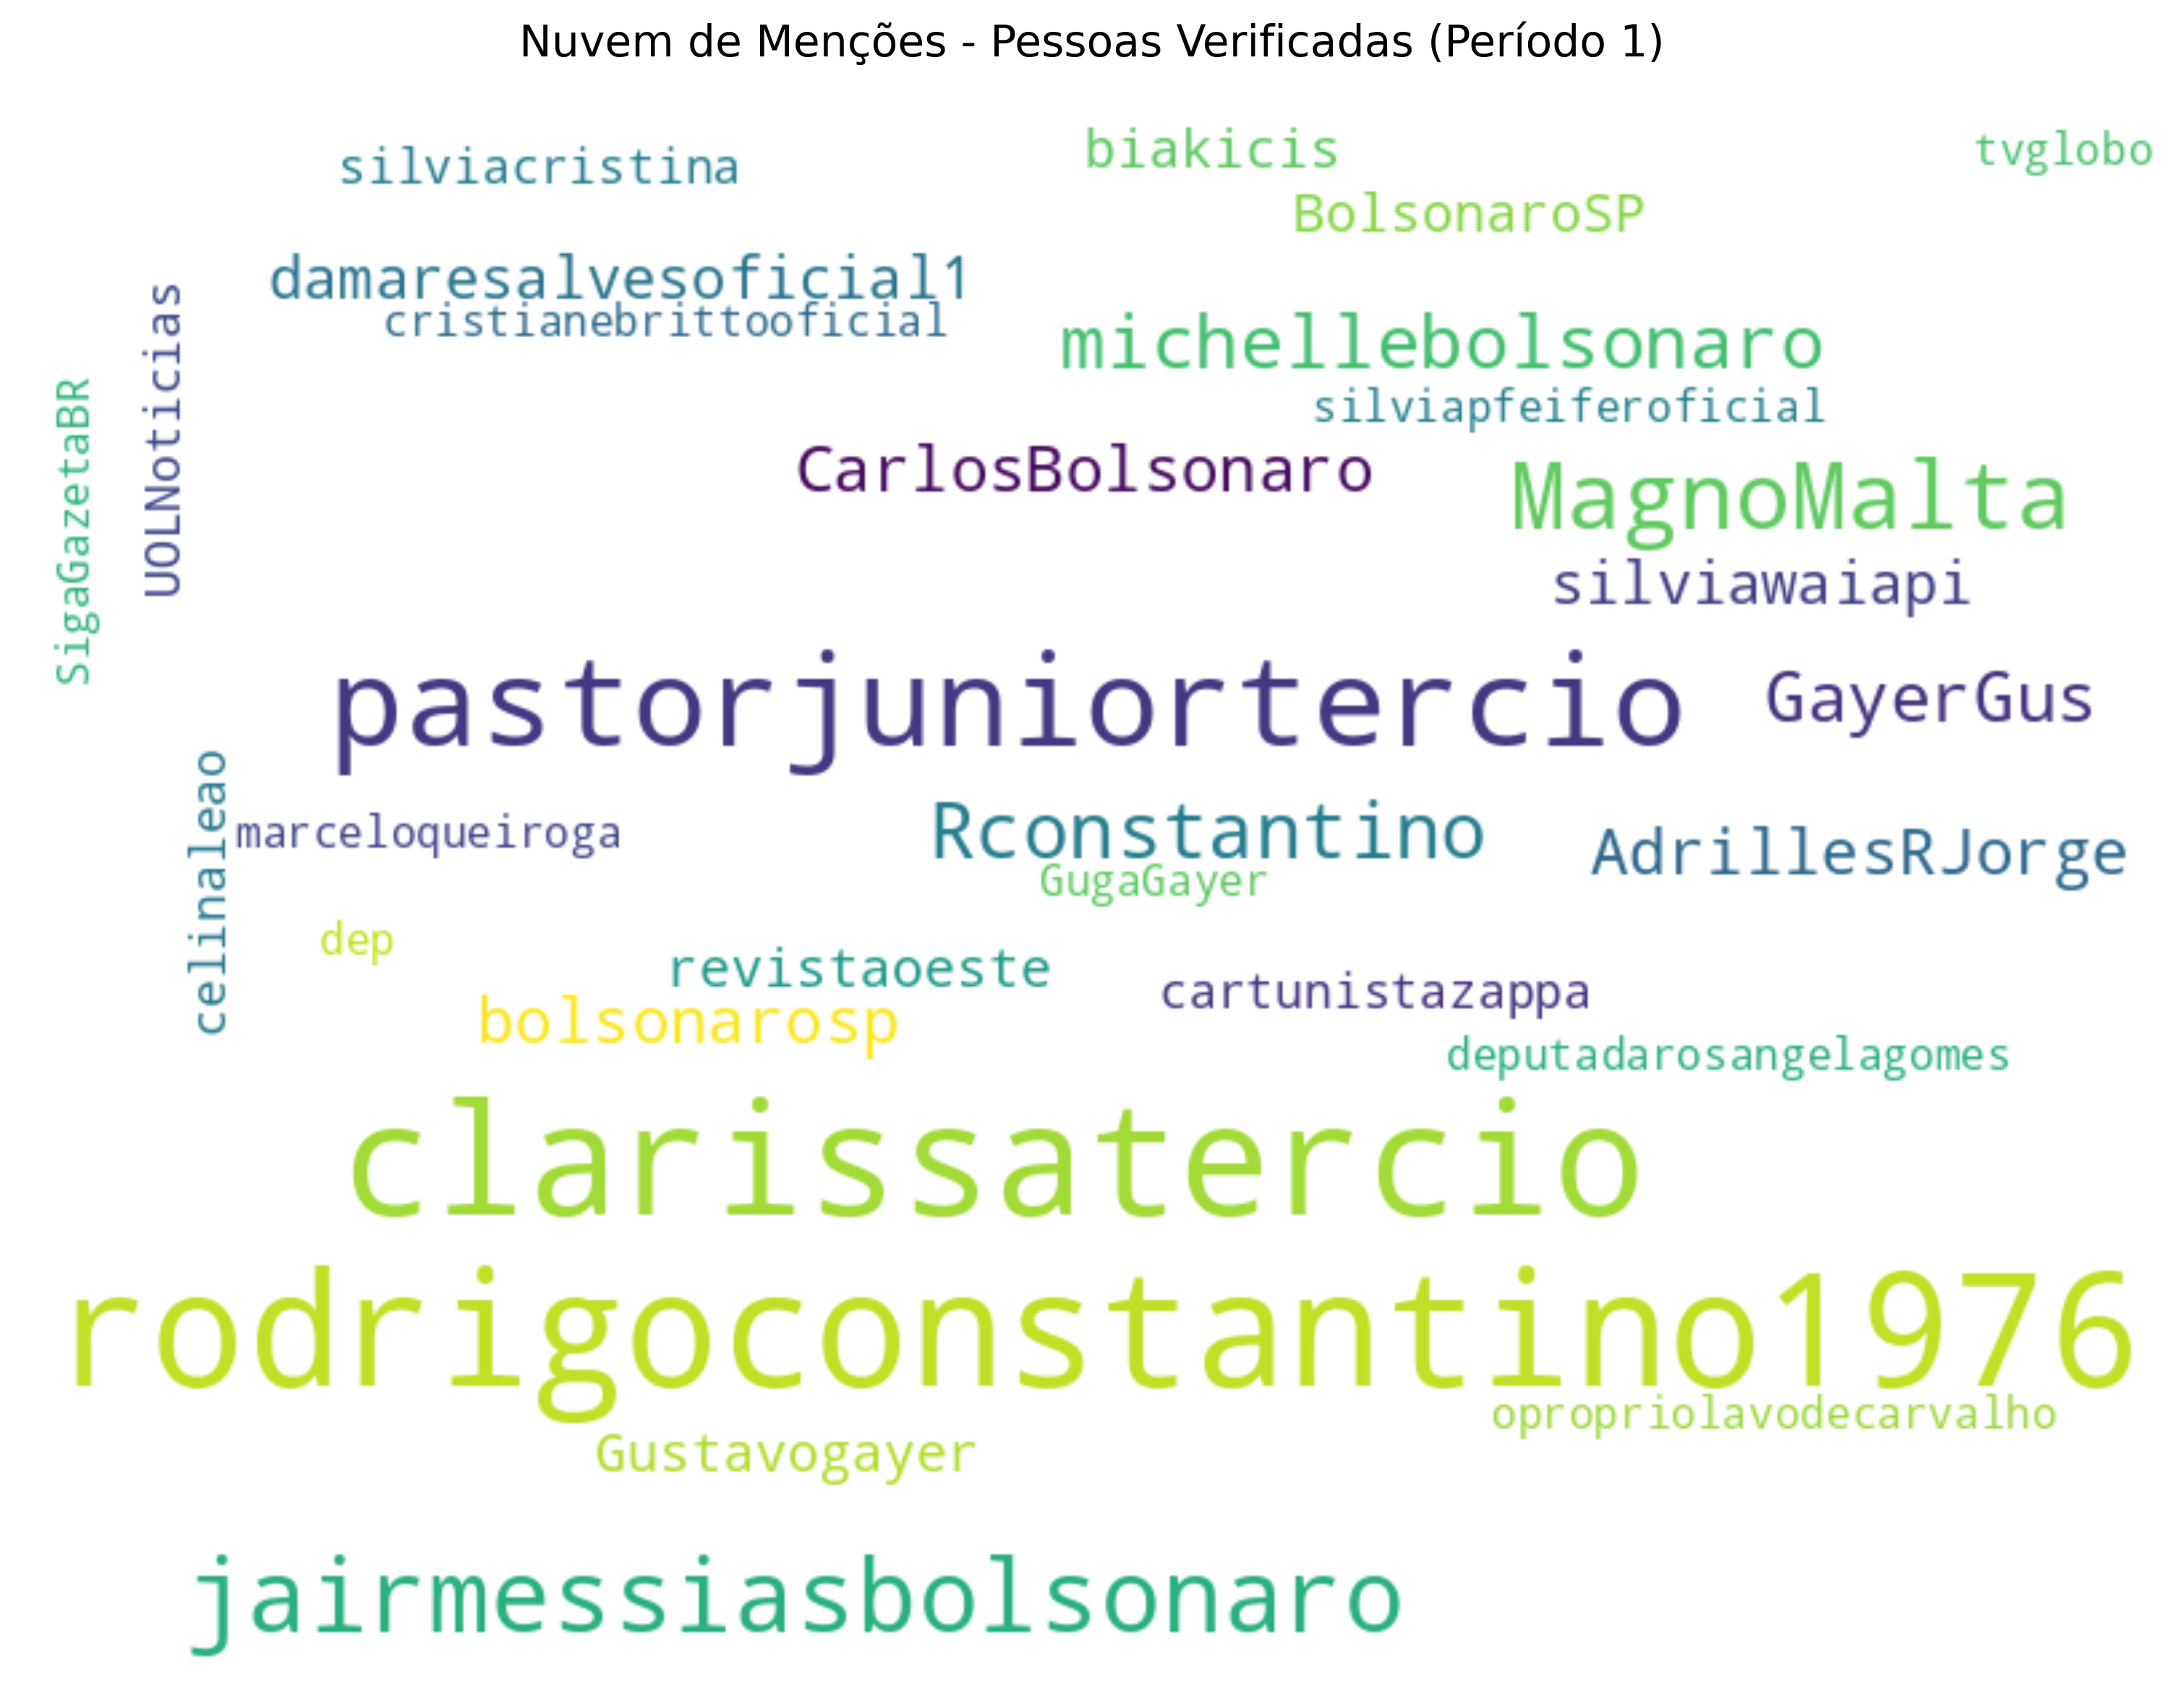
\includegraphics[width=0.8\textwidth]{figura13_mencoes_verificadas_periodo1.png}
\caption{Nuvem de menções - Pessoas verificadas (Período 1: 30/10/2022 a 08/01/2023).}
\label{fig:figura13}
\end{figure}

\begin{figure}[h]
\centering
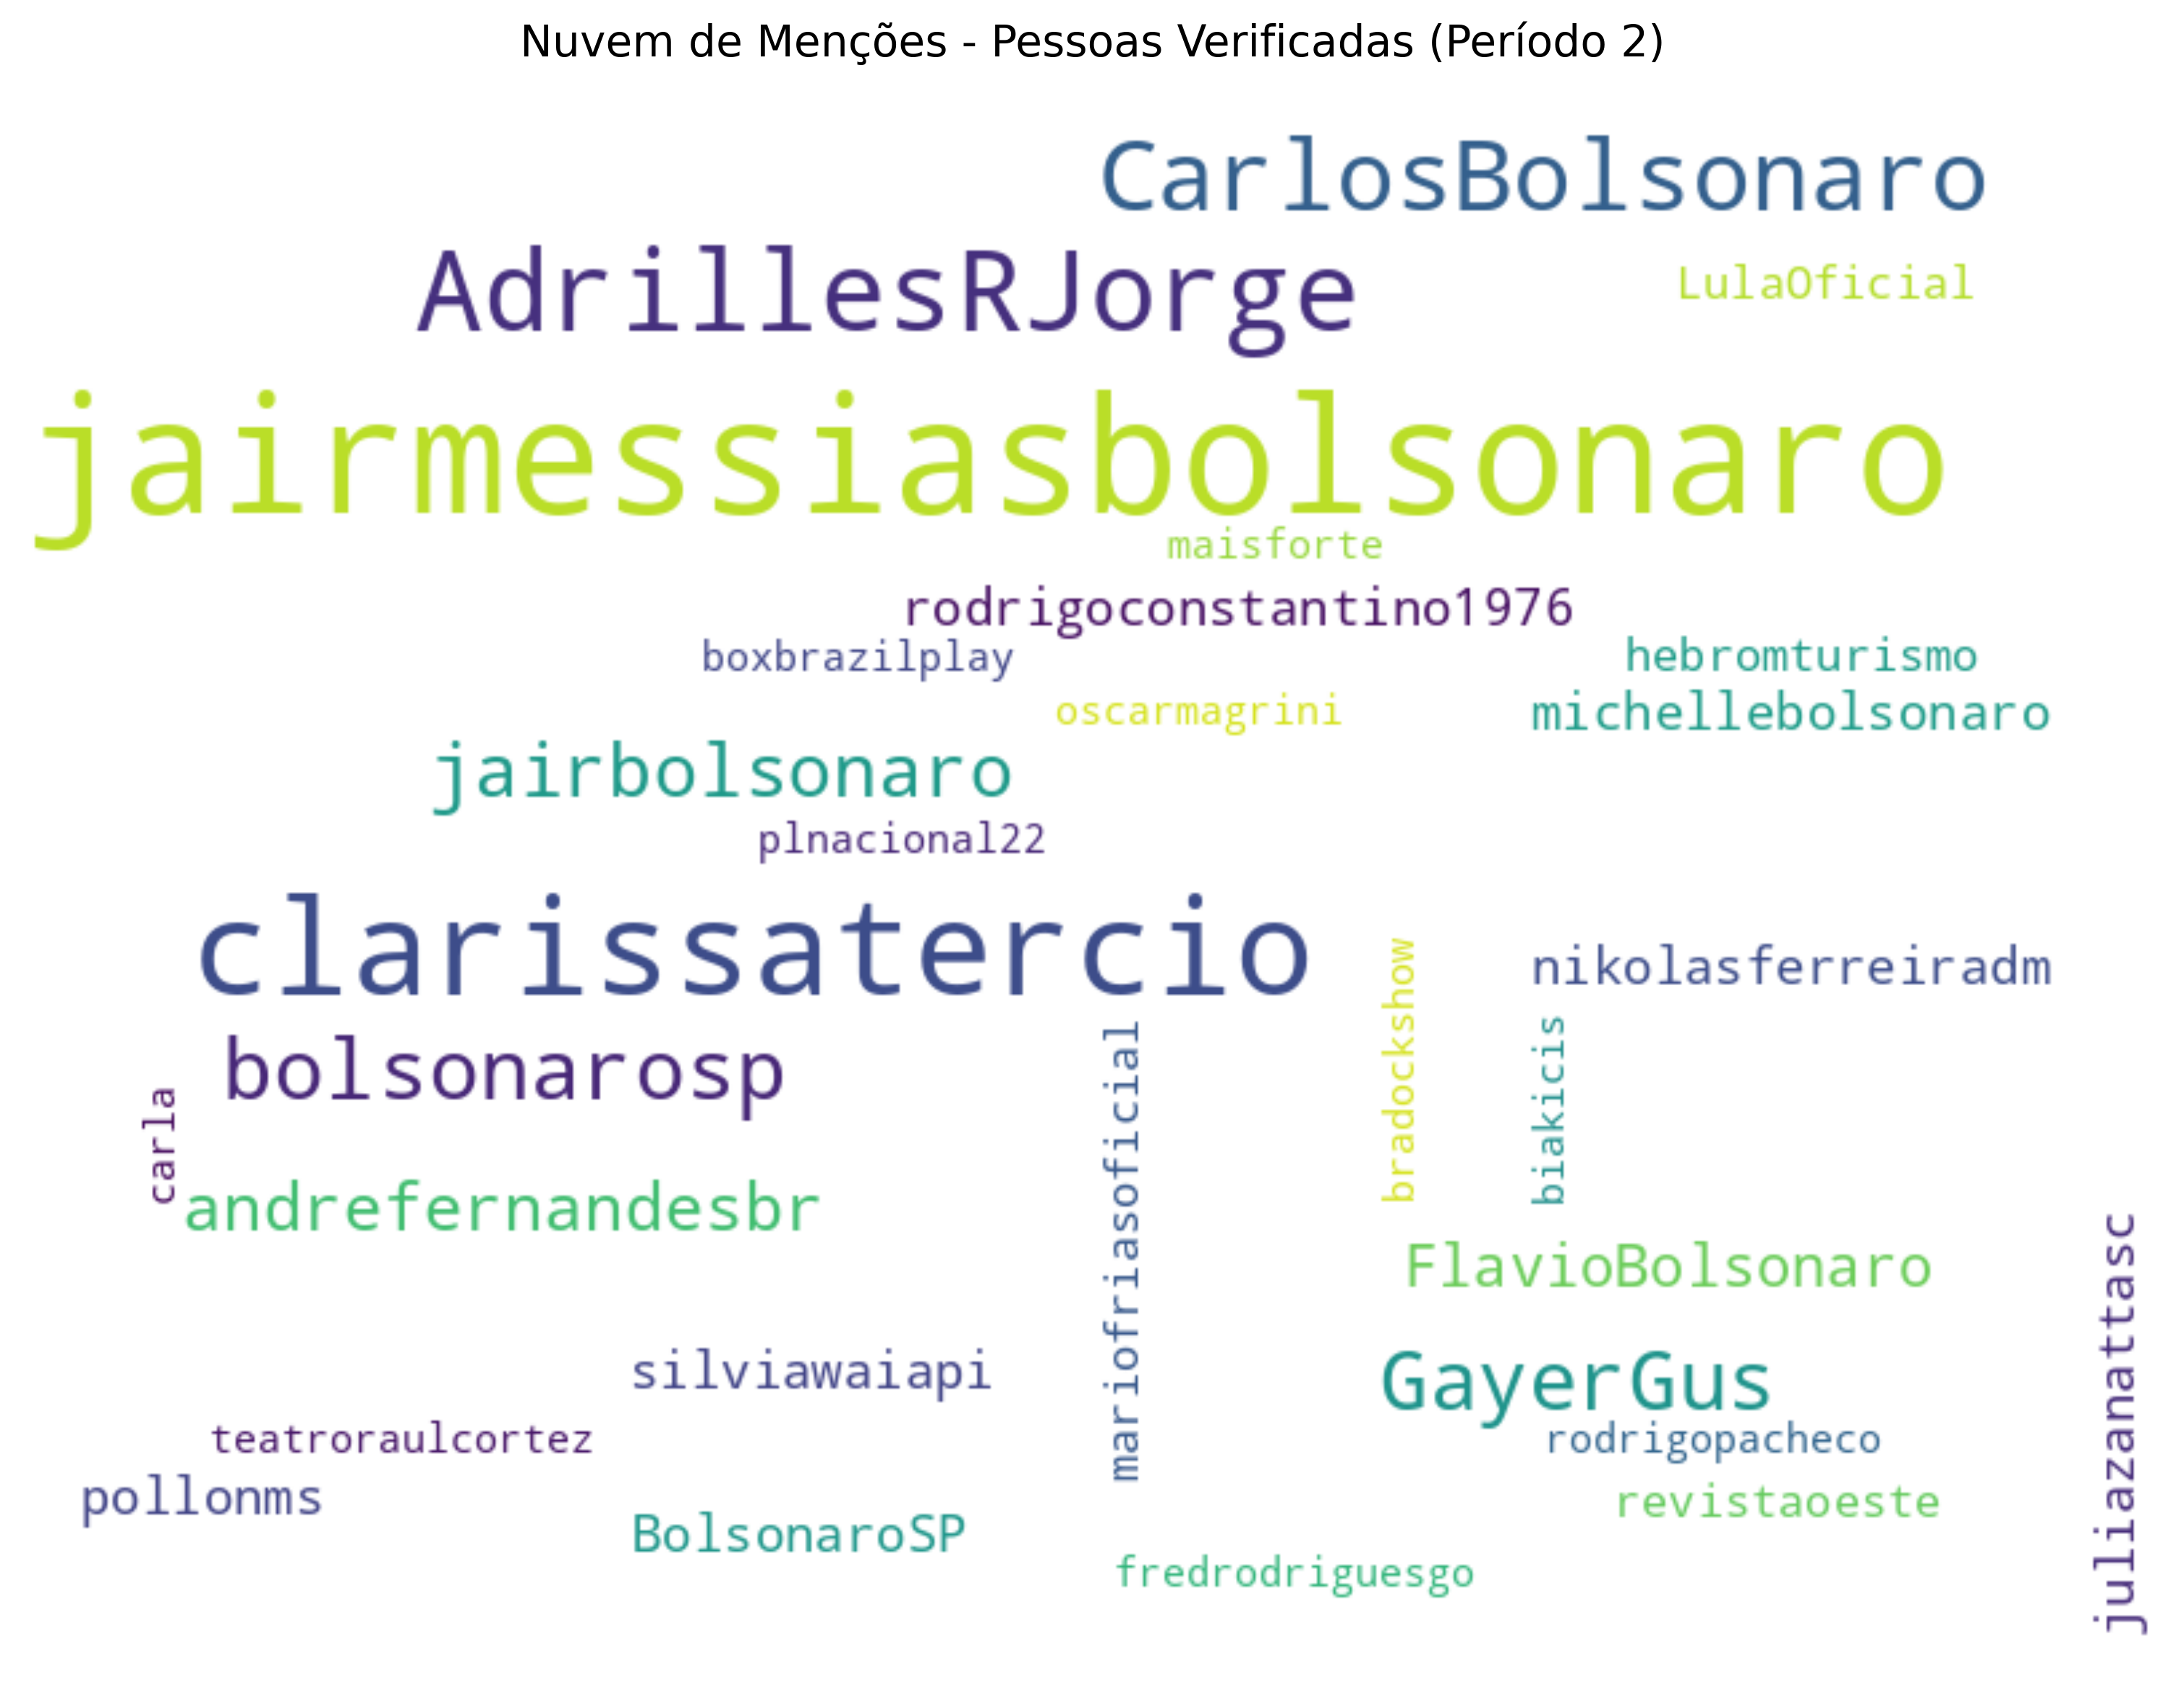
\includegraphics[width=0.8\textwidth]{figura14_mencoes_verificadas_periodo2.png}
\caption{Nuvem de menções - Pessoas verificadas (Período 2: 09/01/2023 a 10/04/2023).}
\label{fig:figura14}
\end{figure}

\begin{figure}[h]
\centering
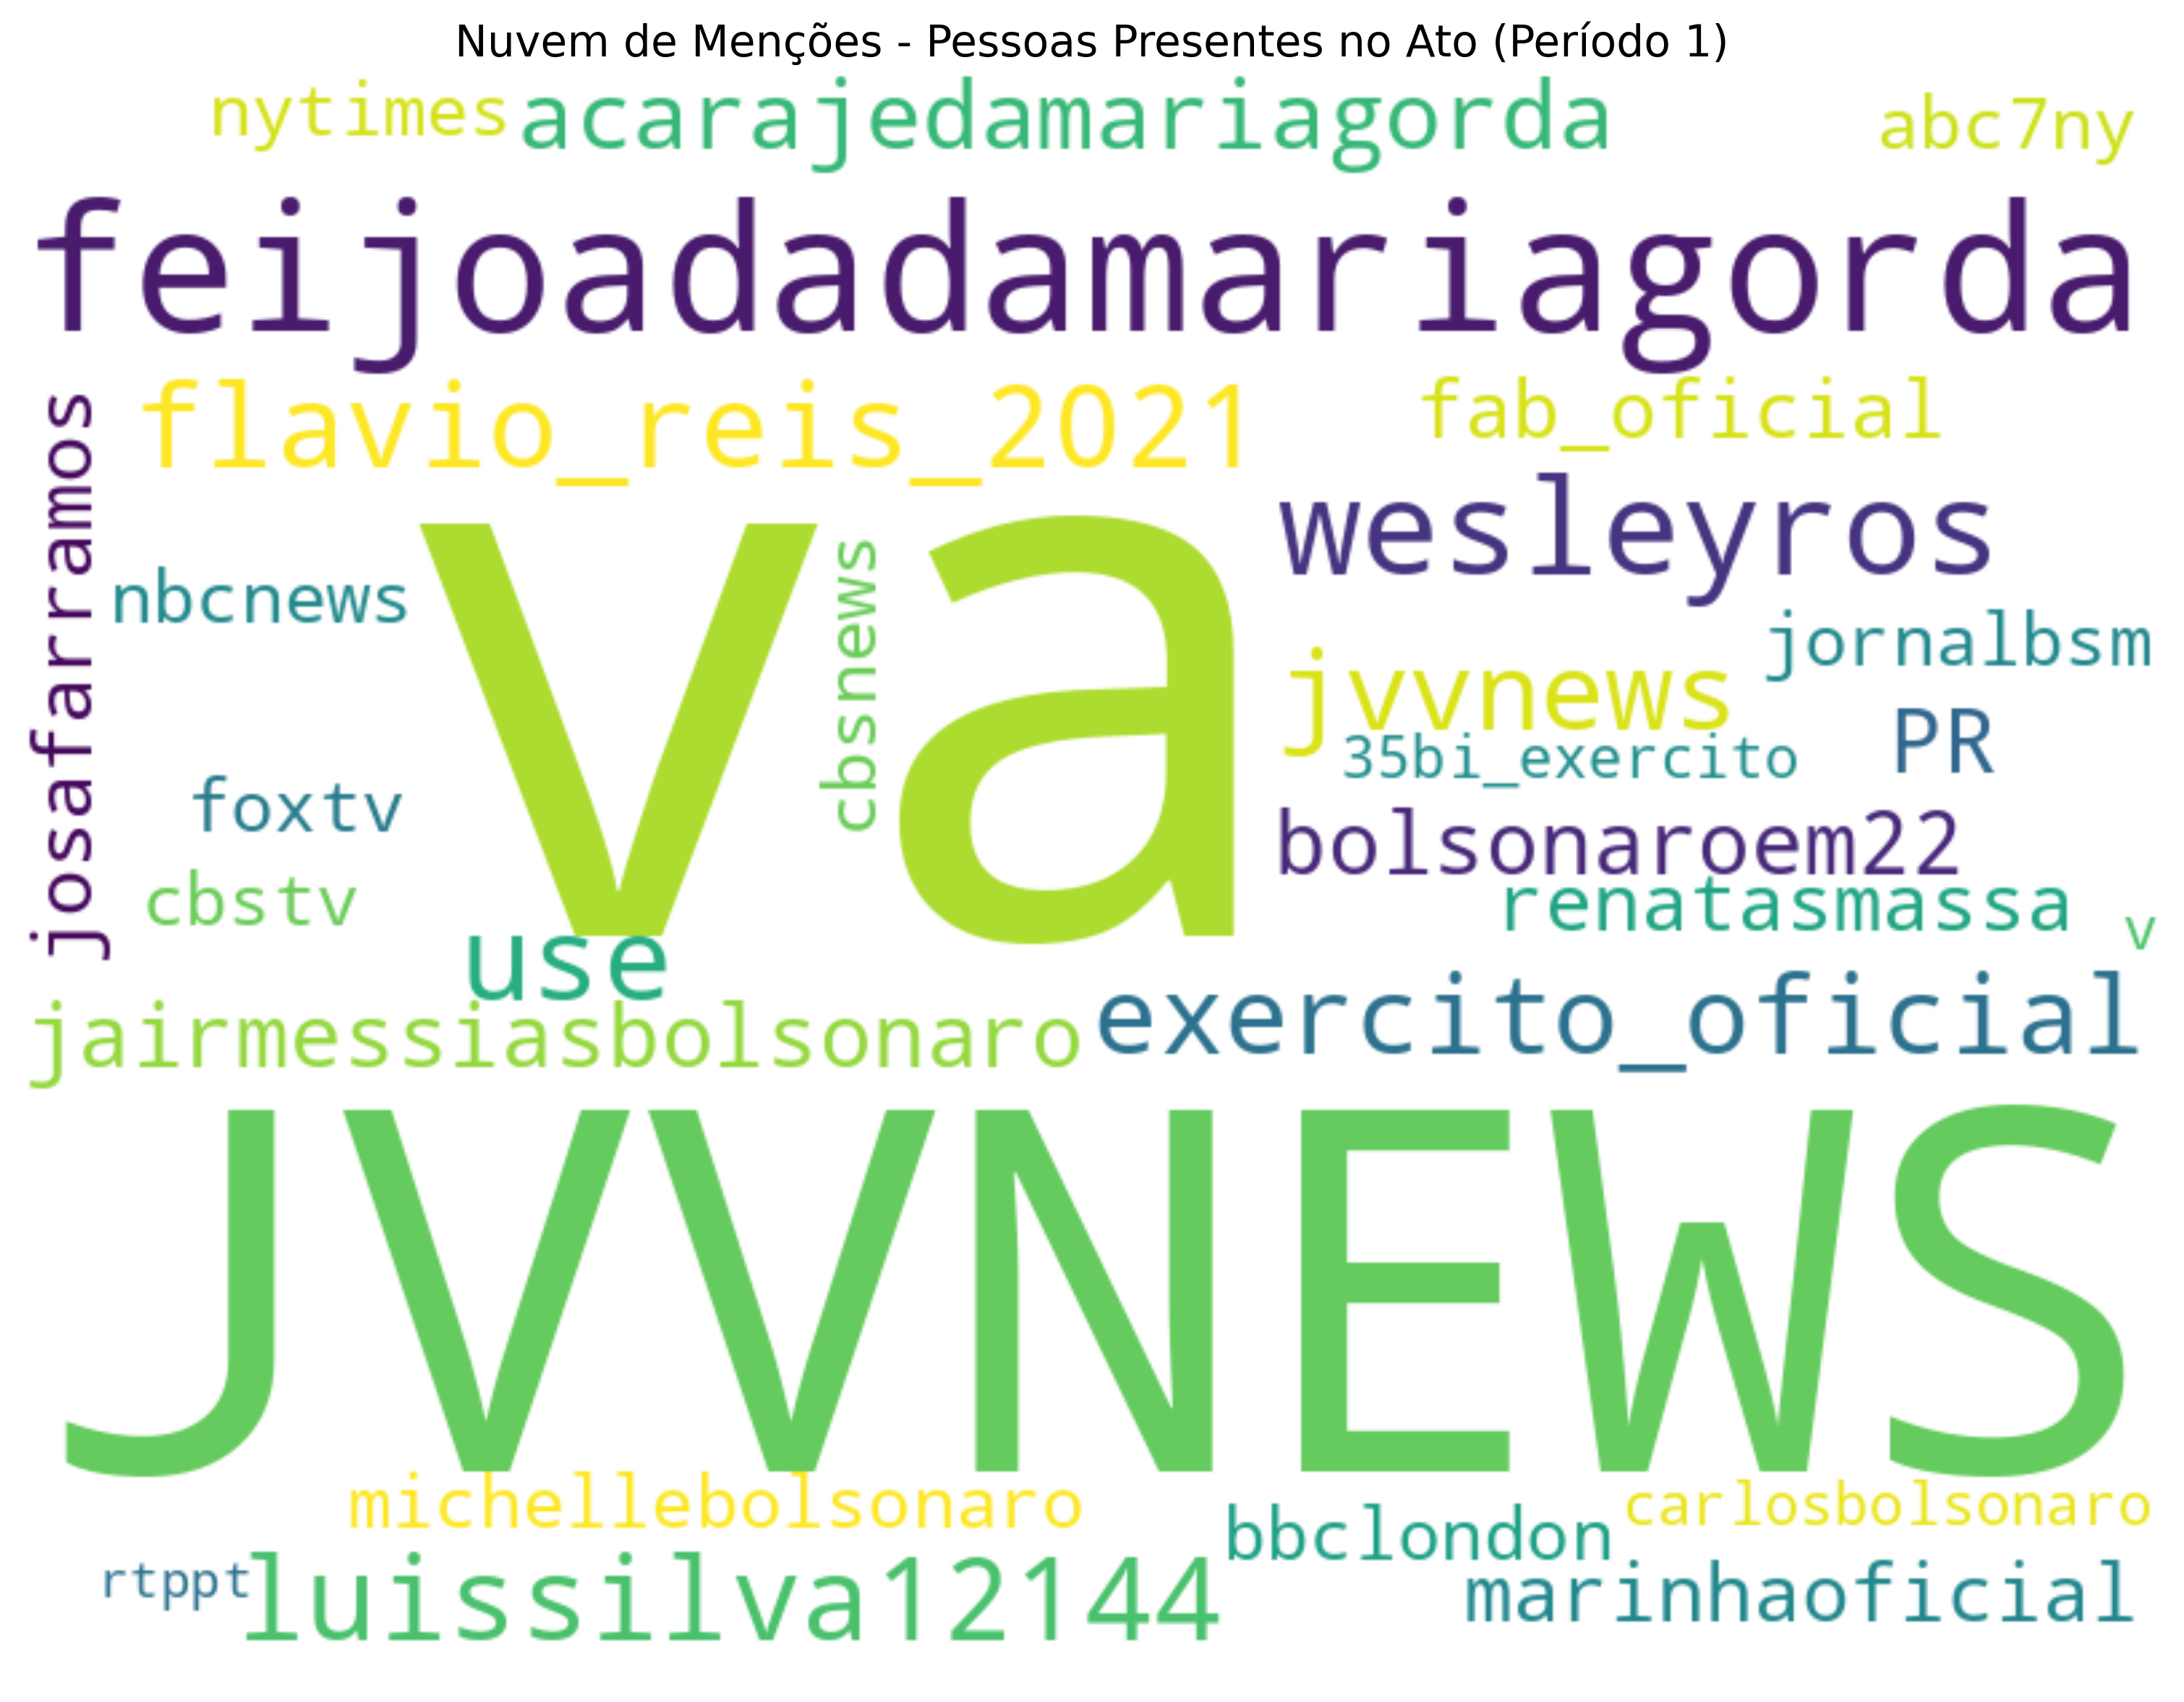
\includegraphics[width=0.8\textwidth]{figura15_mencoes_presentes_periodo1.png}
\caption{Nuvem de menções - Pessoas presentes no ato (Período 1: 30/10/2022 a 08/01/2023).}
\label{fig:figura15}
\end{figure}

\begin{figure}[h]
\centering
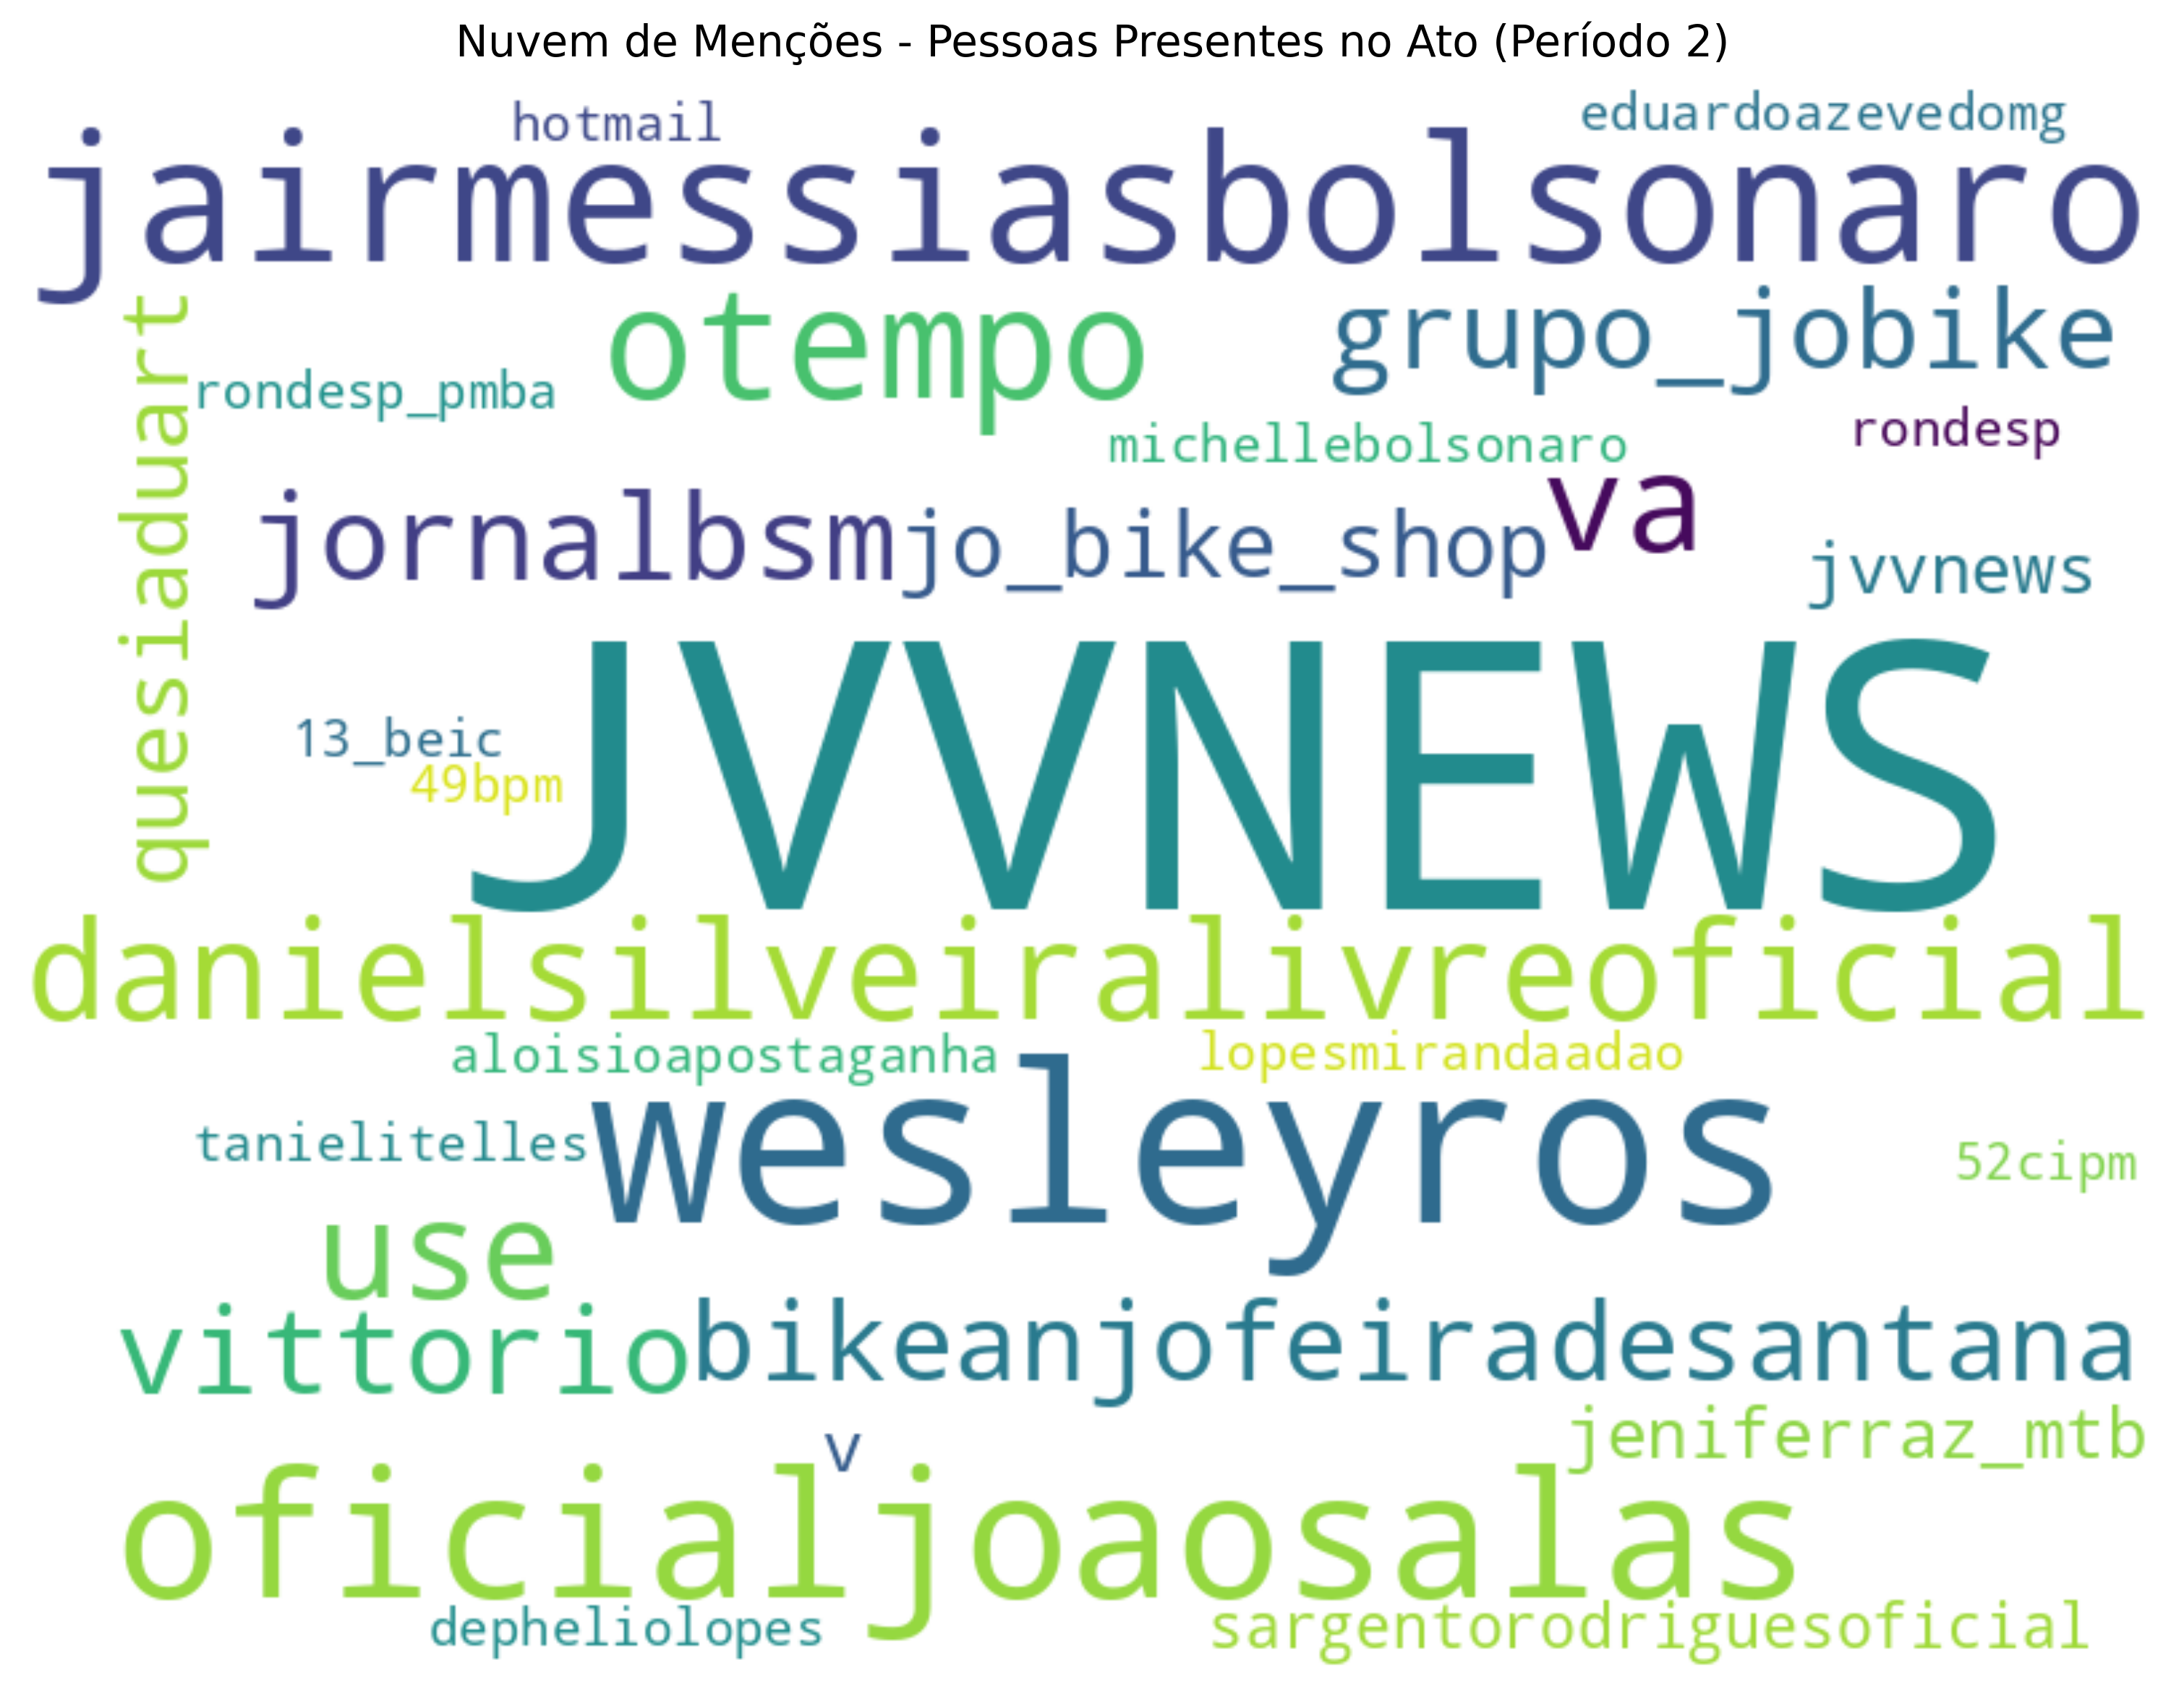
\includegraphics[width=0.8\textwidth]{figura16_mencoes_presentes_periodo2.png}
\caption{Nuvem de menções - Pessoas presentes no ato (Período 2: 09/01/2023 a 10/04/2023).}
\label{fig:figura16}
\end{figure}

\subsubsection{Nuvens de palavras}

\begin{figure}[h]
\centering
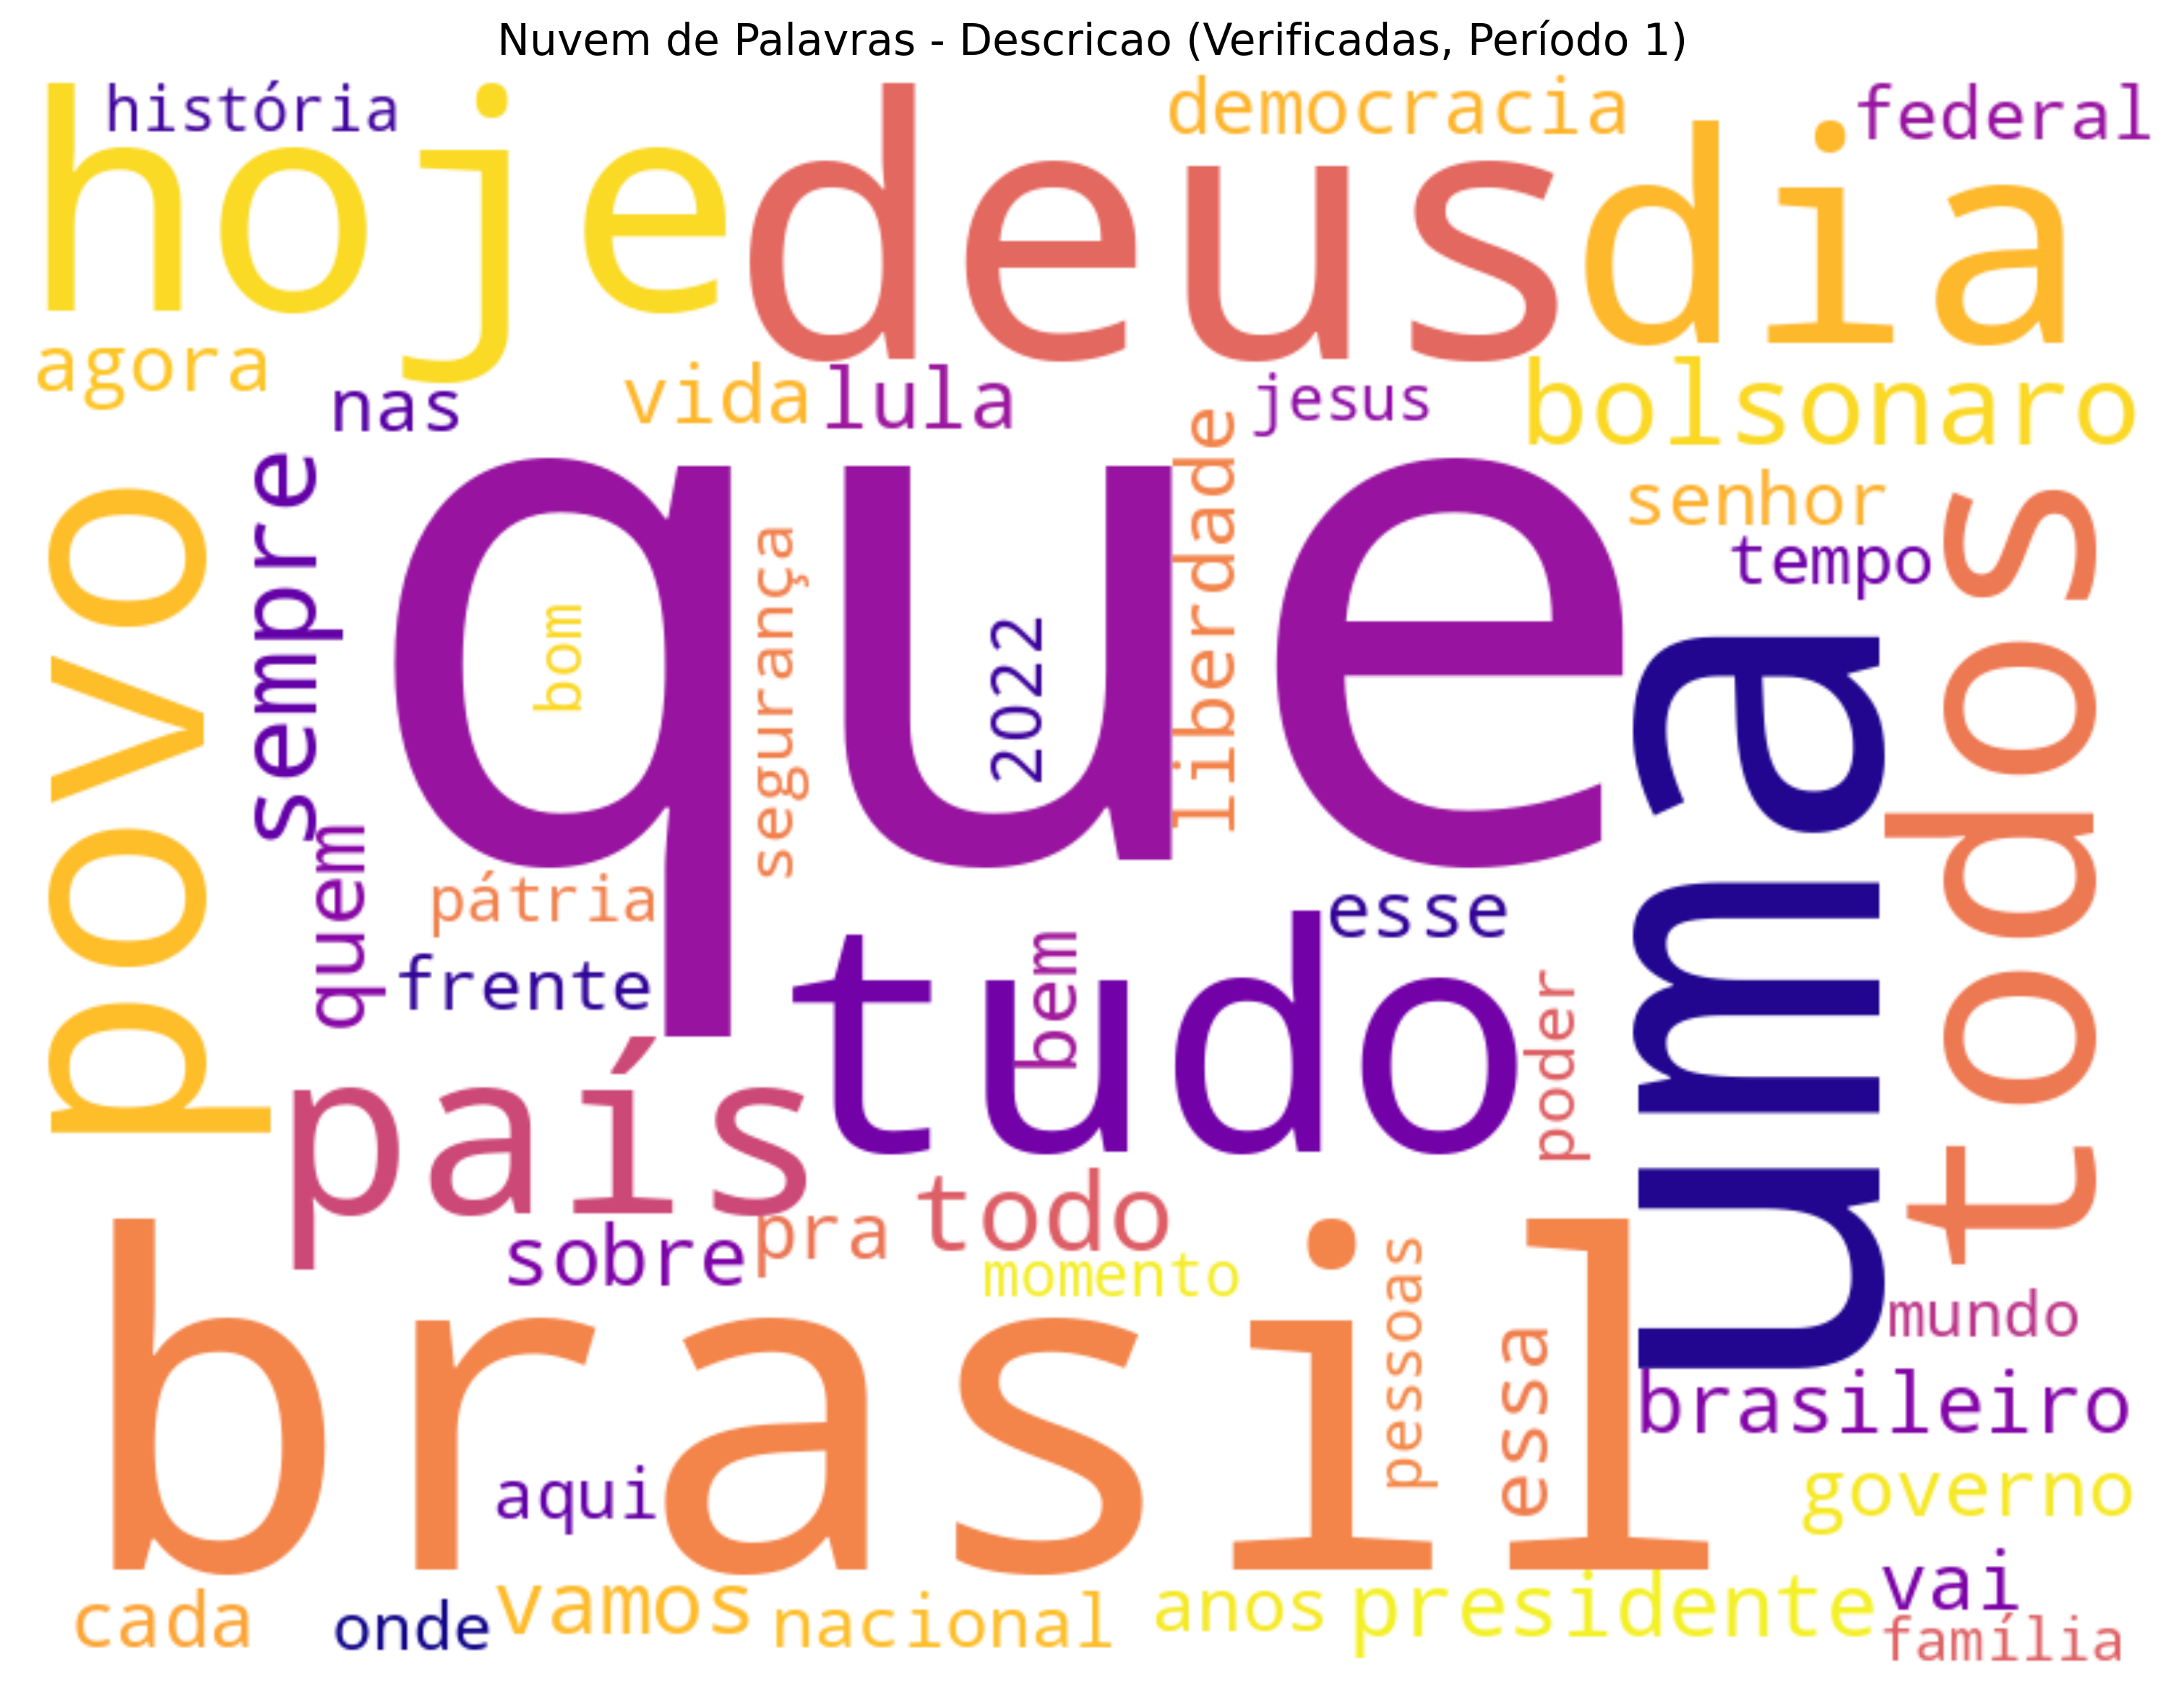
\includegraphics[width=0.8\textwidth]{figura17_nuvem_verificadas_desc_periodo1.png}
\caption{Nuvem de palavras - Descrições das pessoas verificadas (Período 1: 30/10/2022 a 08/01/2023).}
\label{fig:figura17}
\end{figure}

\begin{figure}[h]
\centering
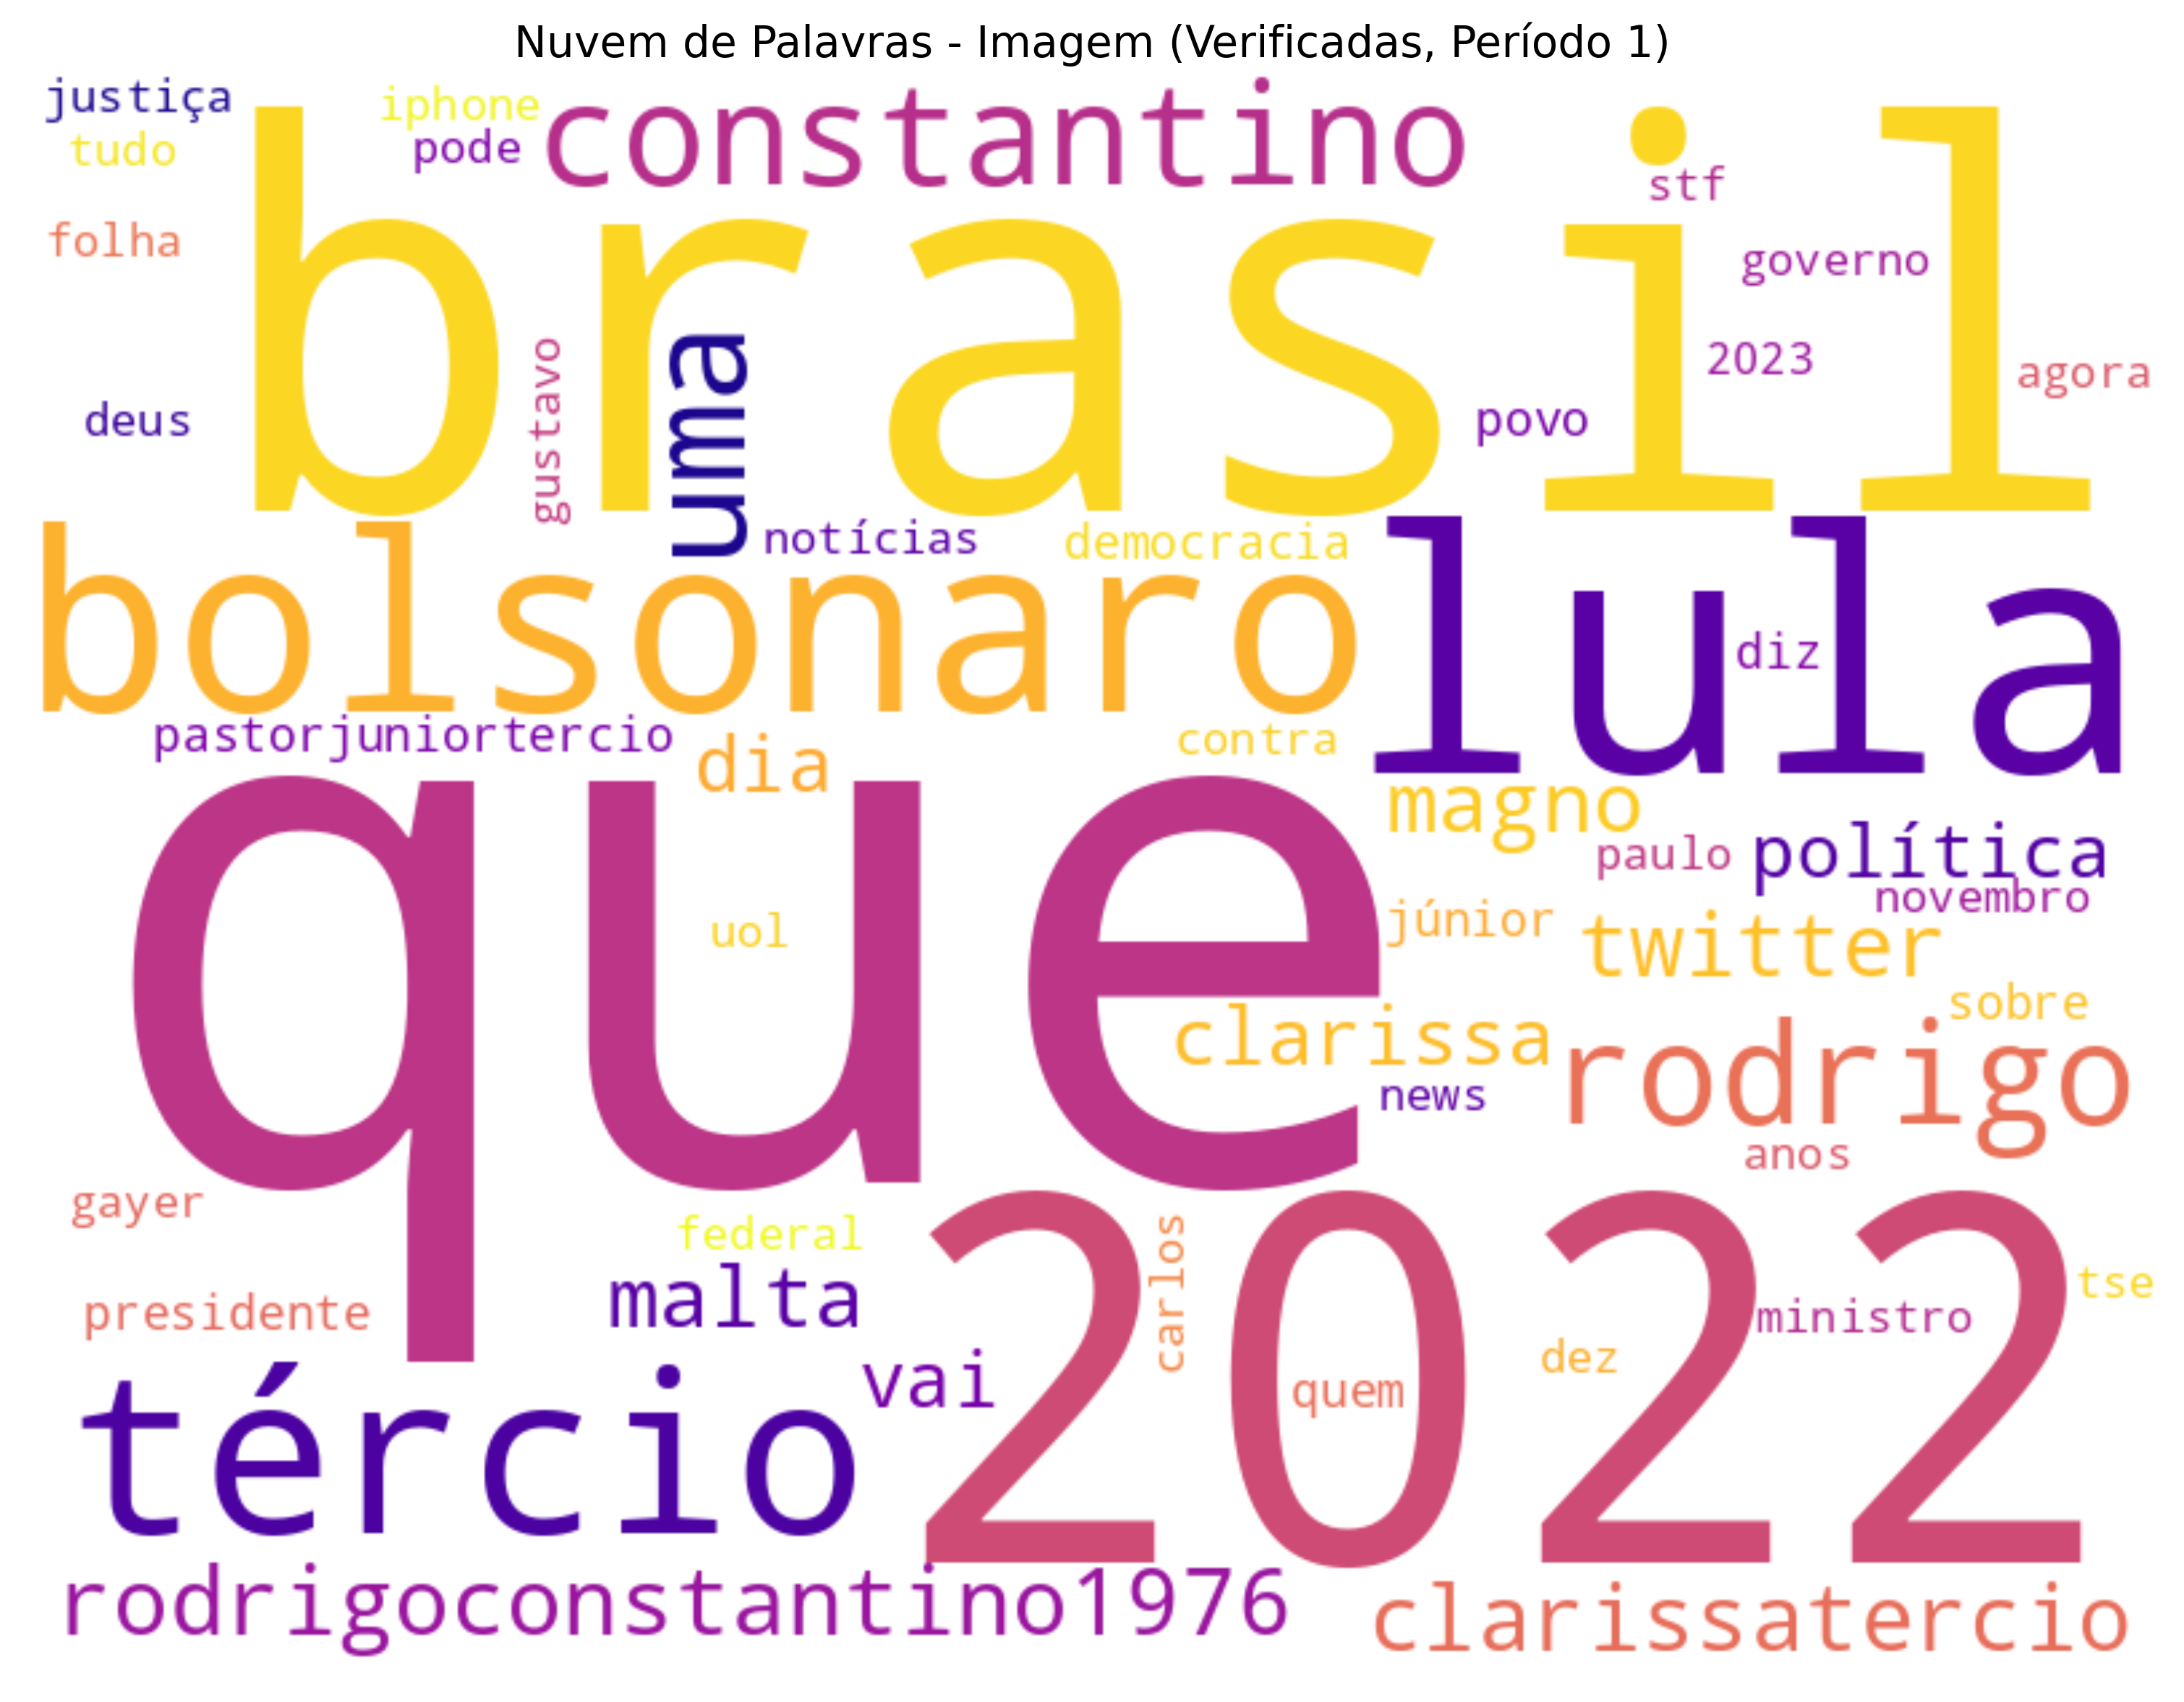
\includegraphics[width=0.8\textwidth]{figura18_nuvem_verificadas_img_periodo1.png}
\caption{Nuvem de palavras - Texto das imagens das pessoas verificadas (Período 1: 30/10/2022 a 08/01/2023).}
\label{fig:figura18}
\end{figure}

\begin{figure}[h]
\centering
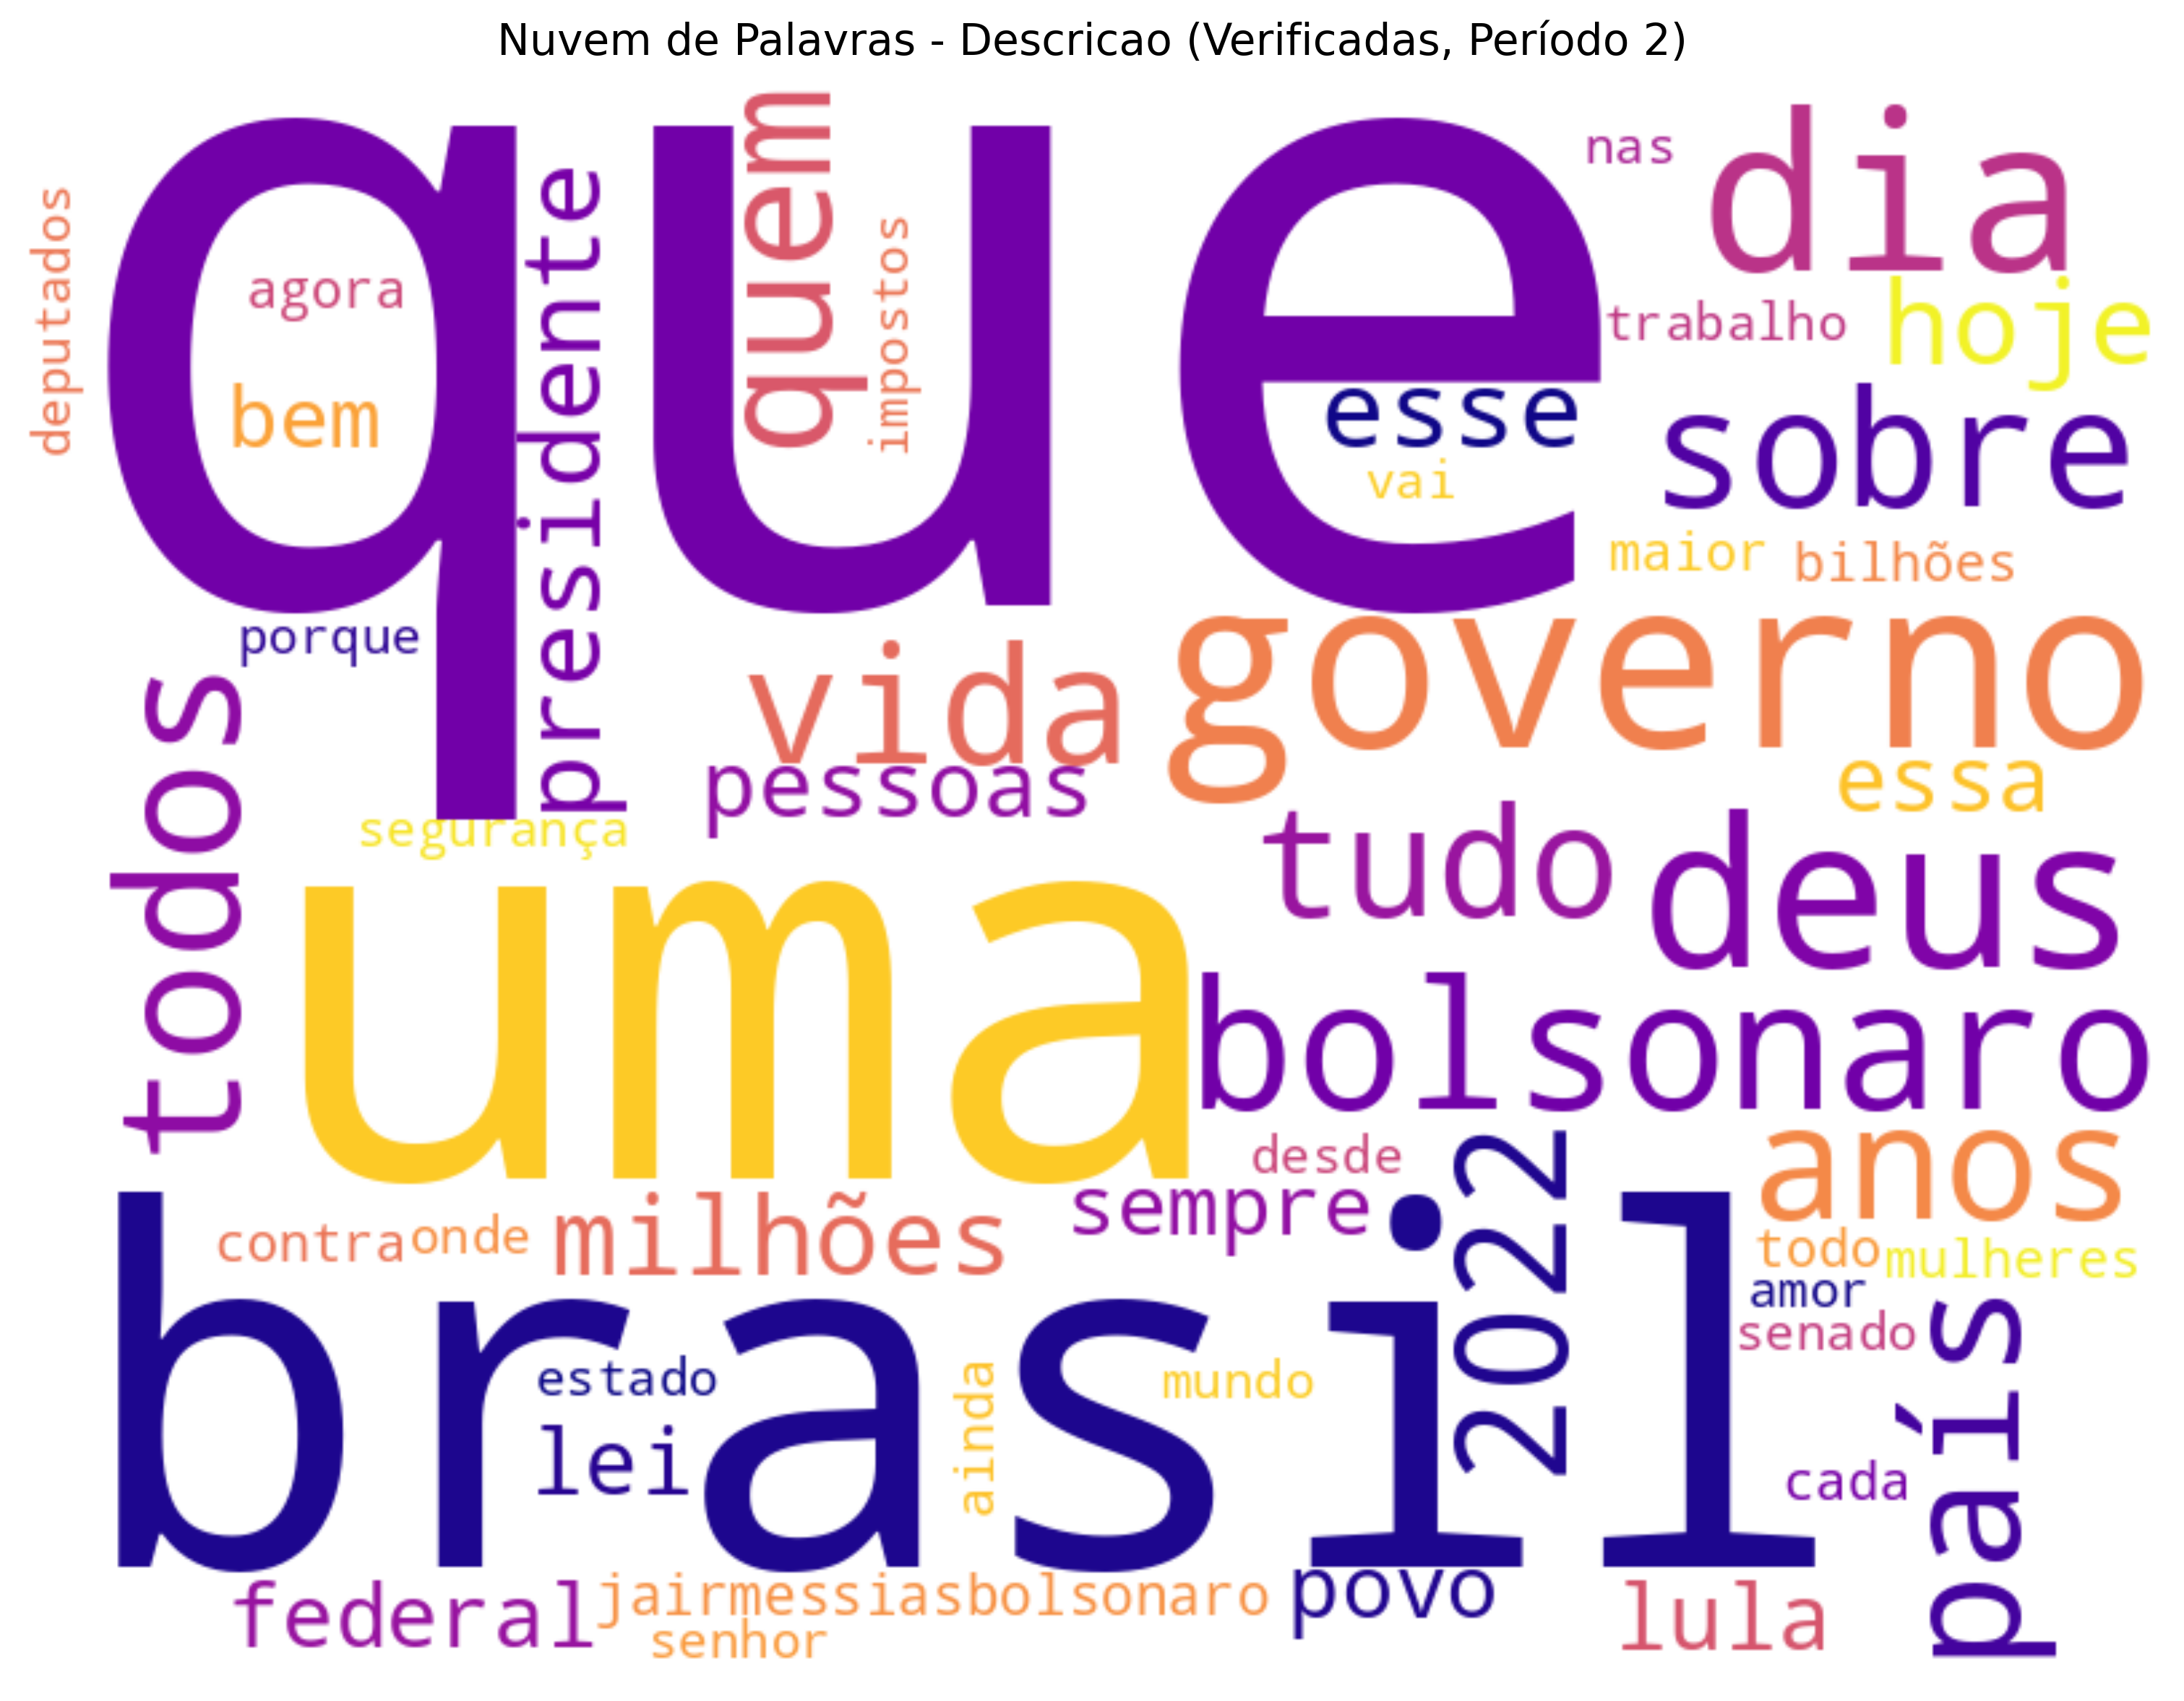
\includegraphics[width=0.8\textwidth]{figura19_nuvem_verificadas_desc_periodo2.png}
\caption{Nuvem de palavras - Descrições das pessoas verificadas (Período 2: 09/01/2023 a 10/04/2023).}
\label{fig:figura19}
\end{figure}

\begin{figure}[h]
\centering
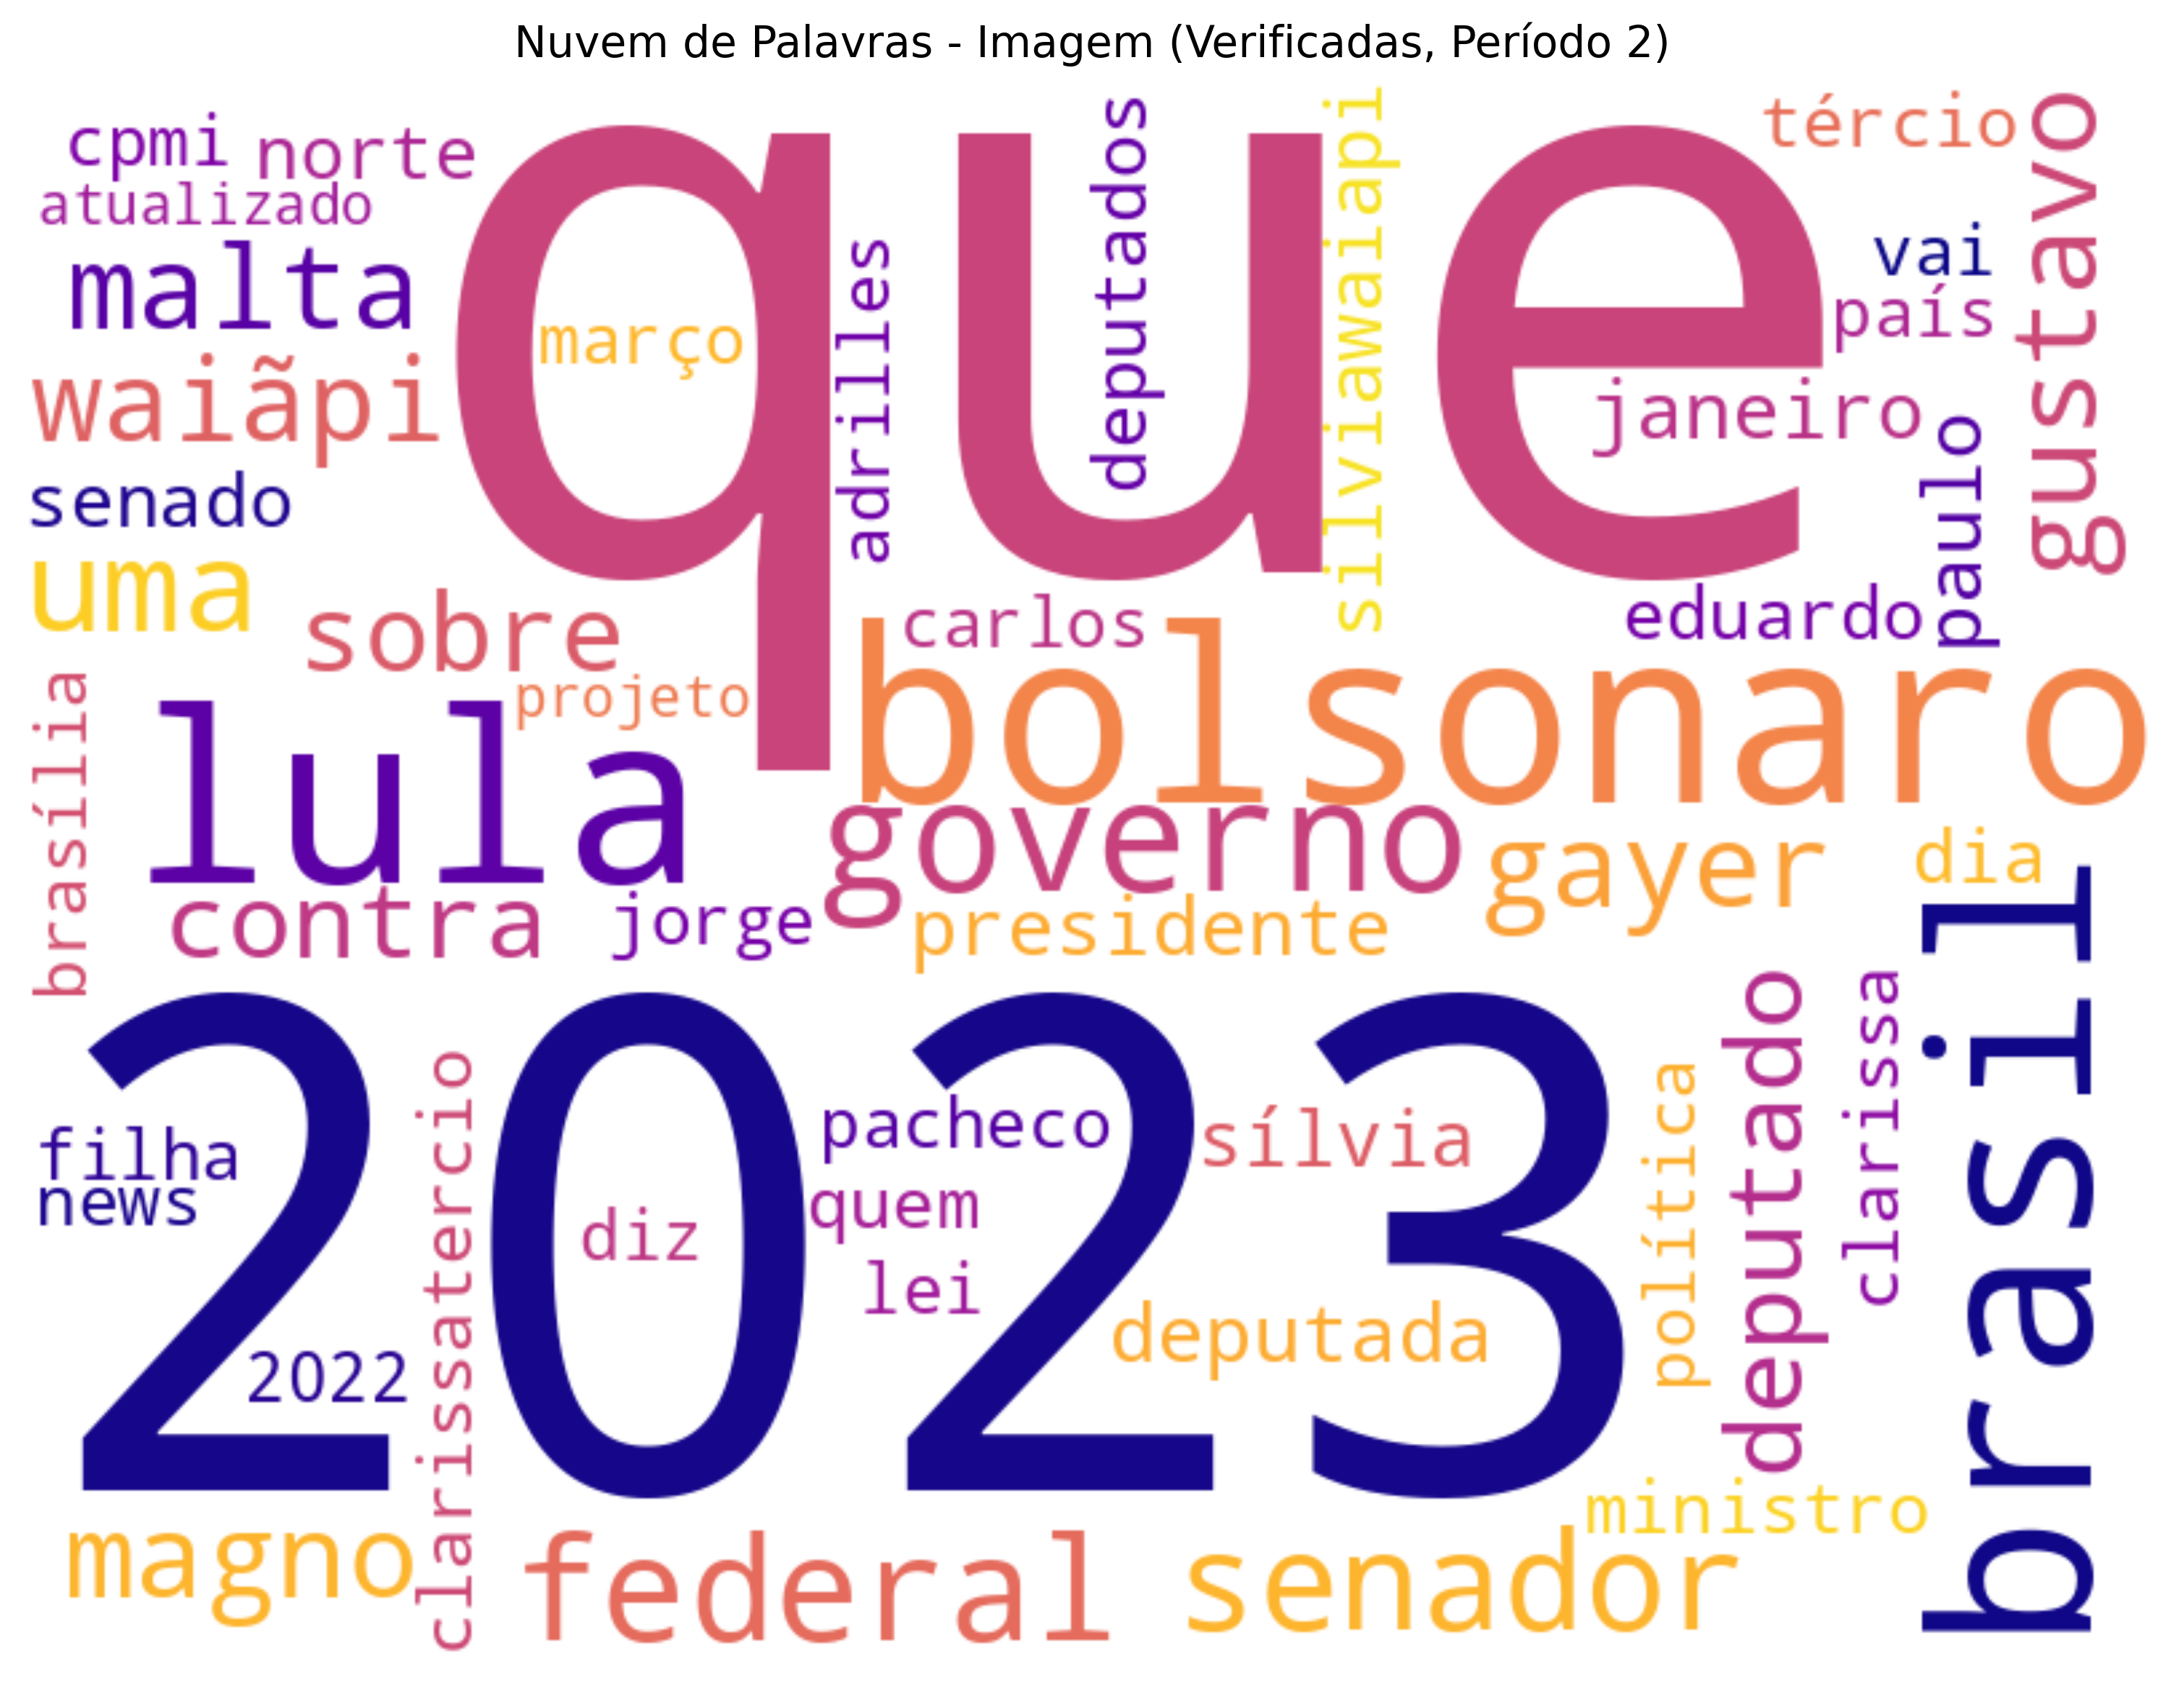
\includegraphics[width=0.8\textwidth]{figura20_nuvem_verificadas_img_periodo2.png}
\caption{Nuvem de palavras - Texto das imagens das pessoas verificadas (Período 2: 09/01/2023 a 10/04/2023).}
\label{fig:figura20}
\end{figure}

\begin{figure}[h]
\centering
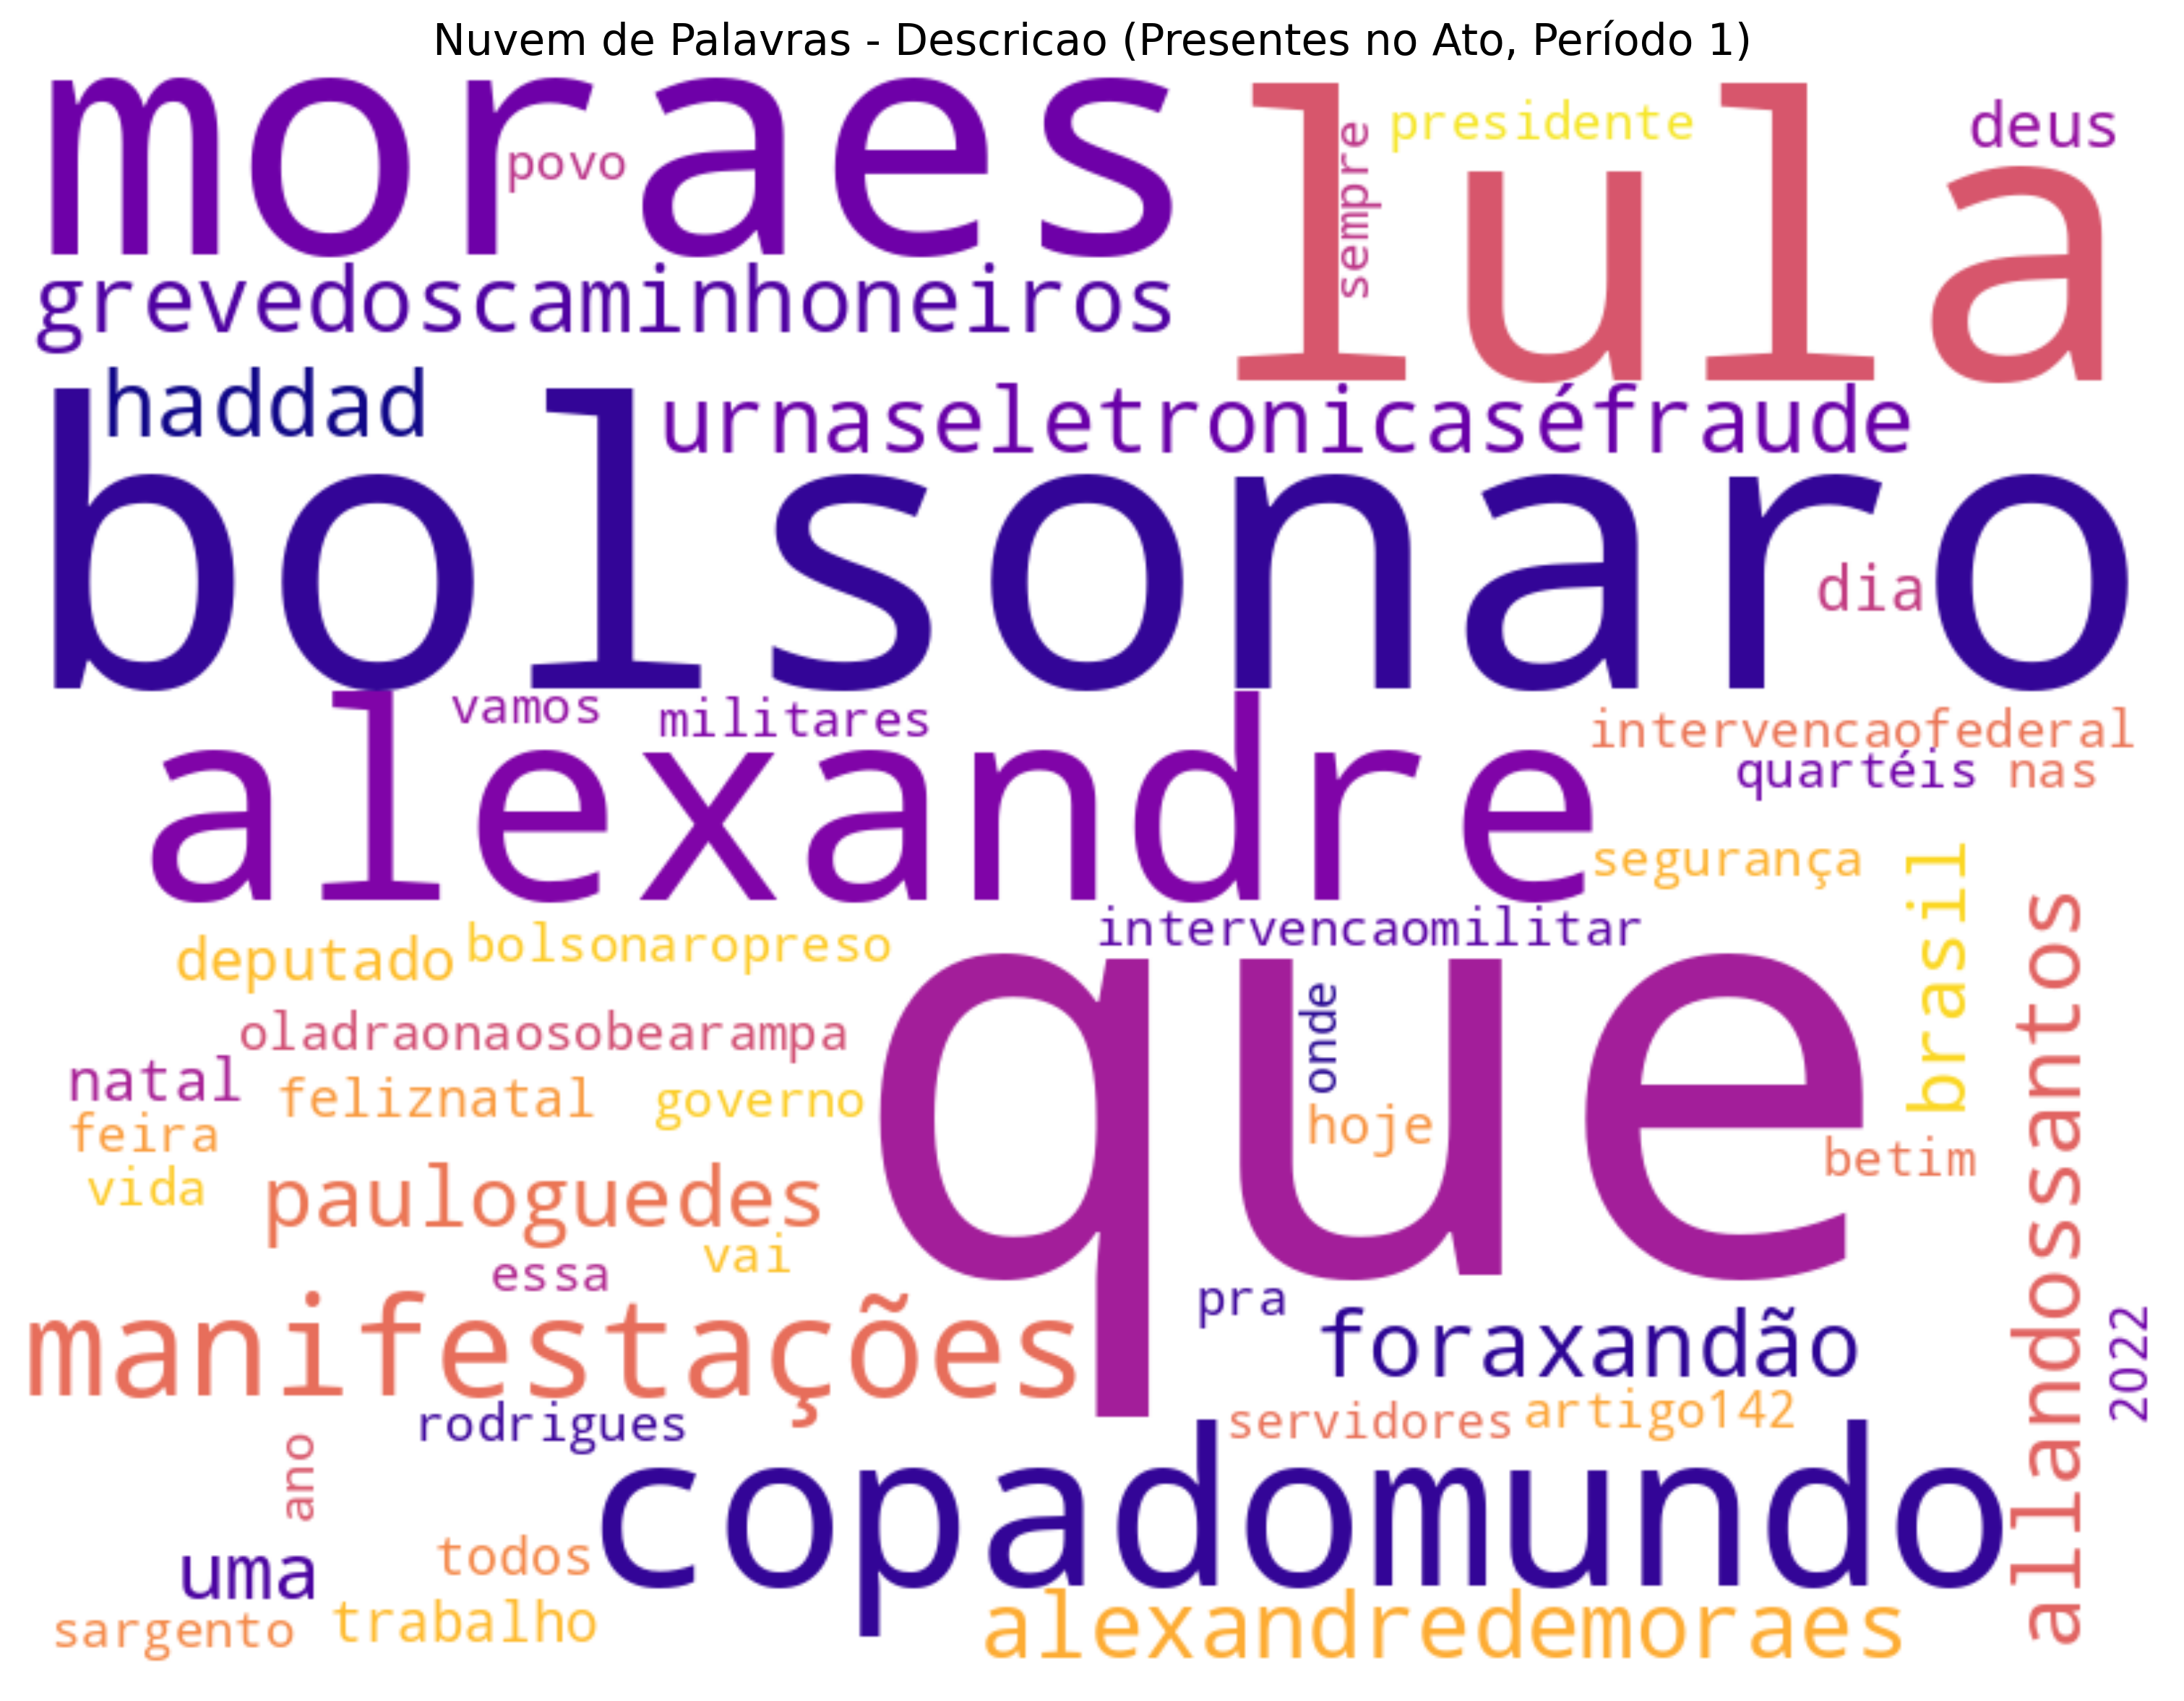
\includegraphics[width=0.8\textwidth]{figura21_nuvem_presentes_desc_periodo1.png}
\caption{Nuvem de palavras - Descrições das pessoas presentes no ato (Período 1: 30/10/2022 a 08/01/2023).}
\label{fig:figura21}
\end{figure}

\begin{figure}[h]
\centering
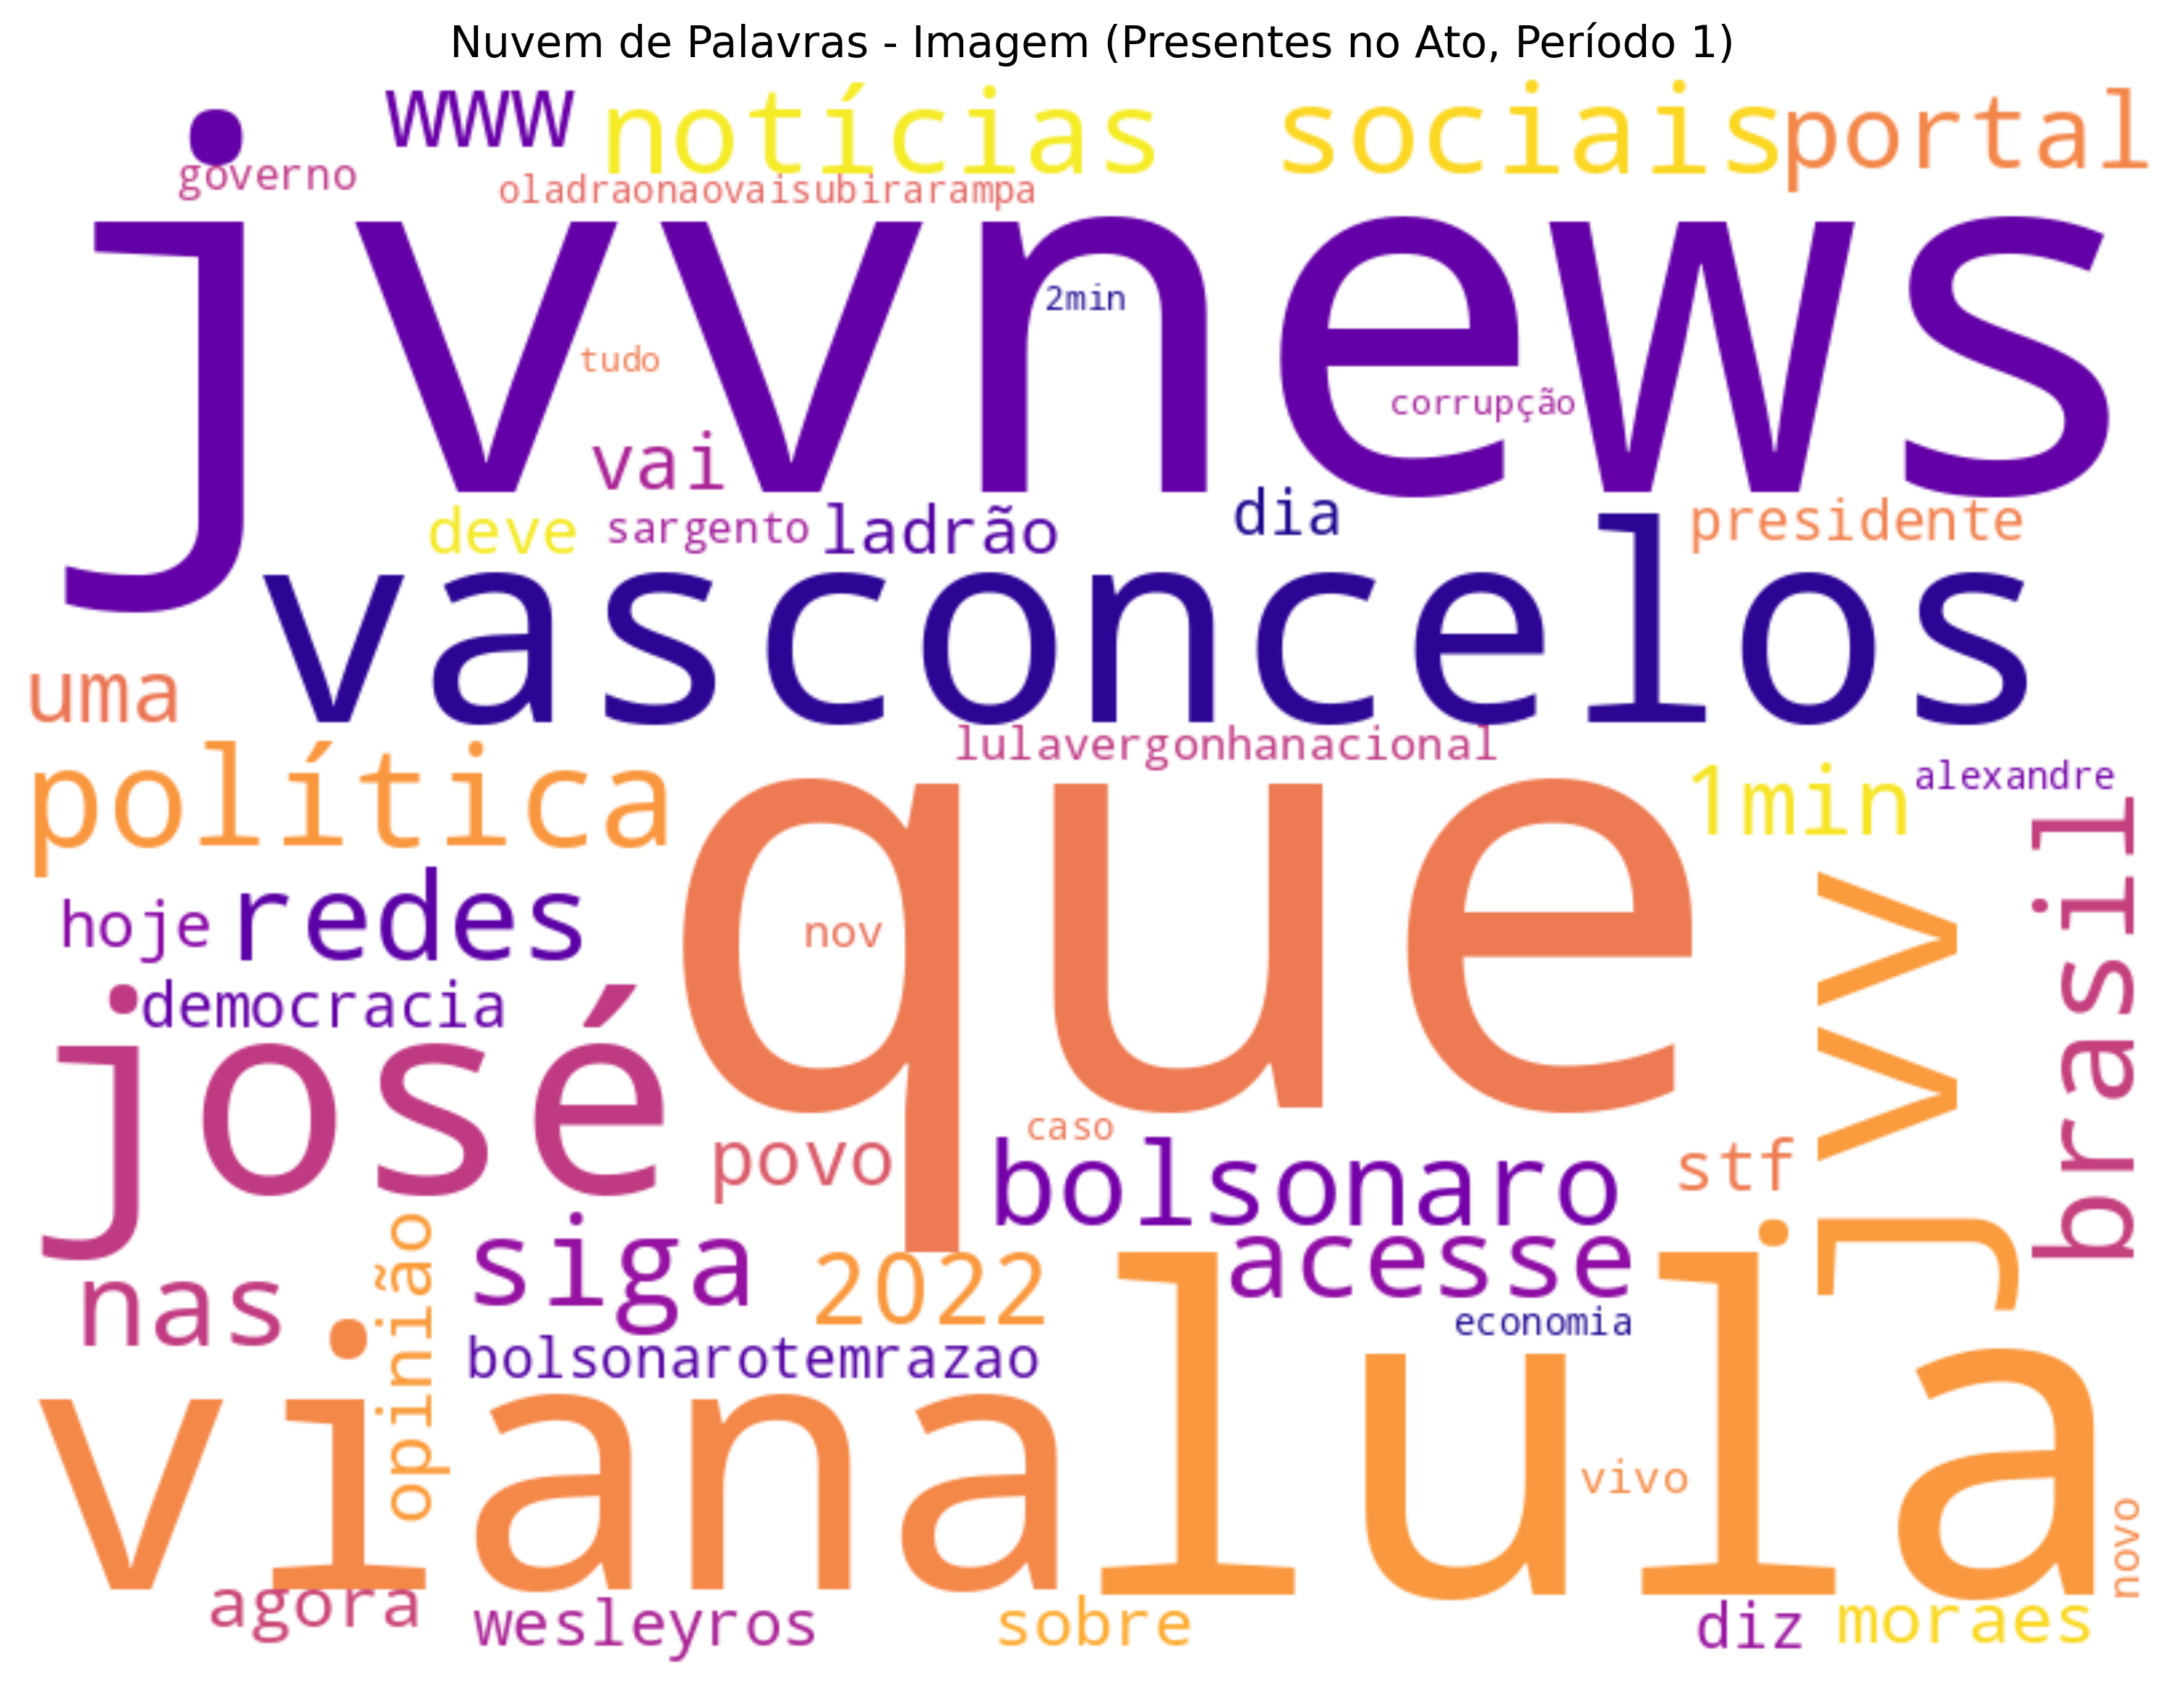
\includegraphics[width=0.8\textwidth]{figura22_nuvem_presentes_img_periodo1.png}
\caption{Nuvem de palavras - Texto das imagens das pessoas presentes no ato (Período 1: 30/10/2022 a 08/01/2023).}
\label{fig:figura22}
\end{figure}

\begin{figure}[h]
\centering
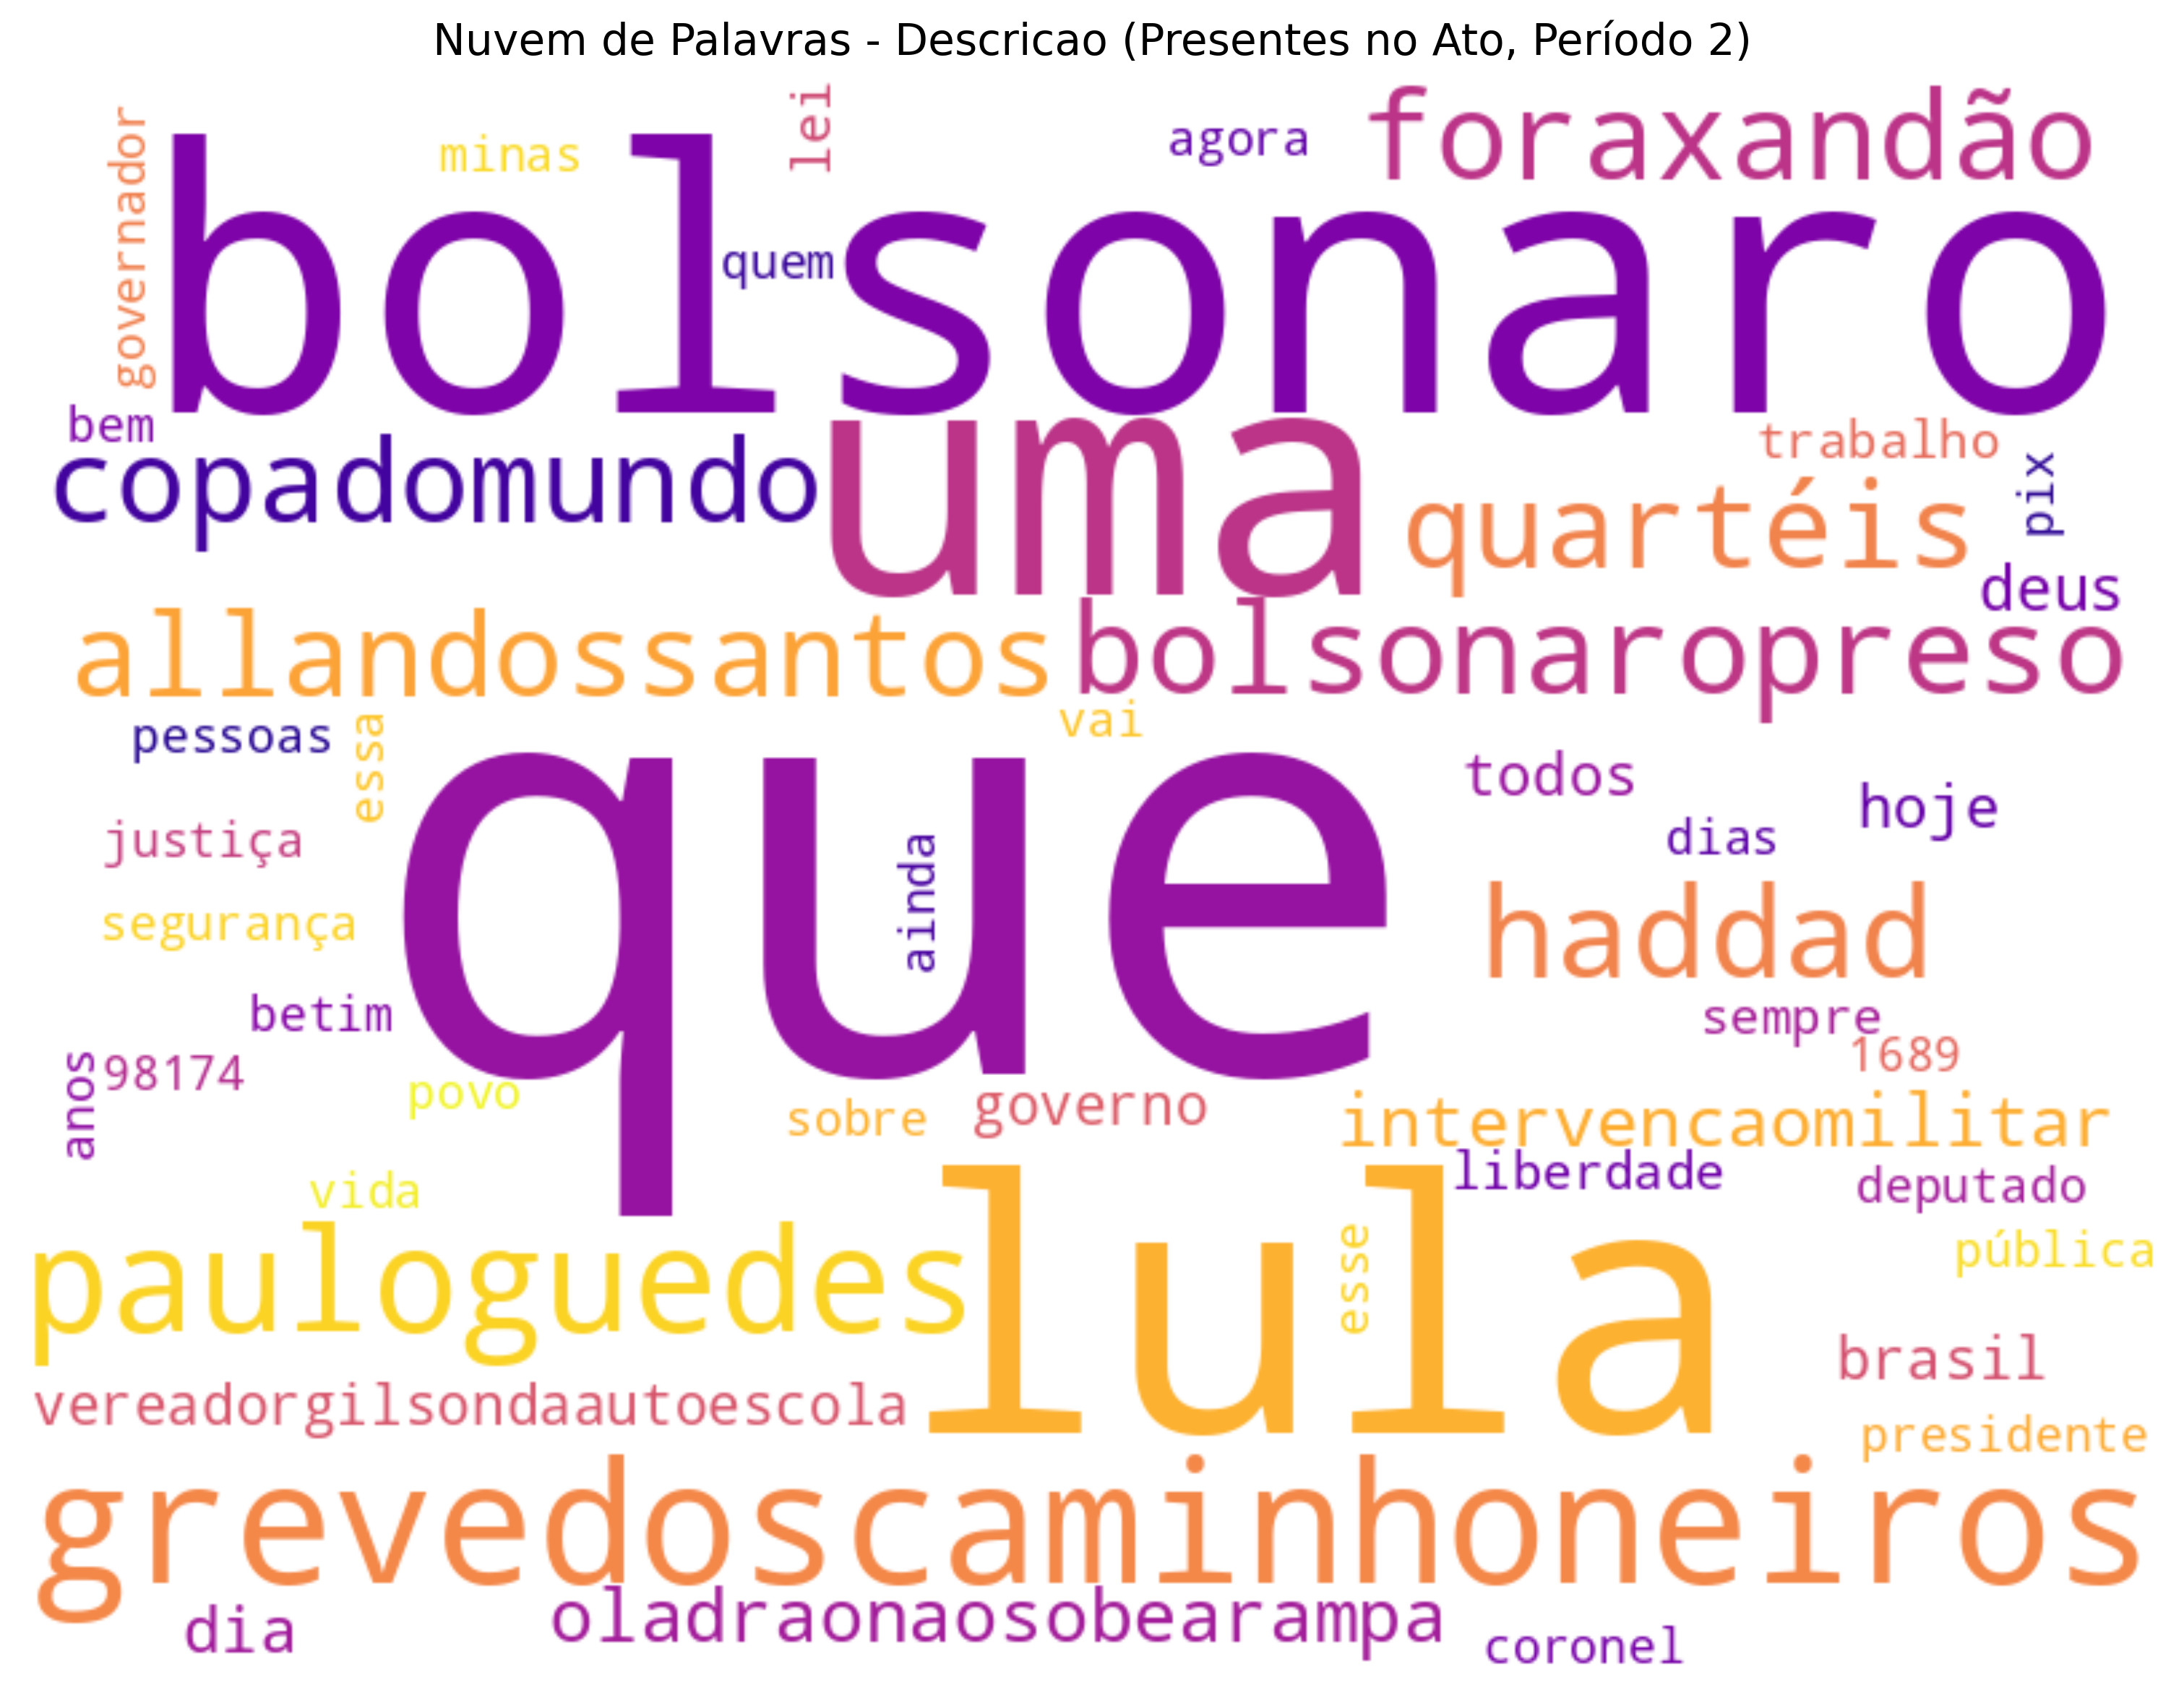
\includegraphics[width=0.8\textwidth]{figura23_nuvem_presentes_desc_periodo2.png}
\caption{Nuvem de palavras - Descrições das pessoas presentes no ato (Período 2: 09/01/2023 a 10/04/2023).}
\label{fig:figura23}
\end{figure}

\begin{figure}[h]
\centering
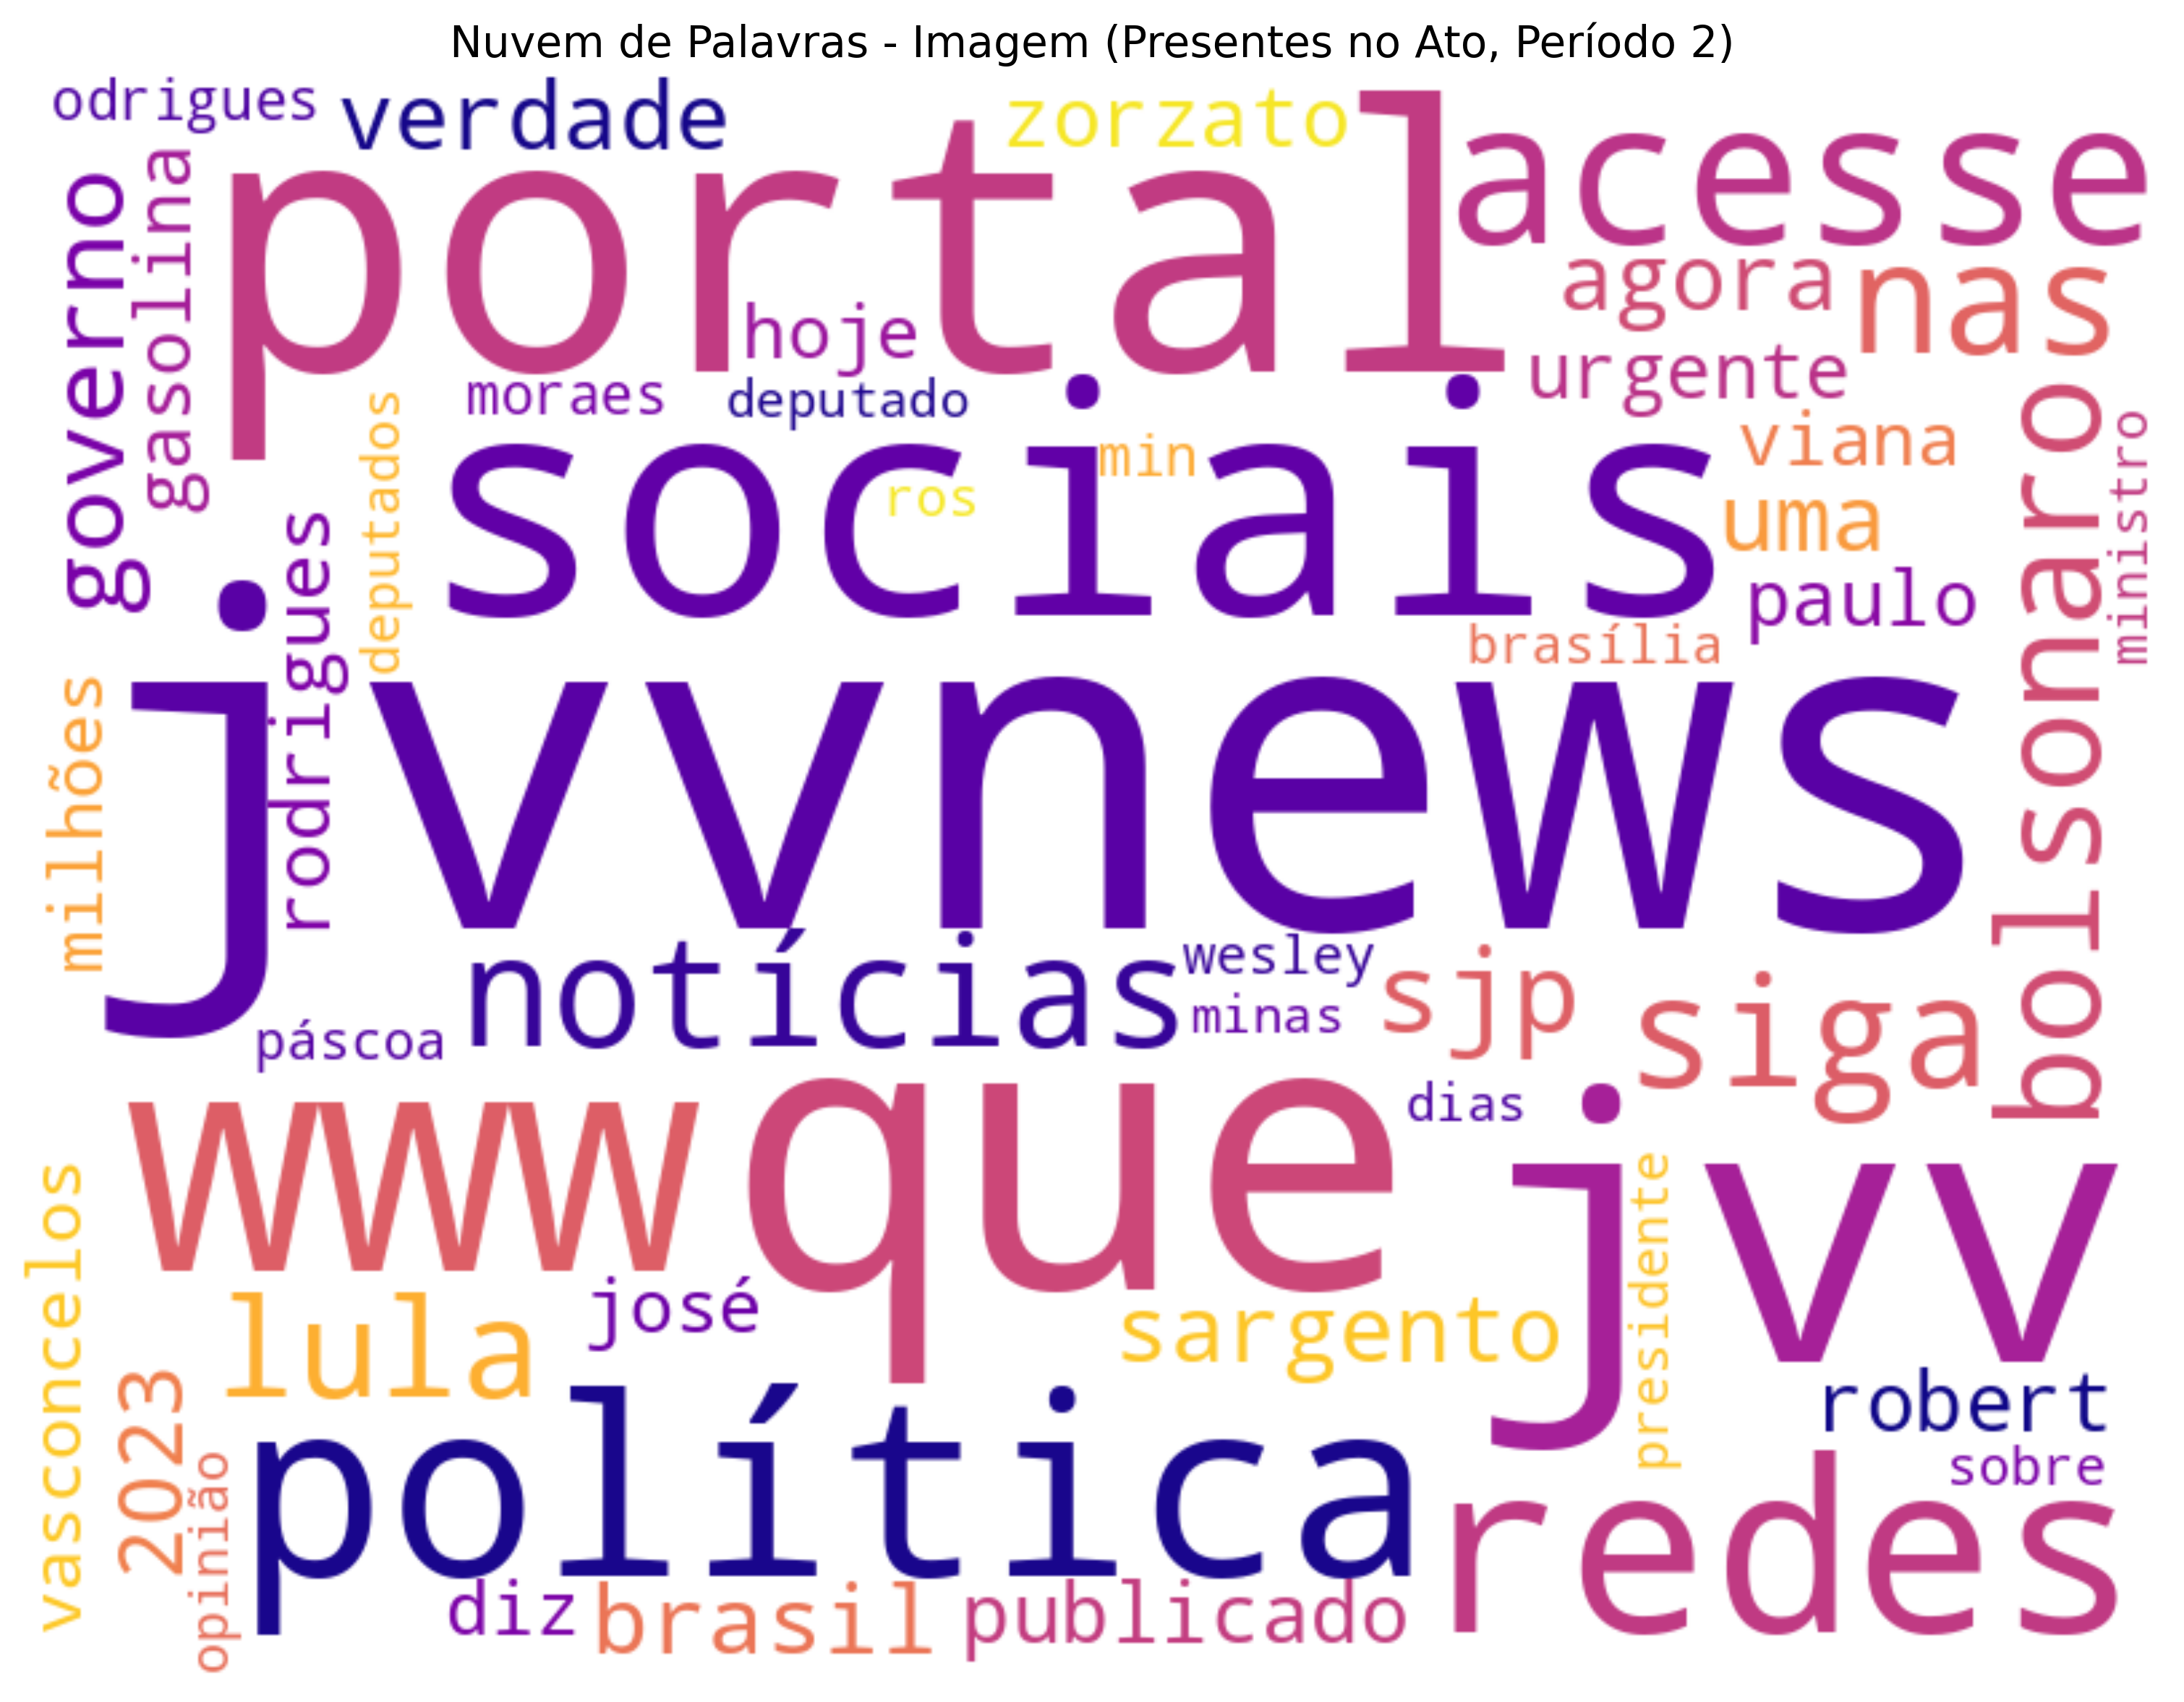
\includegraphics[width=0.8\textwidth]{figura24_nuvem_presentes_img_periodo2.png}
\caption{Nuvem de palavras - Texto das imagens das pessoas presentes no ato (Período 2: 09/01/2023 a 10/04/2023).}
\label{fig:figura24}
\end{figure}

\section{Resultados}

\subsection{Análise de sentimentos}

\subsubsection{Diariamente}

Com esta análise, foi usada a biblioteca \textit{Vader Sentiment}, para analisar se o sentimento dos posts eram positivos ou negativos, com base nos campos de descrição e do campo e de texto das imagens.

\begin{figure}[h]
\centering
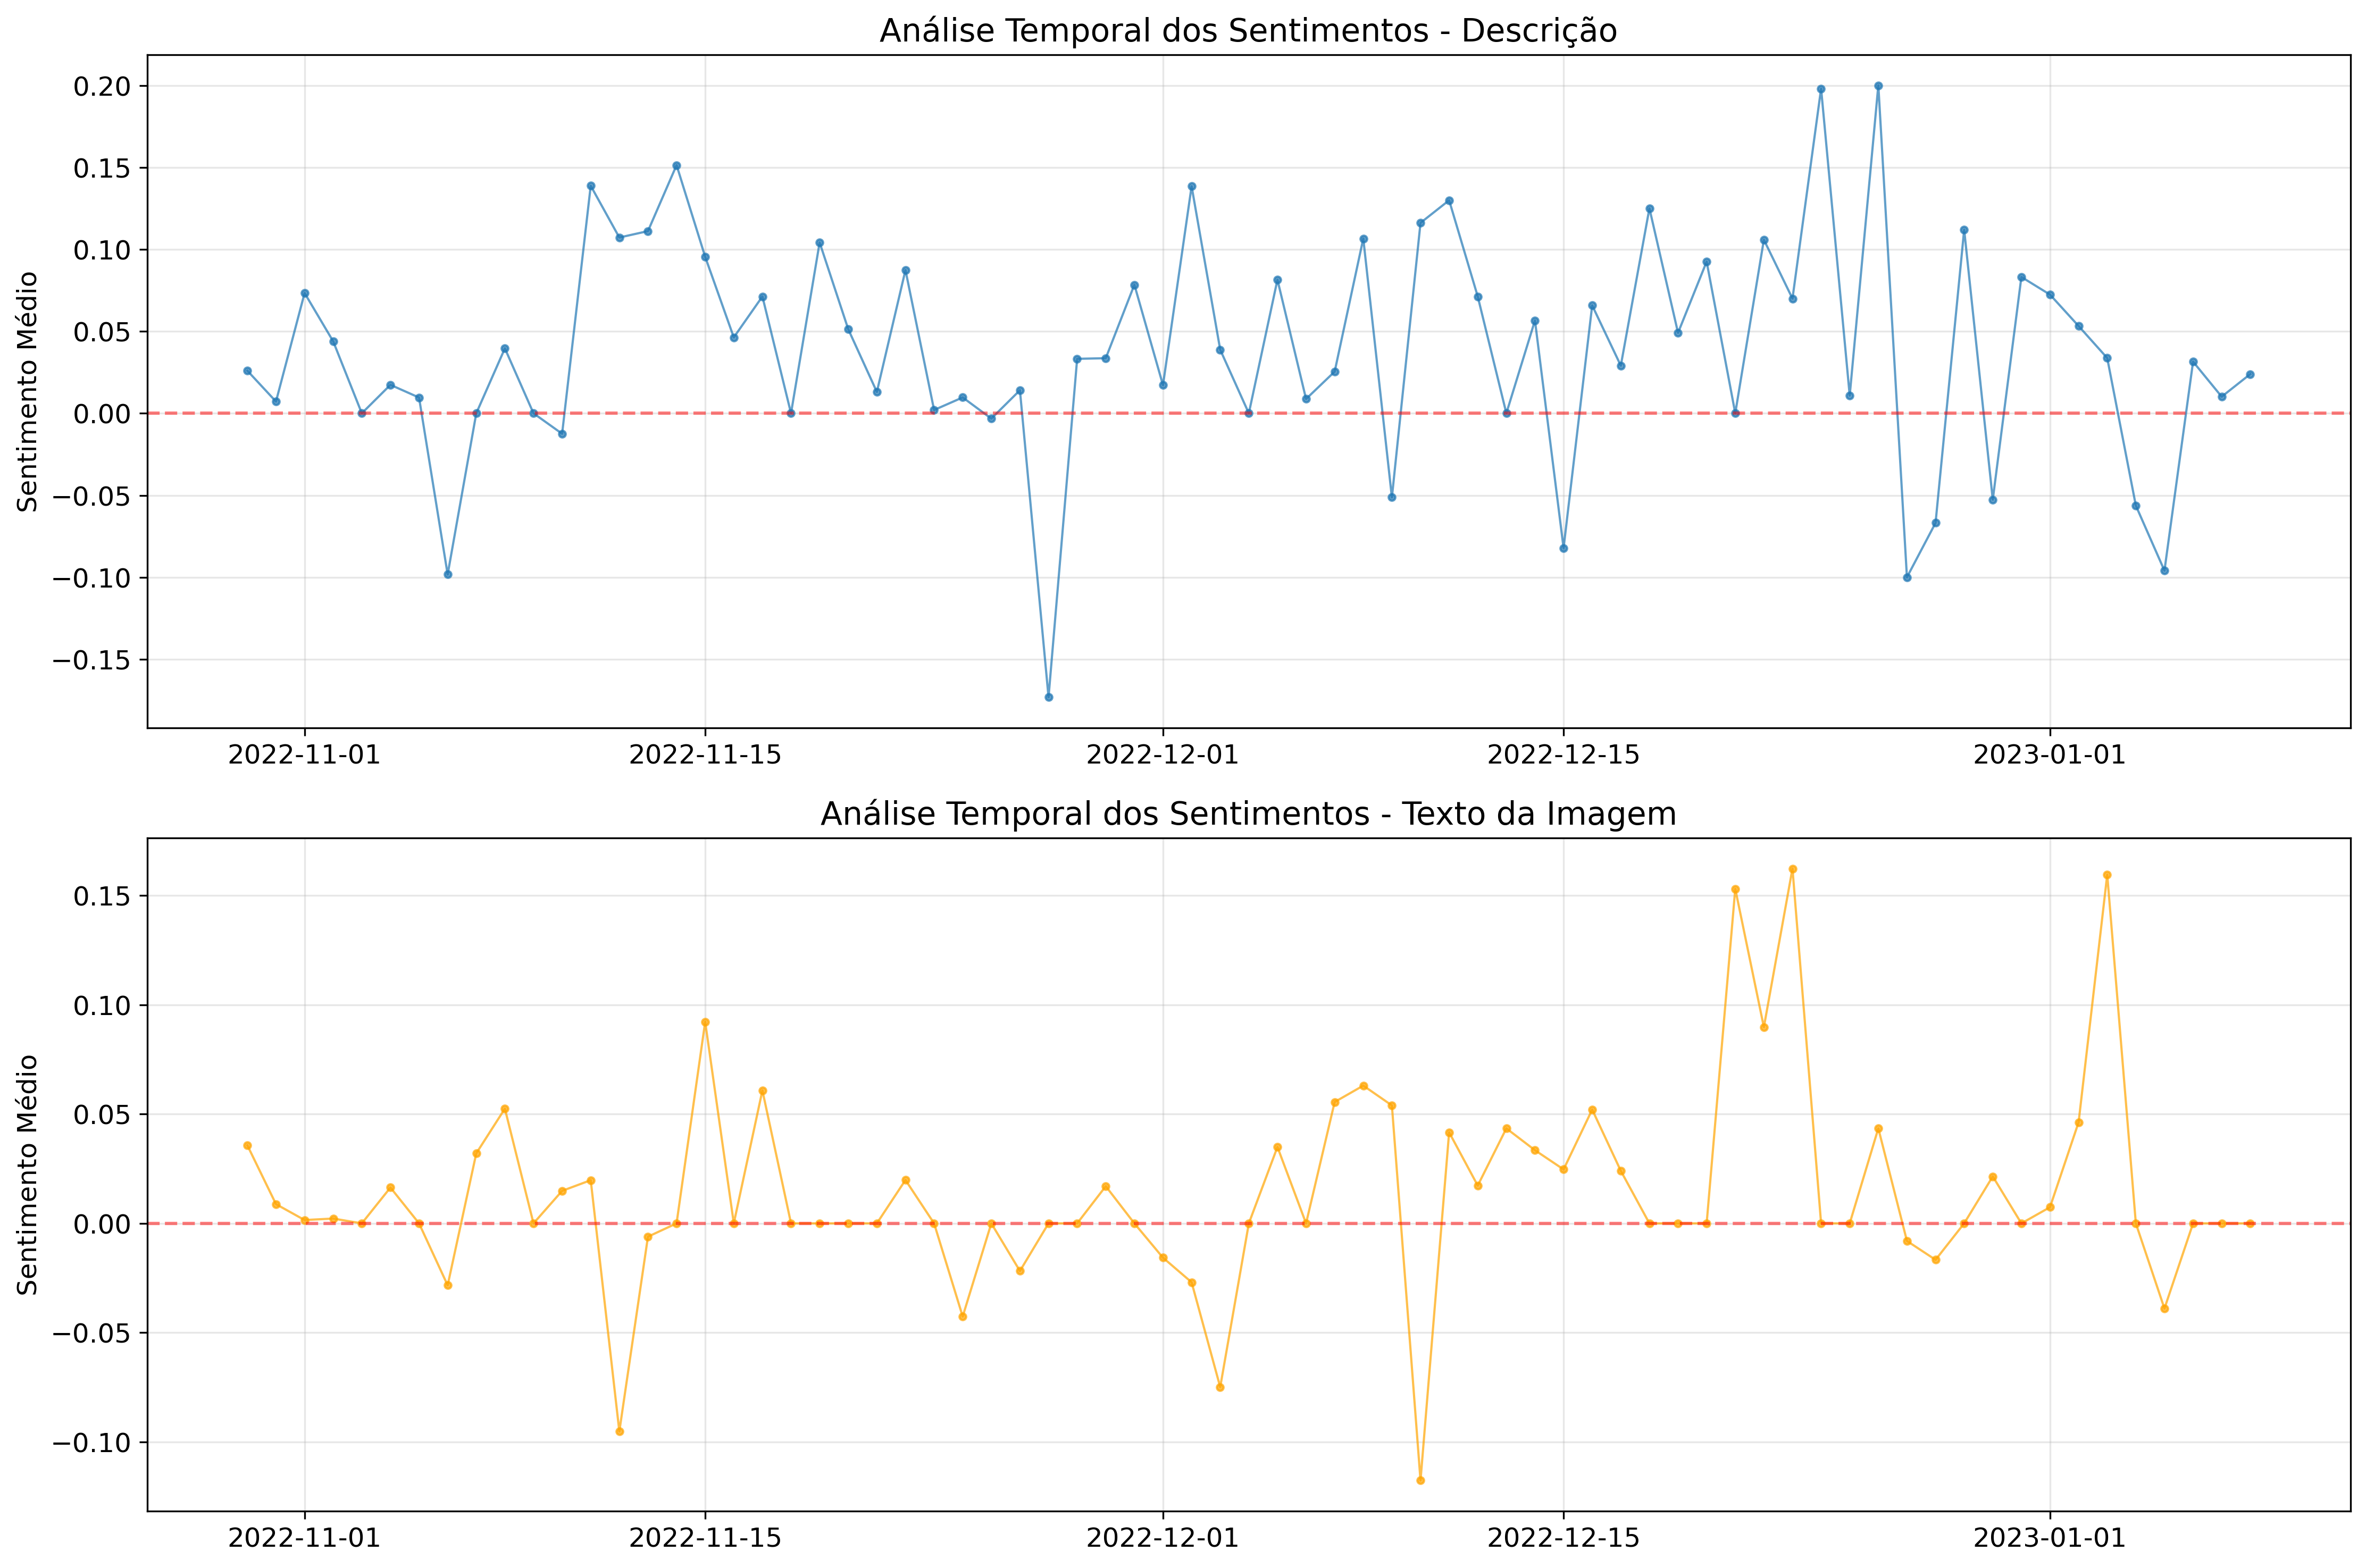
\includegraphics[width=0.8\textwidth]{figura1_sentimentos_verificadas_periodo1.png}
\caption{Análise diária dos sentimentos das pessoas verificadas no período 1 (30/10/2022 a 08/01/2023).}
\label{fig:figura1}
\end{figure}

\begin{figure}[h]
\centering
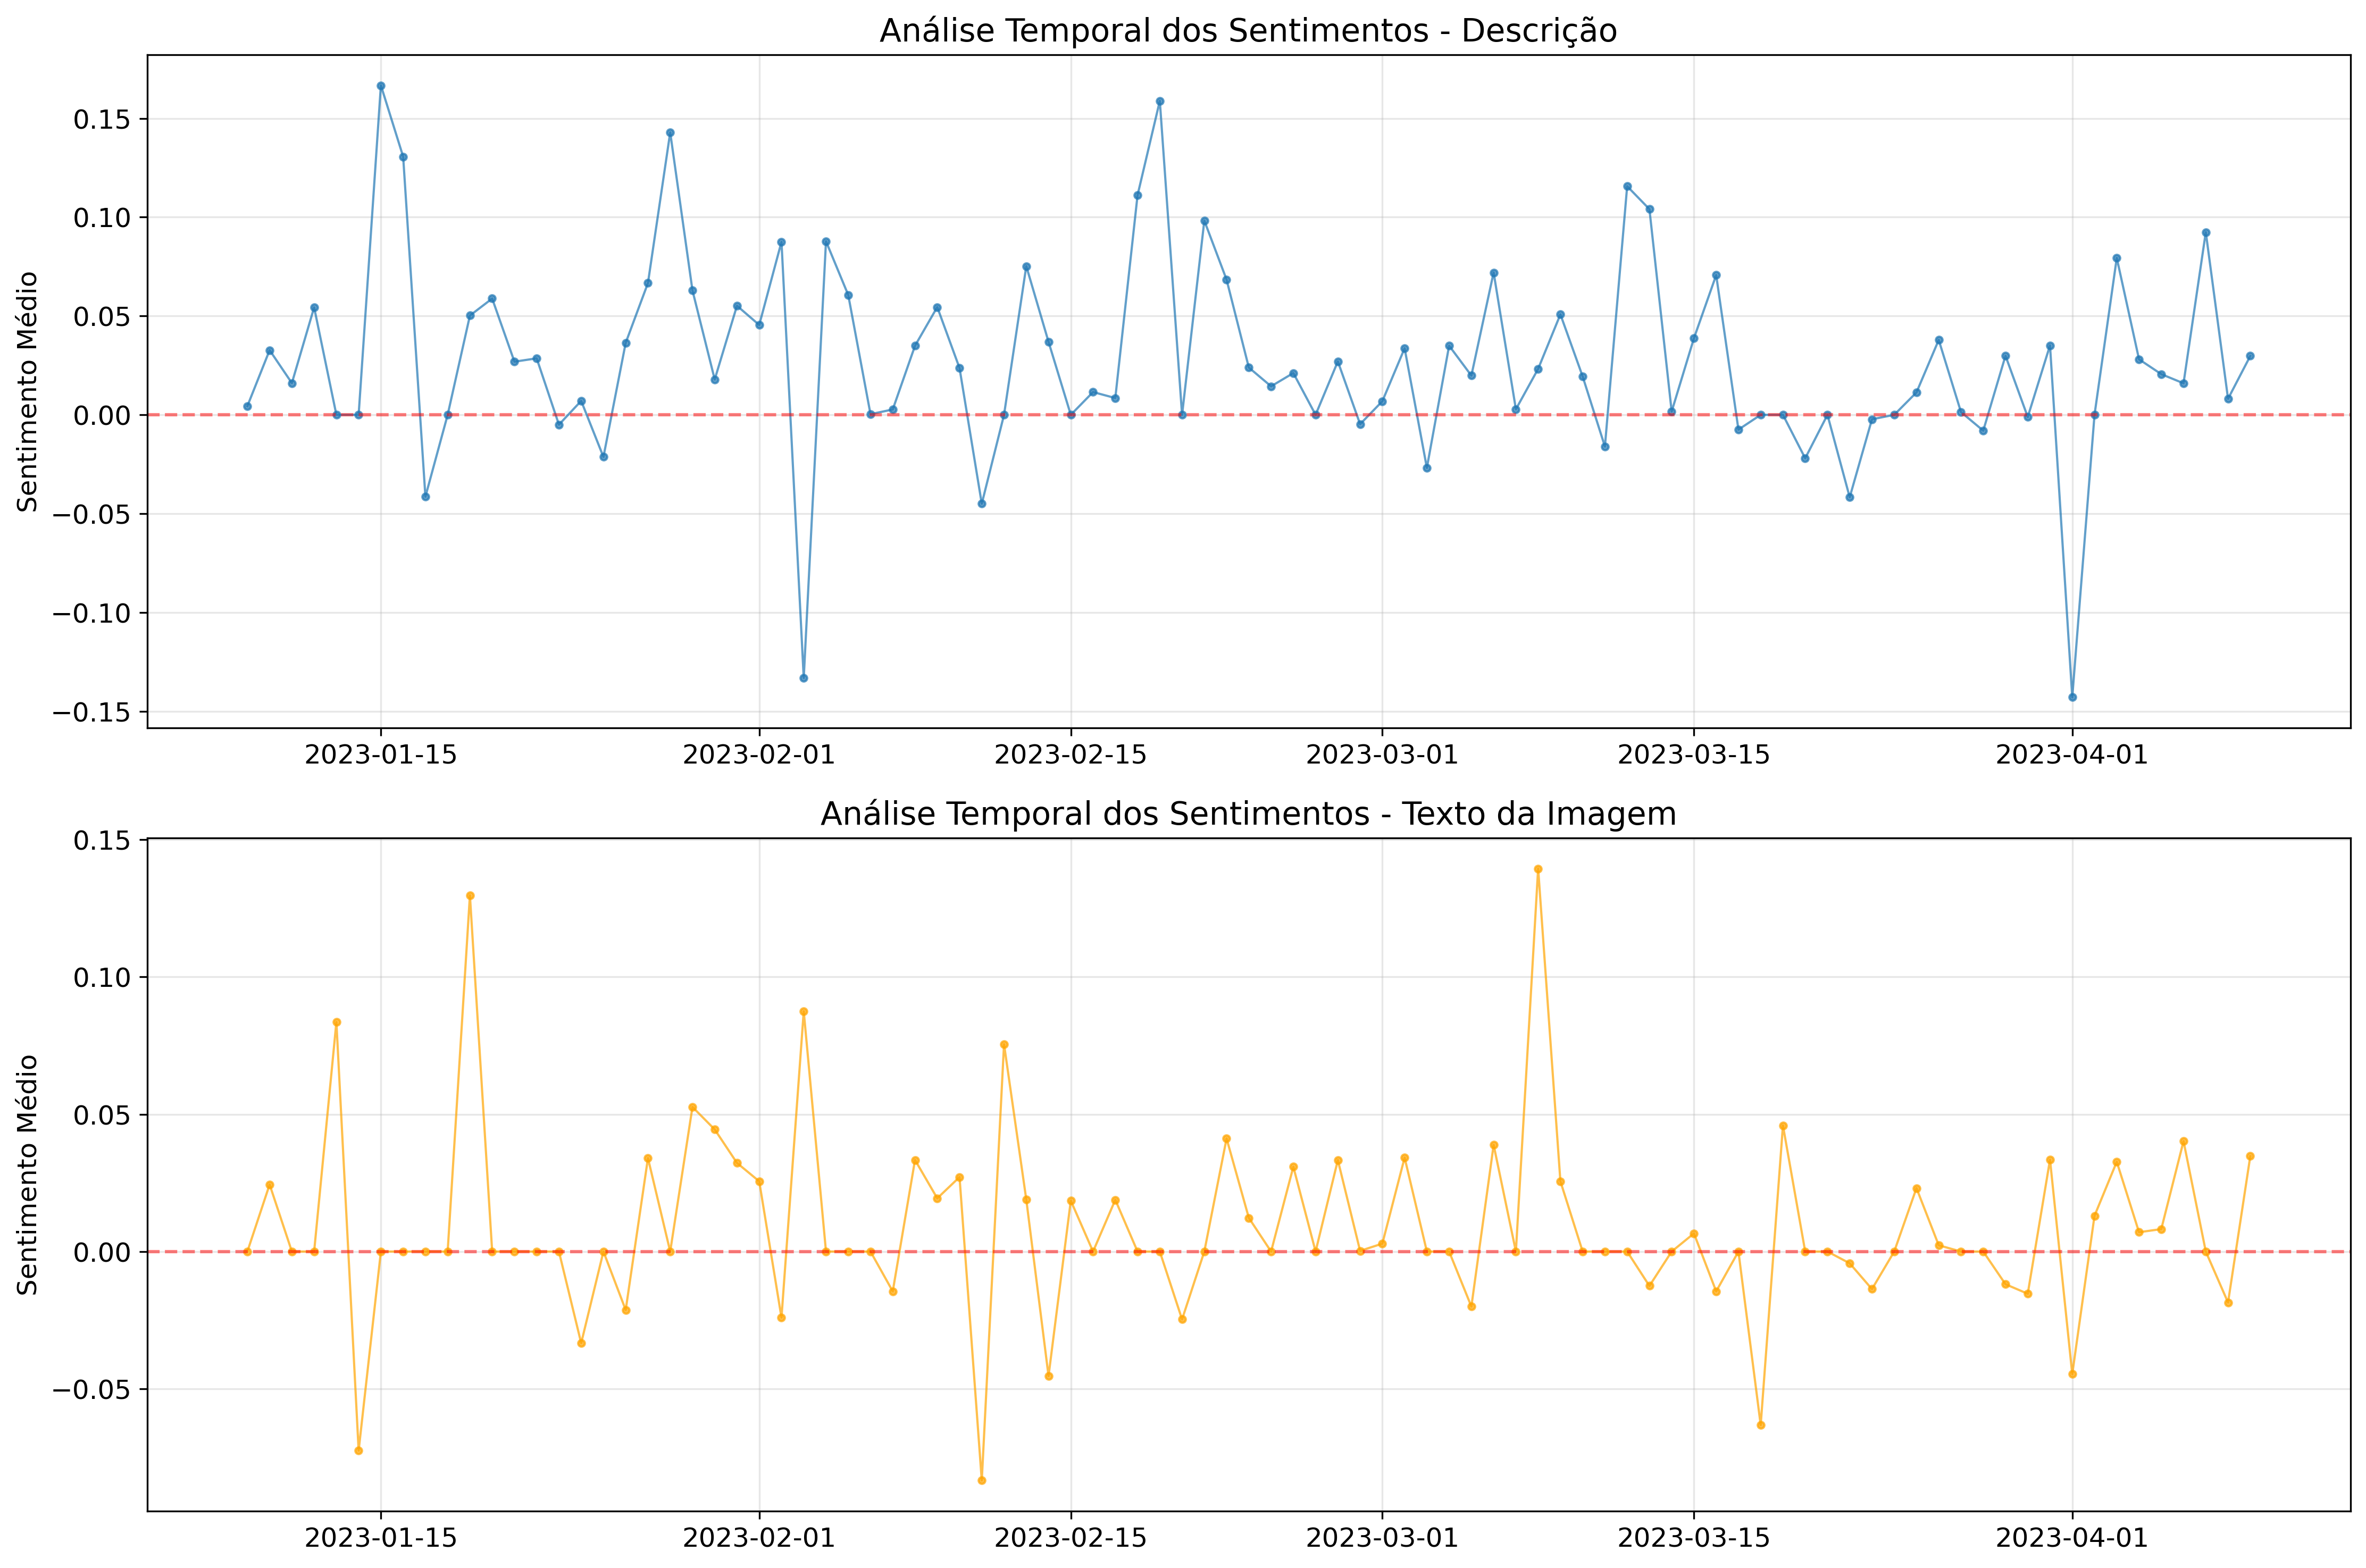
\includegraphics[width=0.8\textwidth]{figura2_sentimentos_verificadas_periodo2.png}
\caption{Análise diária dos sentimentos das pessoas verificadas no período 2 (09/01/2023 a 10/04/2023).}
\label{fig:figura2}
\end{figure}

\begin{figure}[h]
\centering
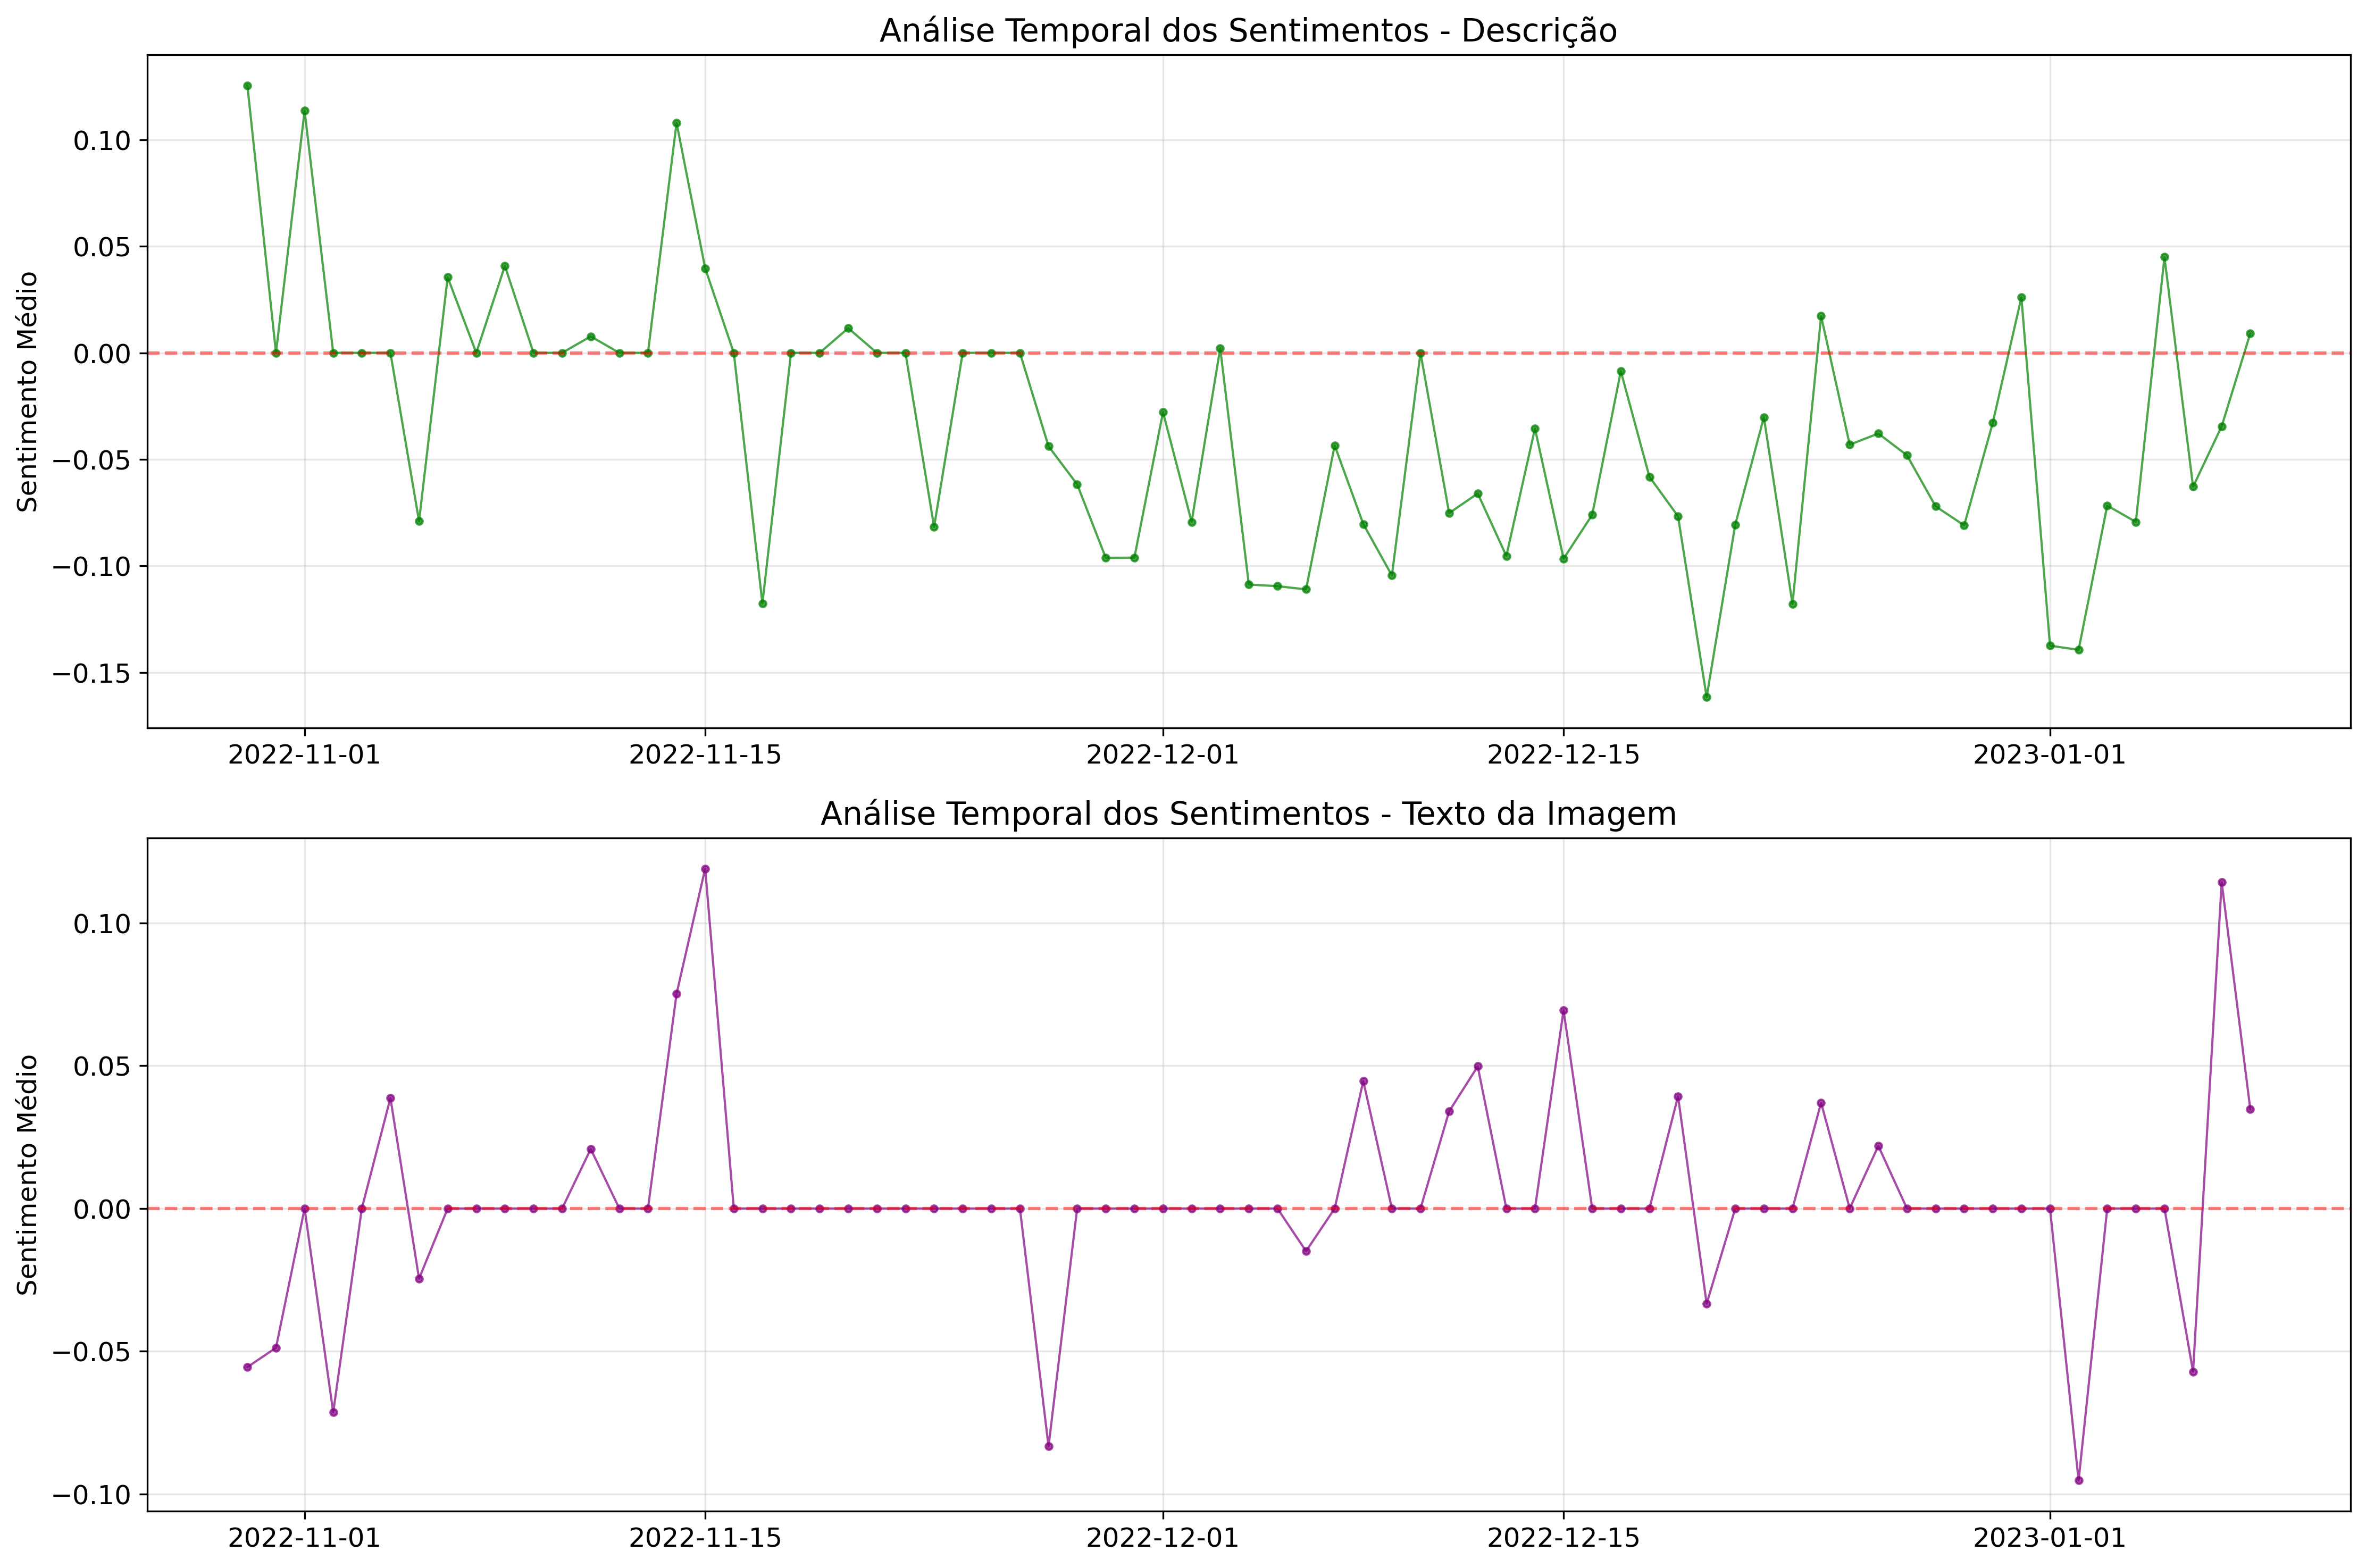
\includegraphics[width=0.8\textwidth]{figura3_sentimentos_presentes_periodo1.png}
\caption{Análise diária dos sentimentos das pessoas presentes no ato no período 1 (30/10/2022 a 08/01/2023).}
\label{fig:figura3}
\end{figure}

\begin{figure}[h]
\centering
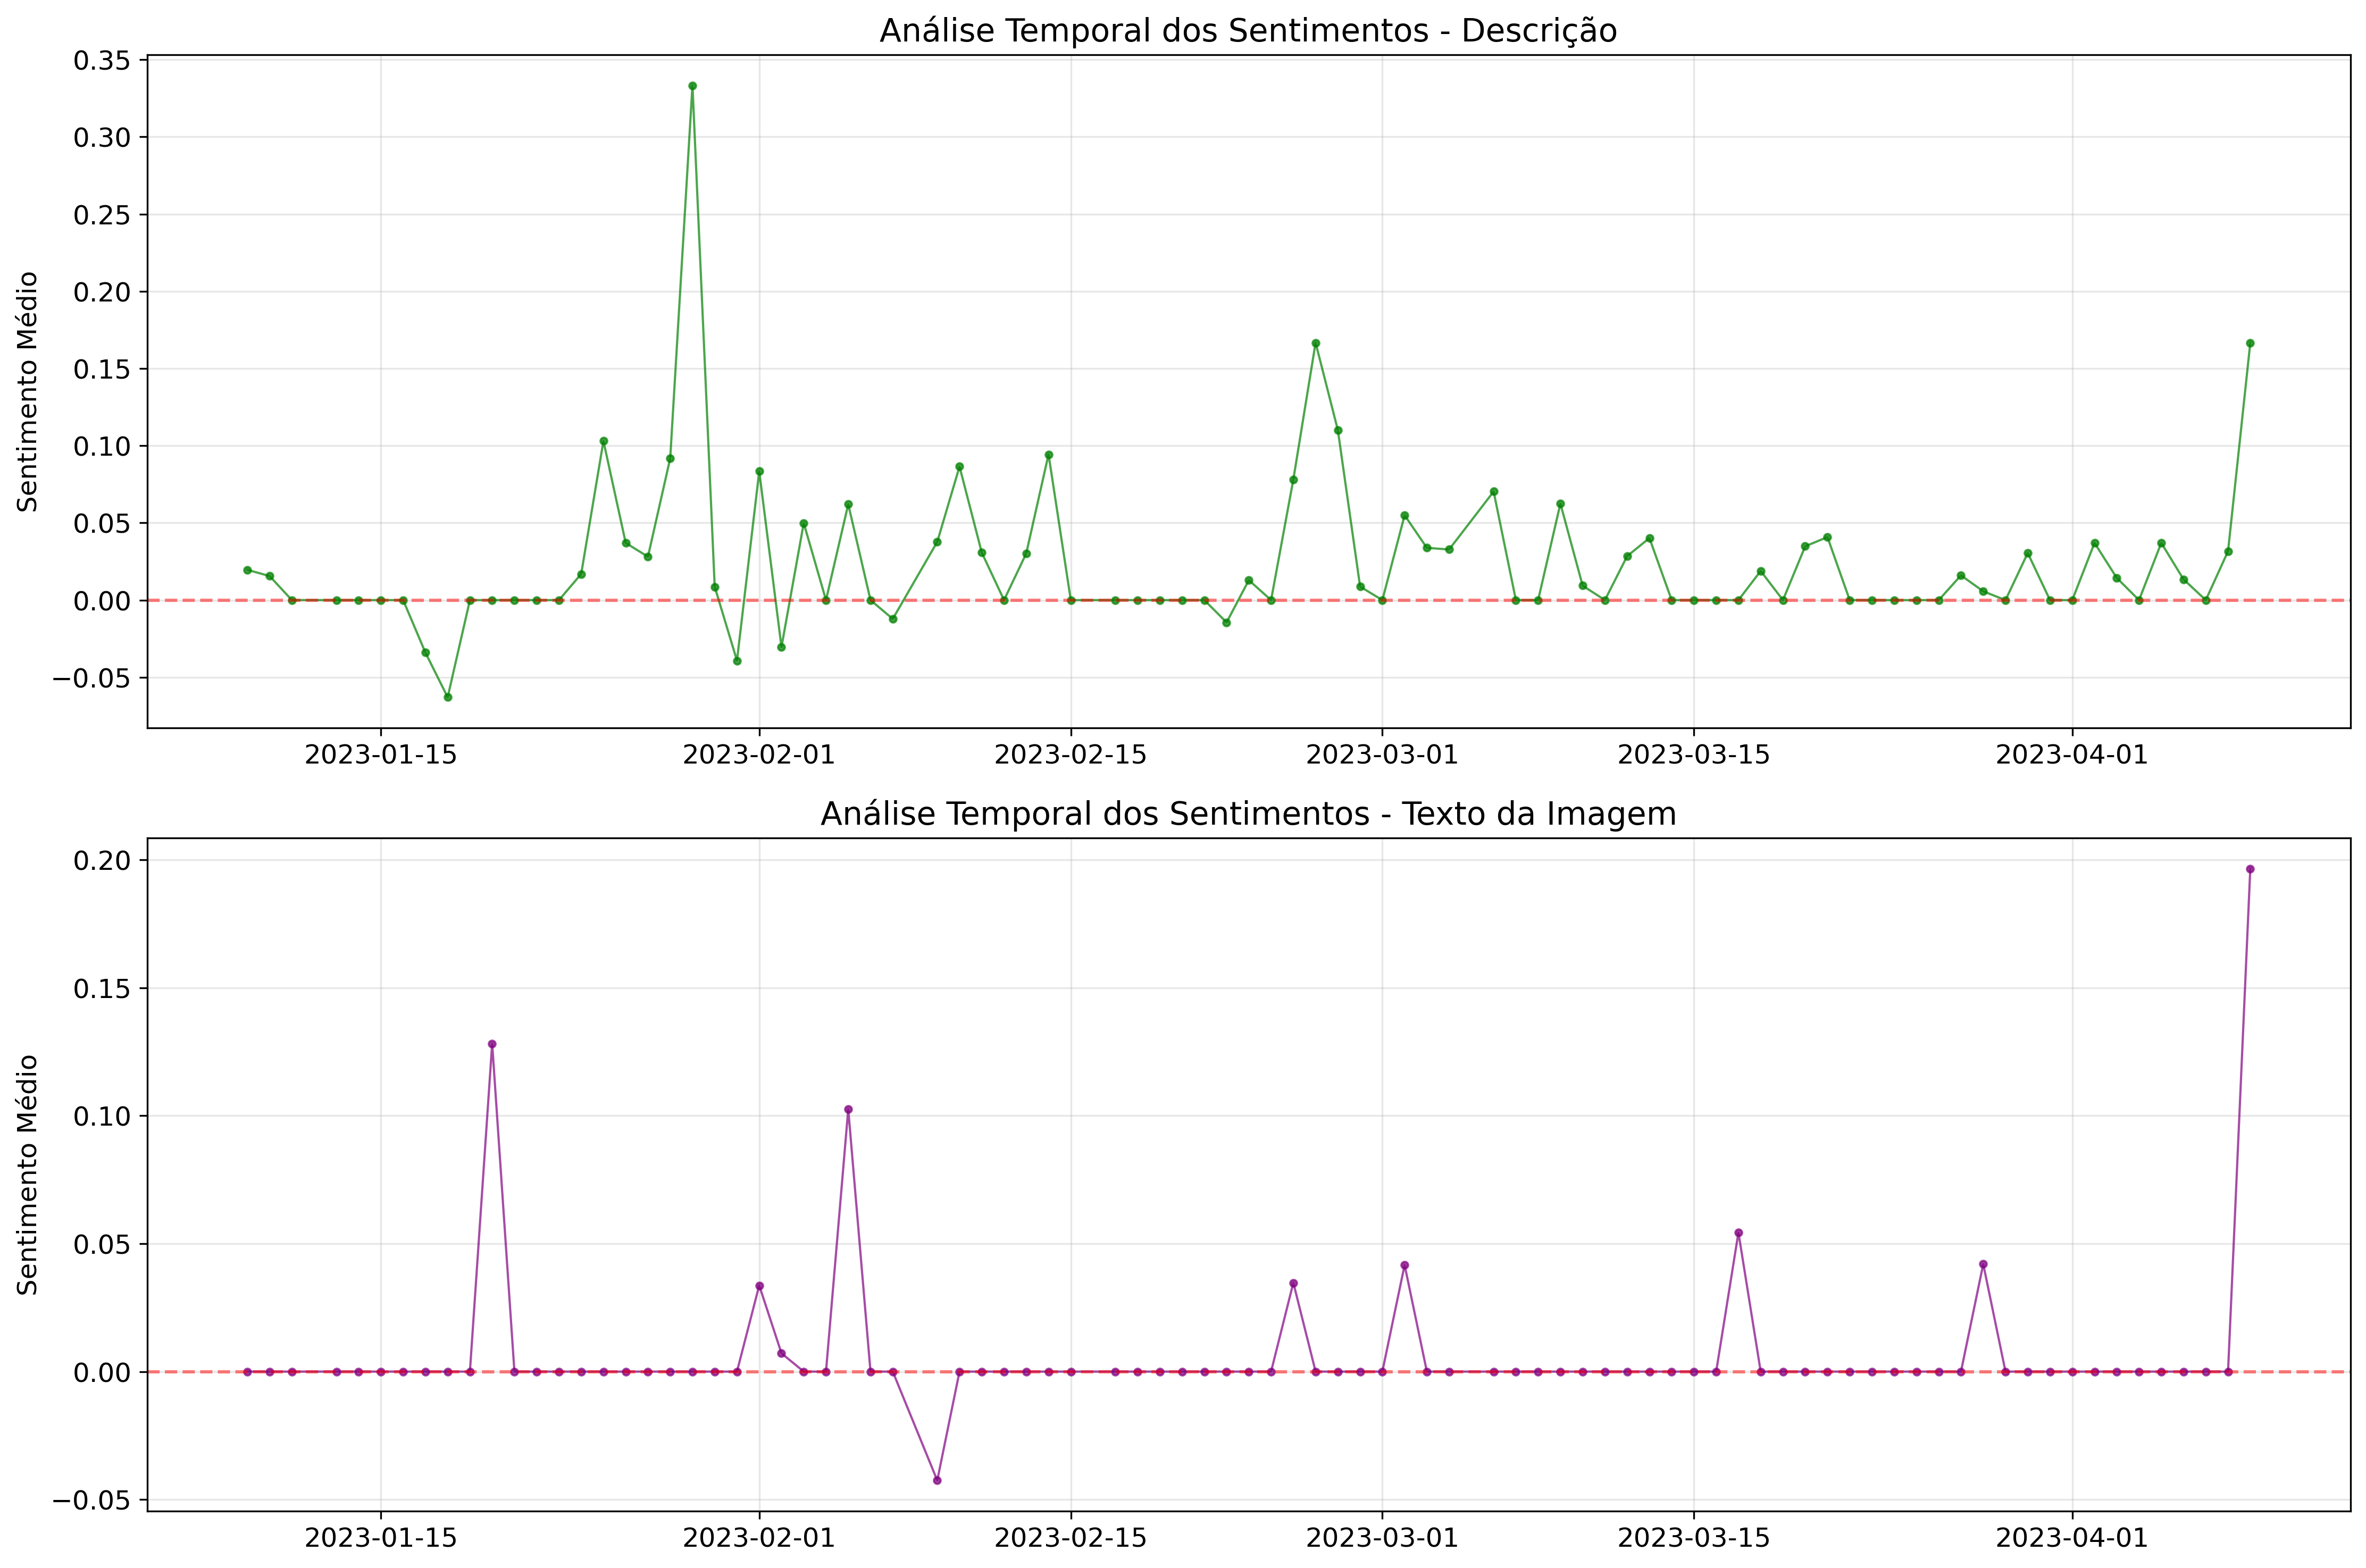
\includegraphics[width=0.8\textwidth]{figura4_sentimentos_presentes_periodo2.png}
\caption{Análise diária dos sentimentos das pessoas presentes no ato no período 2 (09/01/2023 a 10/04/2023).}
\label{fig:figura4}
\end{figure}

As análises de sentimento diárias, demonstradas nas figuras 1, 2, 3 e 4, mostraram grande turbulência nos sentimentos dos usuários, ambas figuras públicas e os presentes no ato, indo geralmente de -0.3 (negativo) até 0.4 (positivo), ocasionalmente chegando a picos mais elevados. É possível observar, comparando as figuras 1 e 2, que no período após o dia 8, a turbulência das emoções foi mais pronunciada, e algo semelhante também ocorre comparando as figuras 3 e 4, ocorrendo uma leve tendência a sentimentos mais negativos no período após o dia 8.

\subsubsection{Mensalmente}

\begin{figure}[h]
\centering
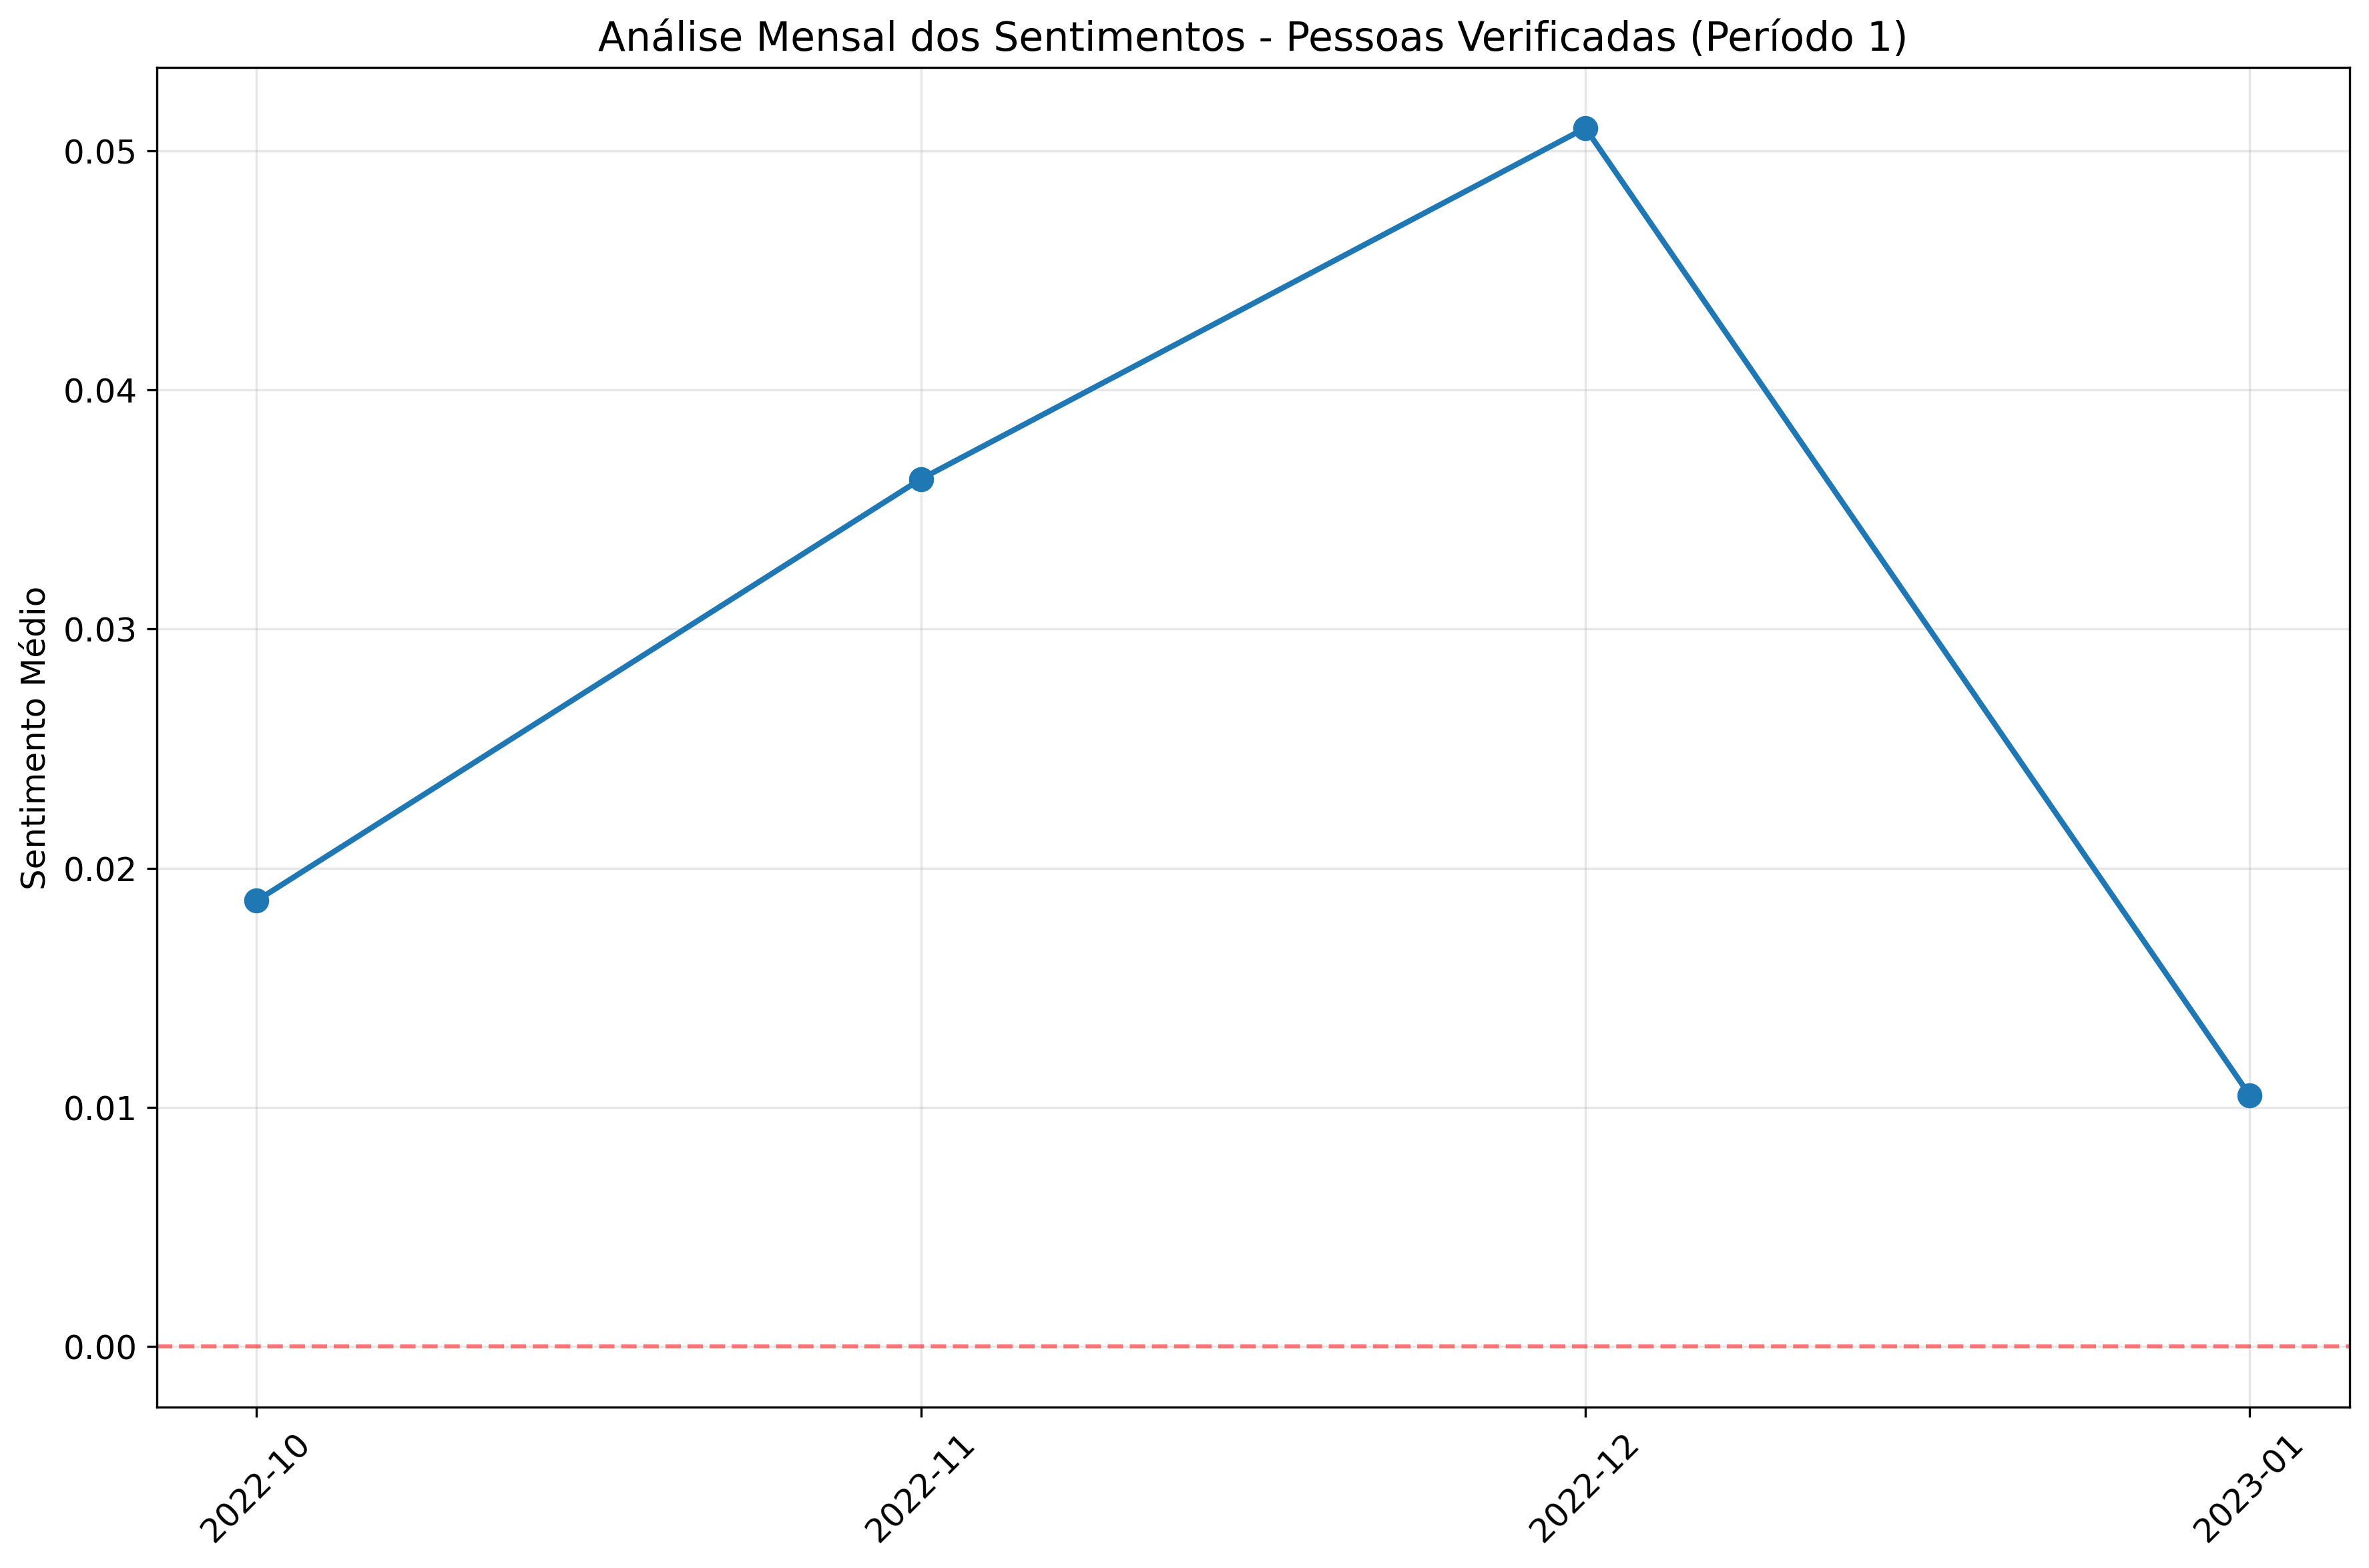
\includegraphics[width=0.8\textwidth]{figura5_sentimentos_verificadas_mensal_periodo1.png}
\caption{Análise mensal dos sentimentos das pessoas verificadas no período 1 (30/10/2022 a 08/01/2023).}
\label{fig:figura5}
\end{figure}

\begin{figure}[h]
\centering
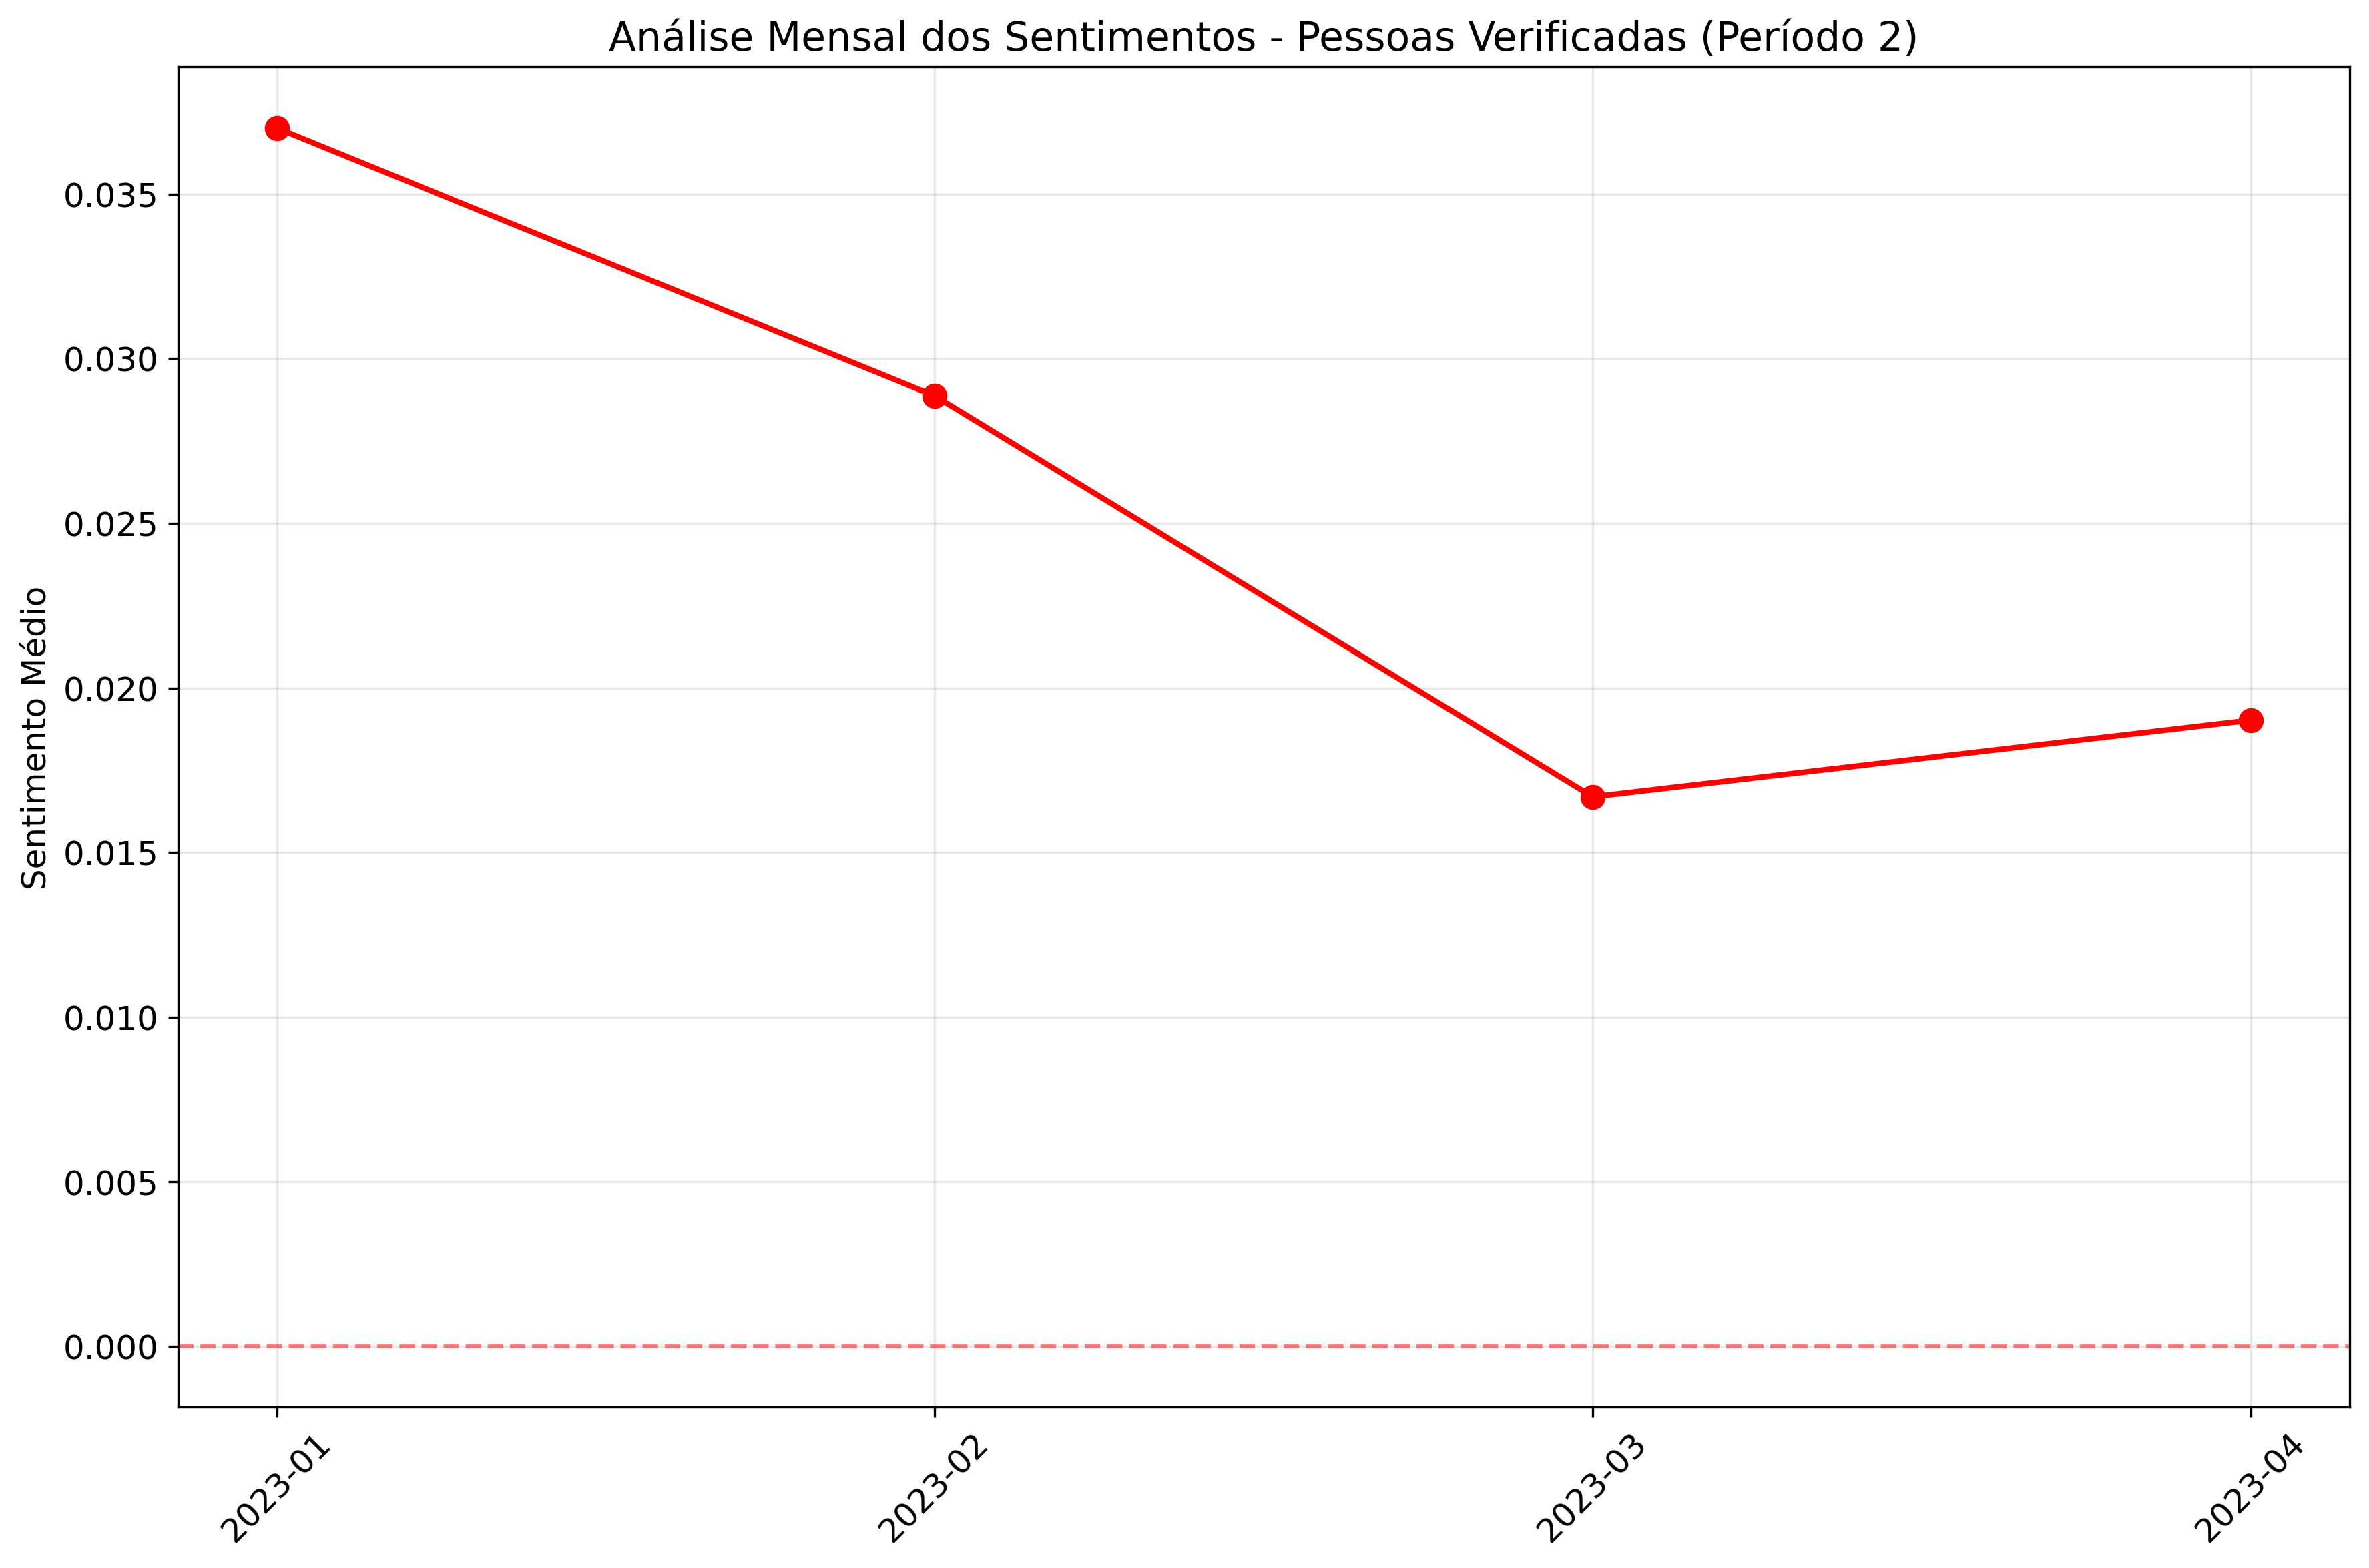
\includegraphics[width=0.8\textwidth]{figura6_sentimentos_verificadas_mensal_periodo2.png}
\caption{Análise mensal dos sentimentos das pessoas verificadas no período 2 (09/01/2023 a 10/04/2023).}
\label{fig:figura6}
\end{figure}

\begin{figure}[h]
\centering
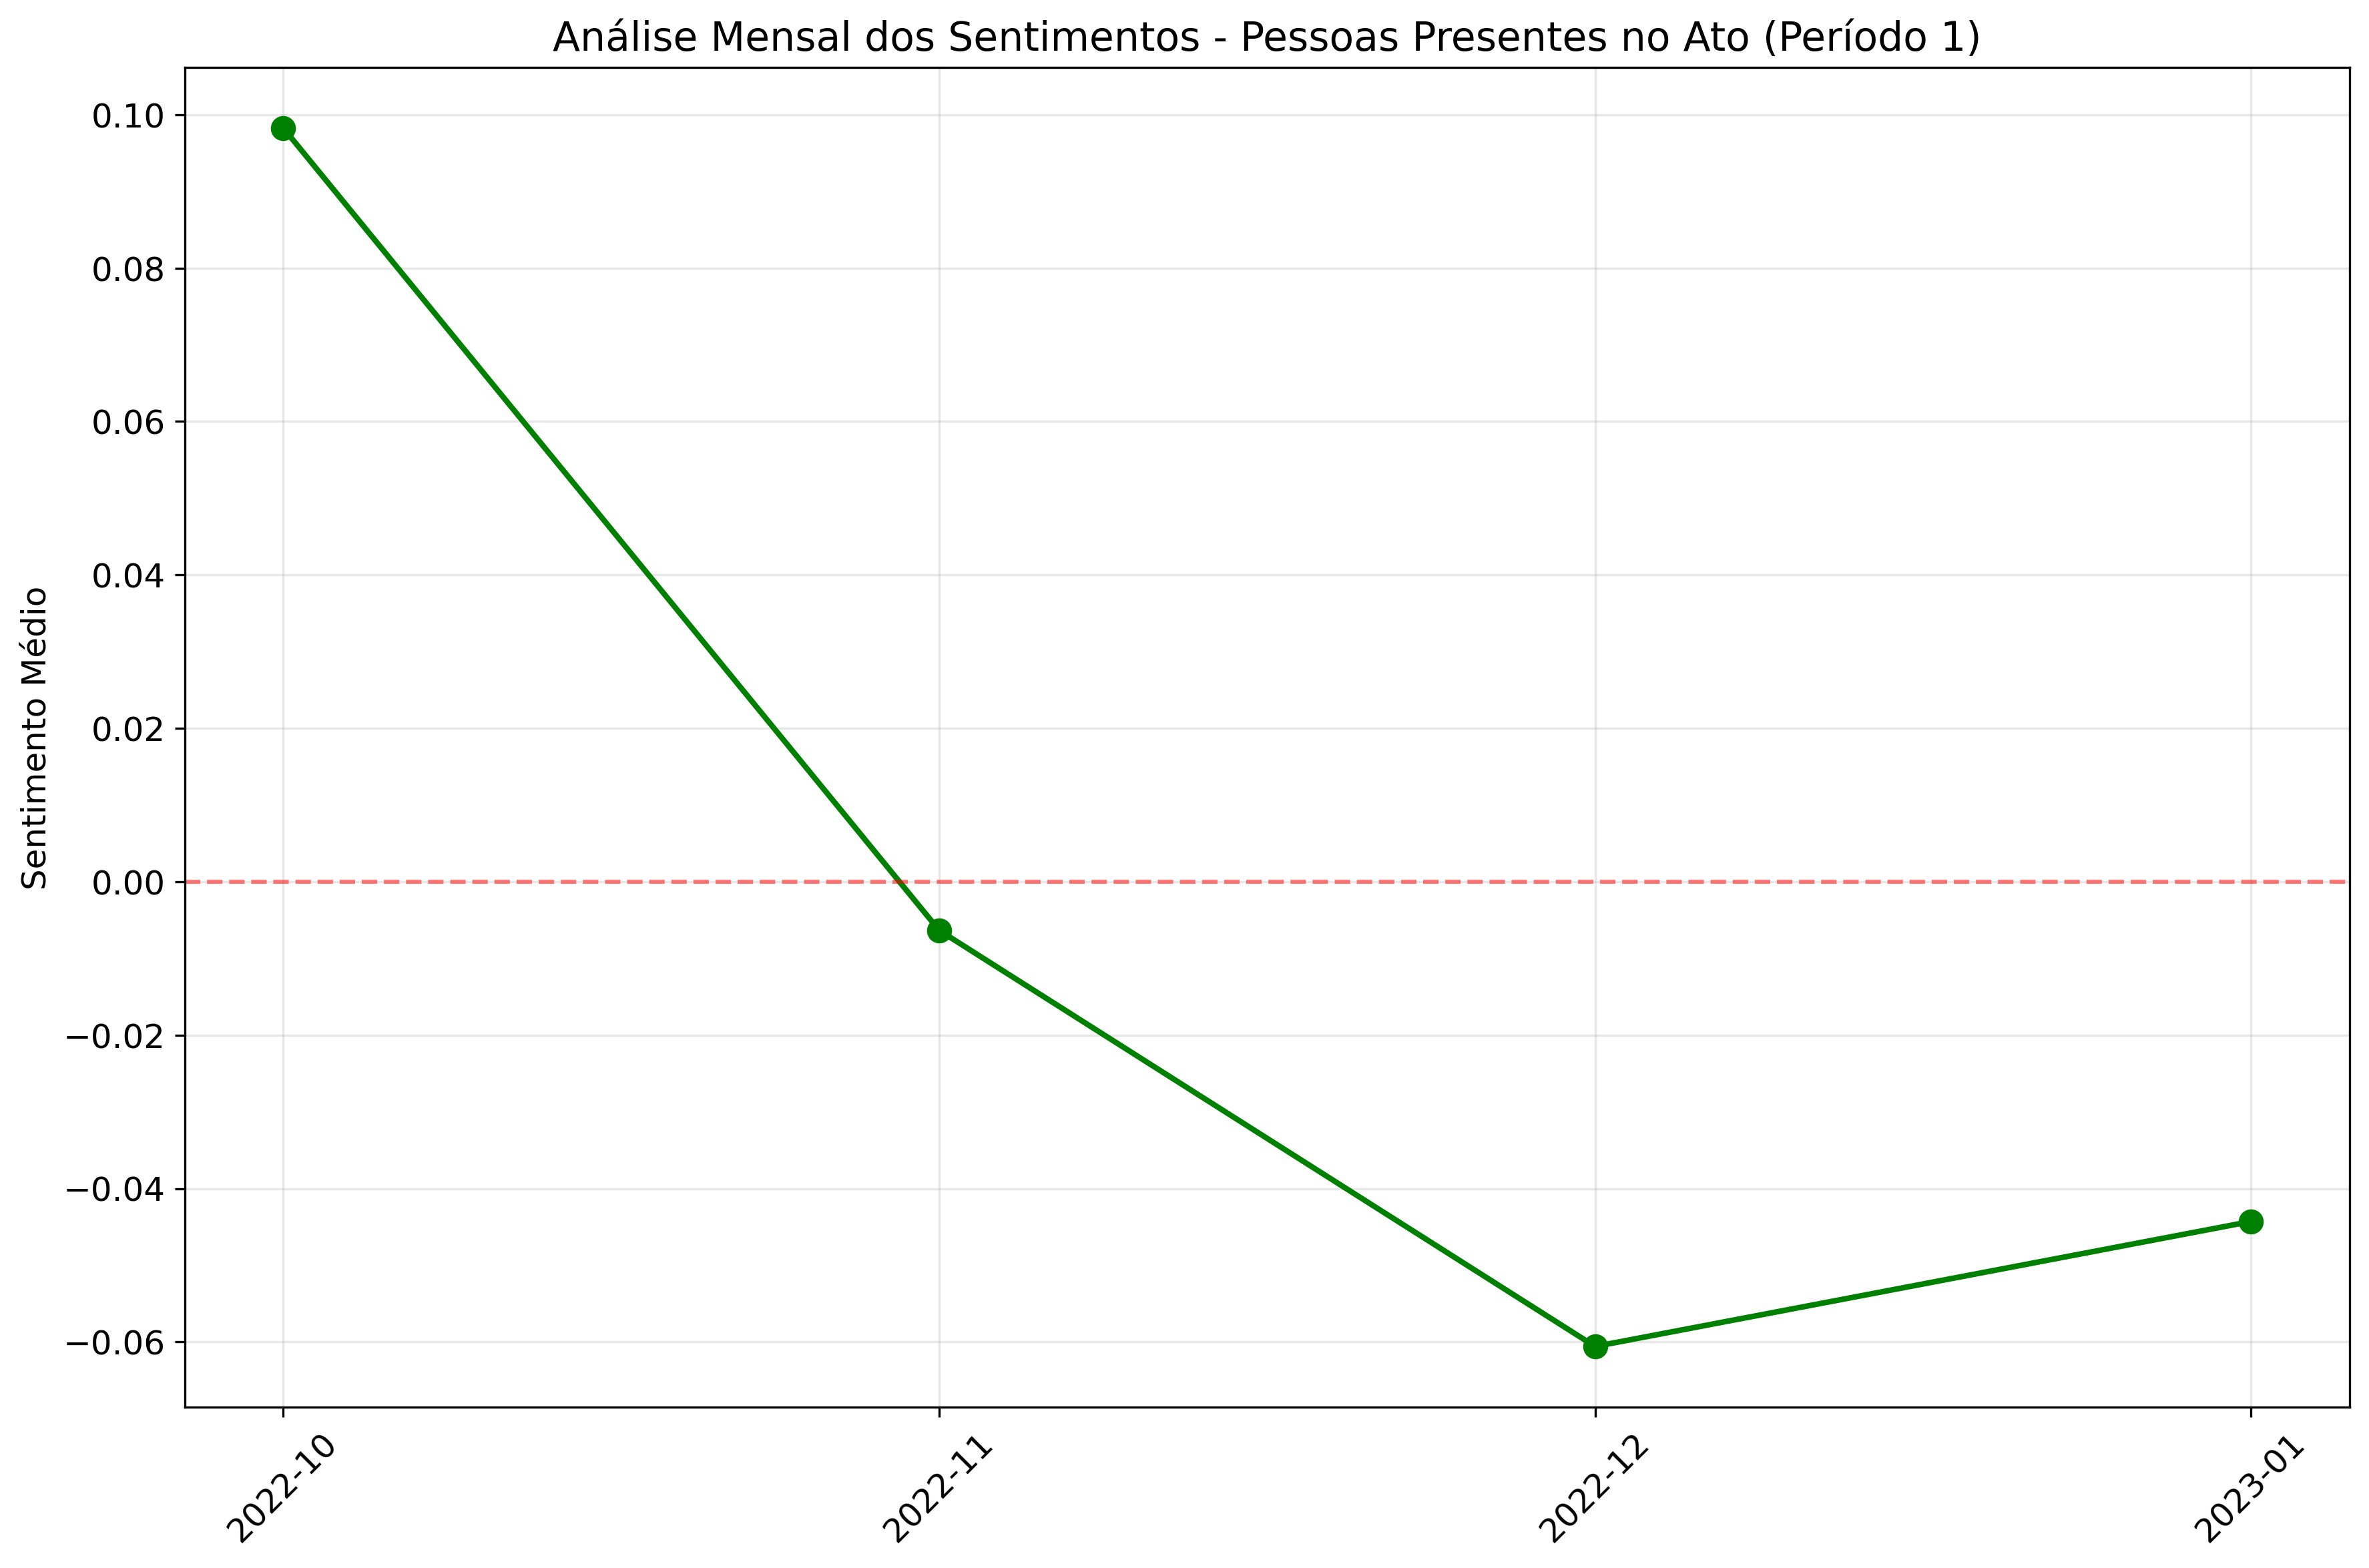
\includegraphics[width=0.8\textwidth]{figura7_sentimentos_presentes_mensal_periodo1.png}
\caption{Análise mensal dos sentimentos das pessoas presentes no ato no período 1 (30/10/2022 a 08/01/2023).}
\label{fig:figura7}
\end{figure}

\begin{figure}[h]
\centering
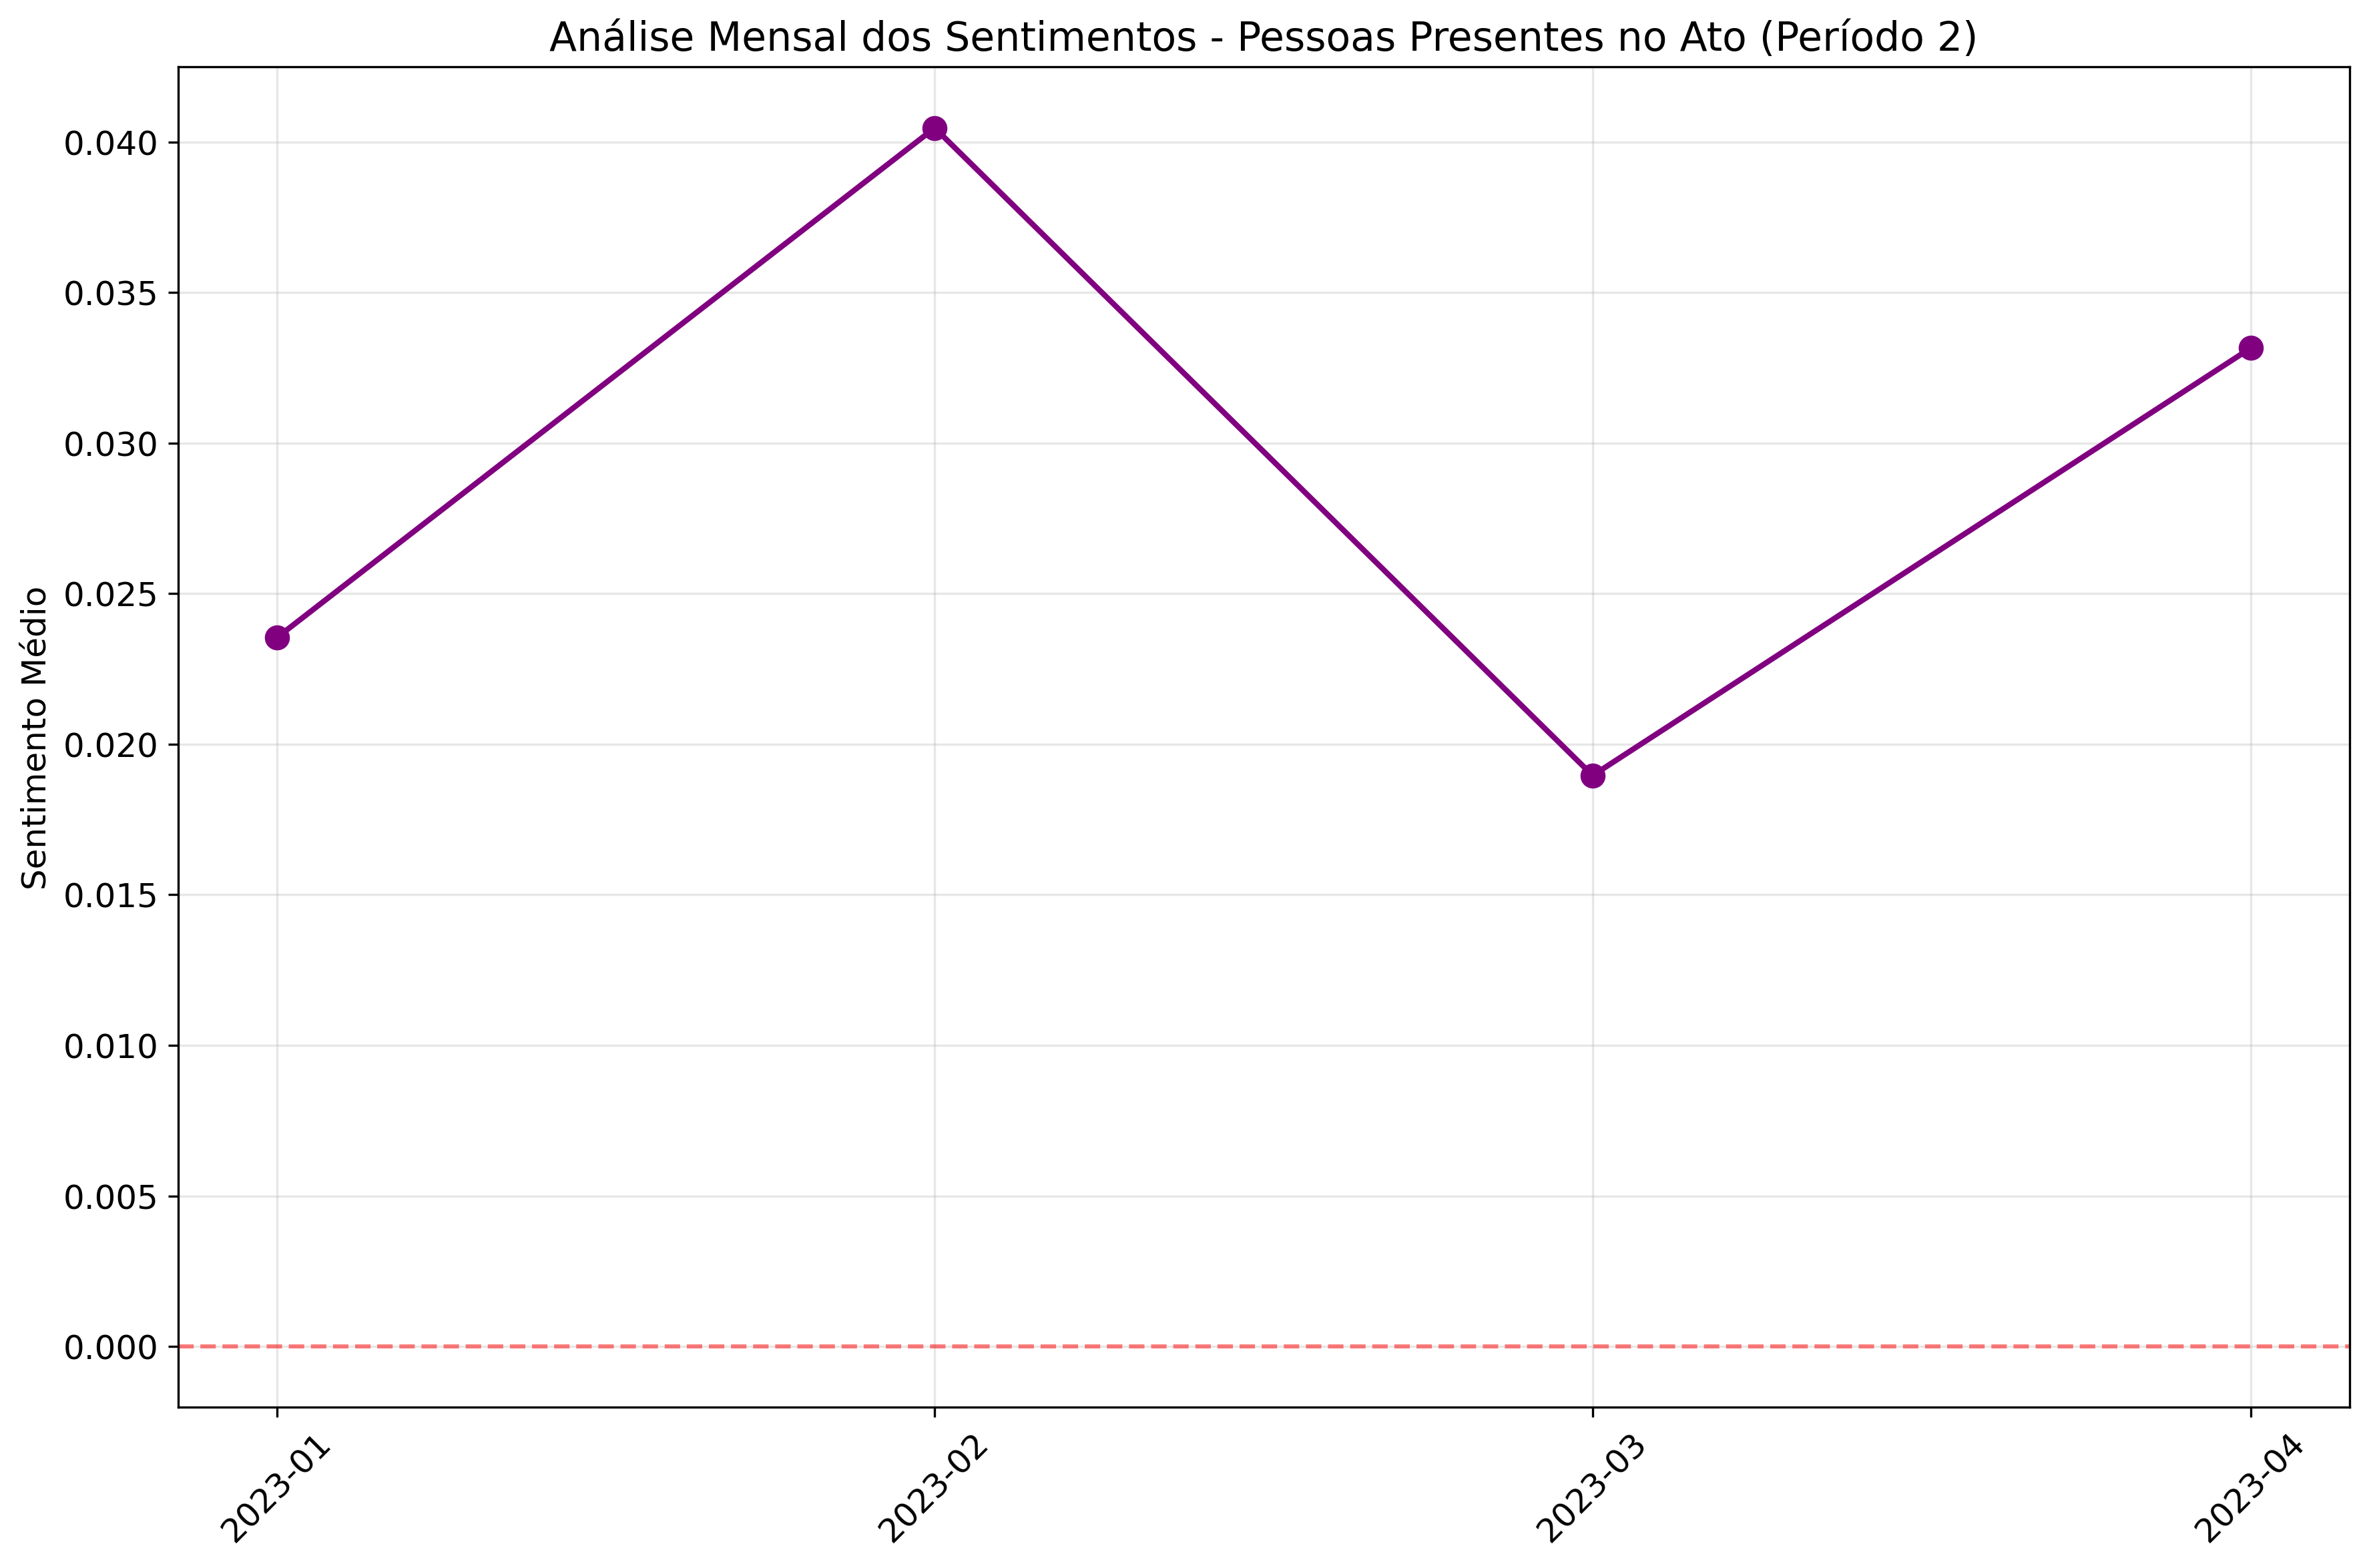
\includegraphics[width=0.8\textwidth]{figura8_sentimentos_presentes_mensal_periodo2.png}
\caption{Análise mensal dos sentimentos das pessoas presentes no ato no período 2 (09/01/2023 a 10/04/2023).}
\label{fig:figura8}
\end{figure}

Observa-se que, no período anterior ao ato, aos sentimentos das pessoas verificadas estava principalmente subindo, enquanto o das presentes no ato estava em declínio. Já no período 2, ambas as pessoas verificadas e presentes no ato tiveram um aumento na positividade. É importante notar a escala dos gráficos, que mostra uma diferença de aproximadamente 10 pontos percentuais para os períodos.

\subsubsection{Divisão de Sentimentos Por Pessoa}

A análise da divisão de sentimentos por pessoa revelou padrões interessantes entre os diferentes grupos de usuários. Para as pessoas verificadas, observou-se que muitas contas, como adrillesjorge, bolsonarosp e flaviobolsonaro, apresentaram maior negatividade nos posts no período após o ato em comparação com o período anterior. Por outro lado, nas postagens dos presentes no ato, a positividade aumentou significativamente no período após o ato, possivelmente refletindo mudanças na estratégia de comunicação ou na percepção dos eventos.

\subsection{Análise de palavras}

\subsubsection{Nuvens de menções}

A análise das nuvens de menções revelou padrões significativos na comunicação dos usuários. Em ambas as categorias (pessoas verificadas e presentes no ato), e nos períodos anterior e posterior ao ataque, observou-se um foco considerável no Jair Bolsonaro nas discussões realizadas nas redes sociais, sendo uma das menções mais utilizadas frequentemente. Essa concentração de menções sugere a centralidade da figura do ex-presidente no discurso político analisado.

\subsubsection{Nuvens de palavras}

A análise das nuvens de palavras revelou que, quando consideradas as palavras mais utilizadas durante os períodos analisados, "Lula" aparece com destaque, sendo utilizada principalmente no texto dentro de imagens. "Bolsonaro" e "Brasil" são outras palavras frequentemente utilizadas ao longo do período, indicando a polarização política presente no discurso analisado. Essa distribuição de palavras-chave reflete os temas centrais das discussões políticas no período estudado.

\subsection{Número de postagens}

\begin{figure}[h]
\centering
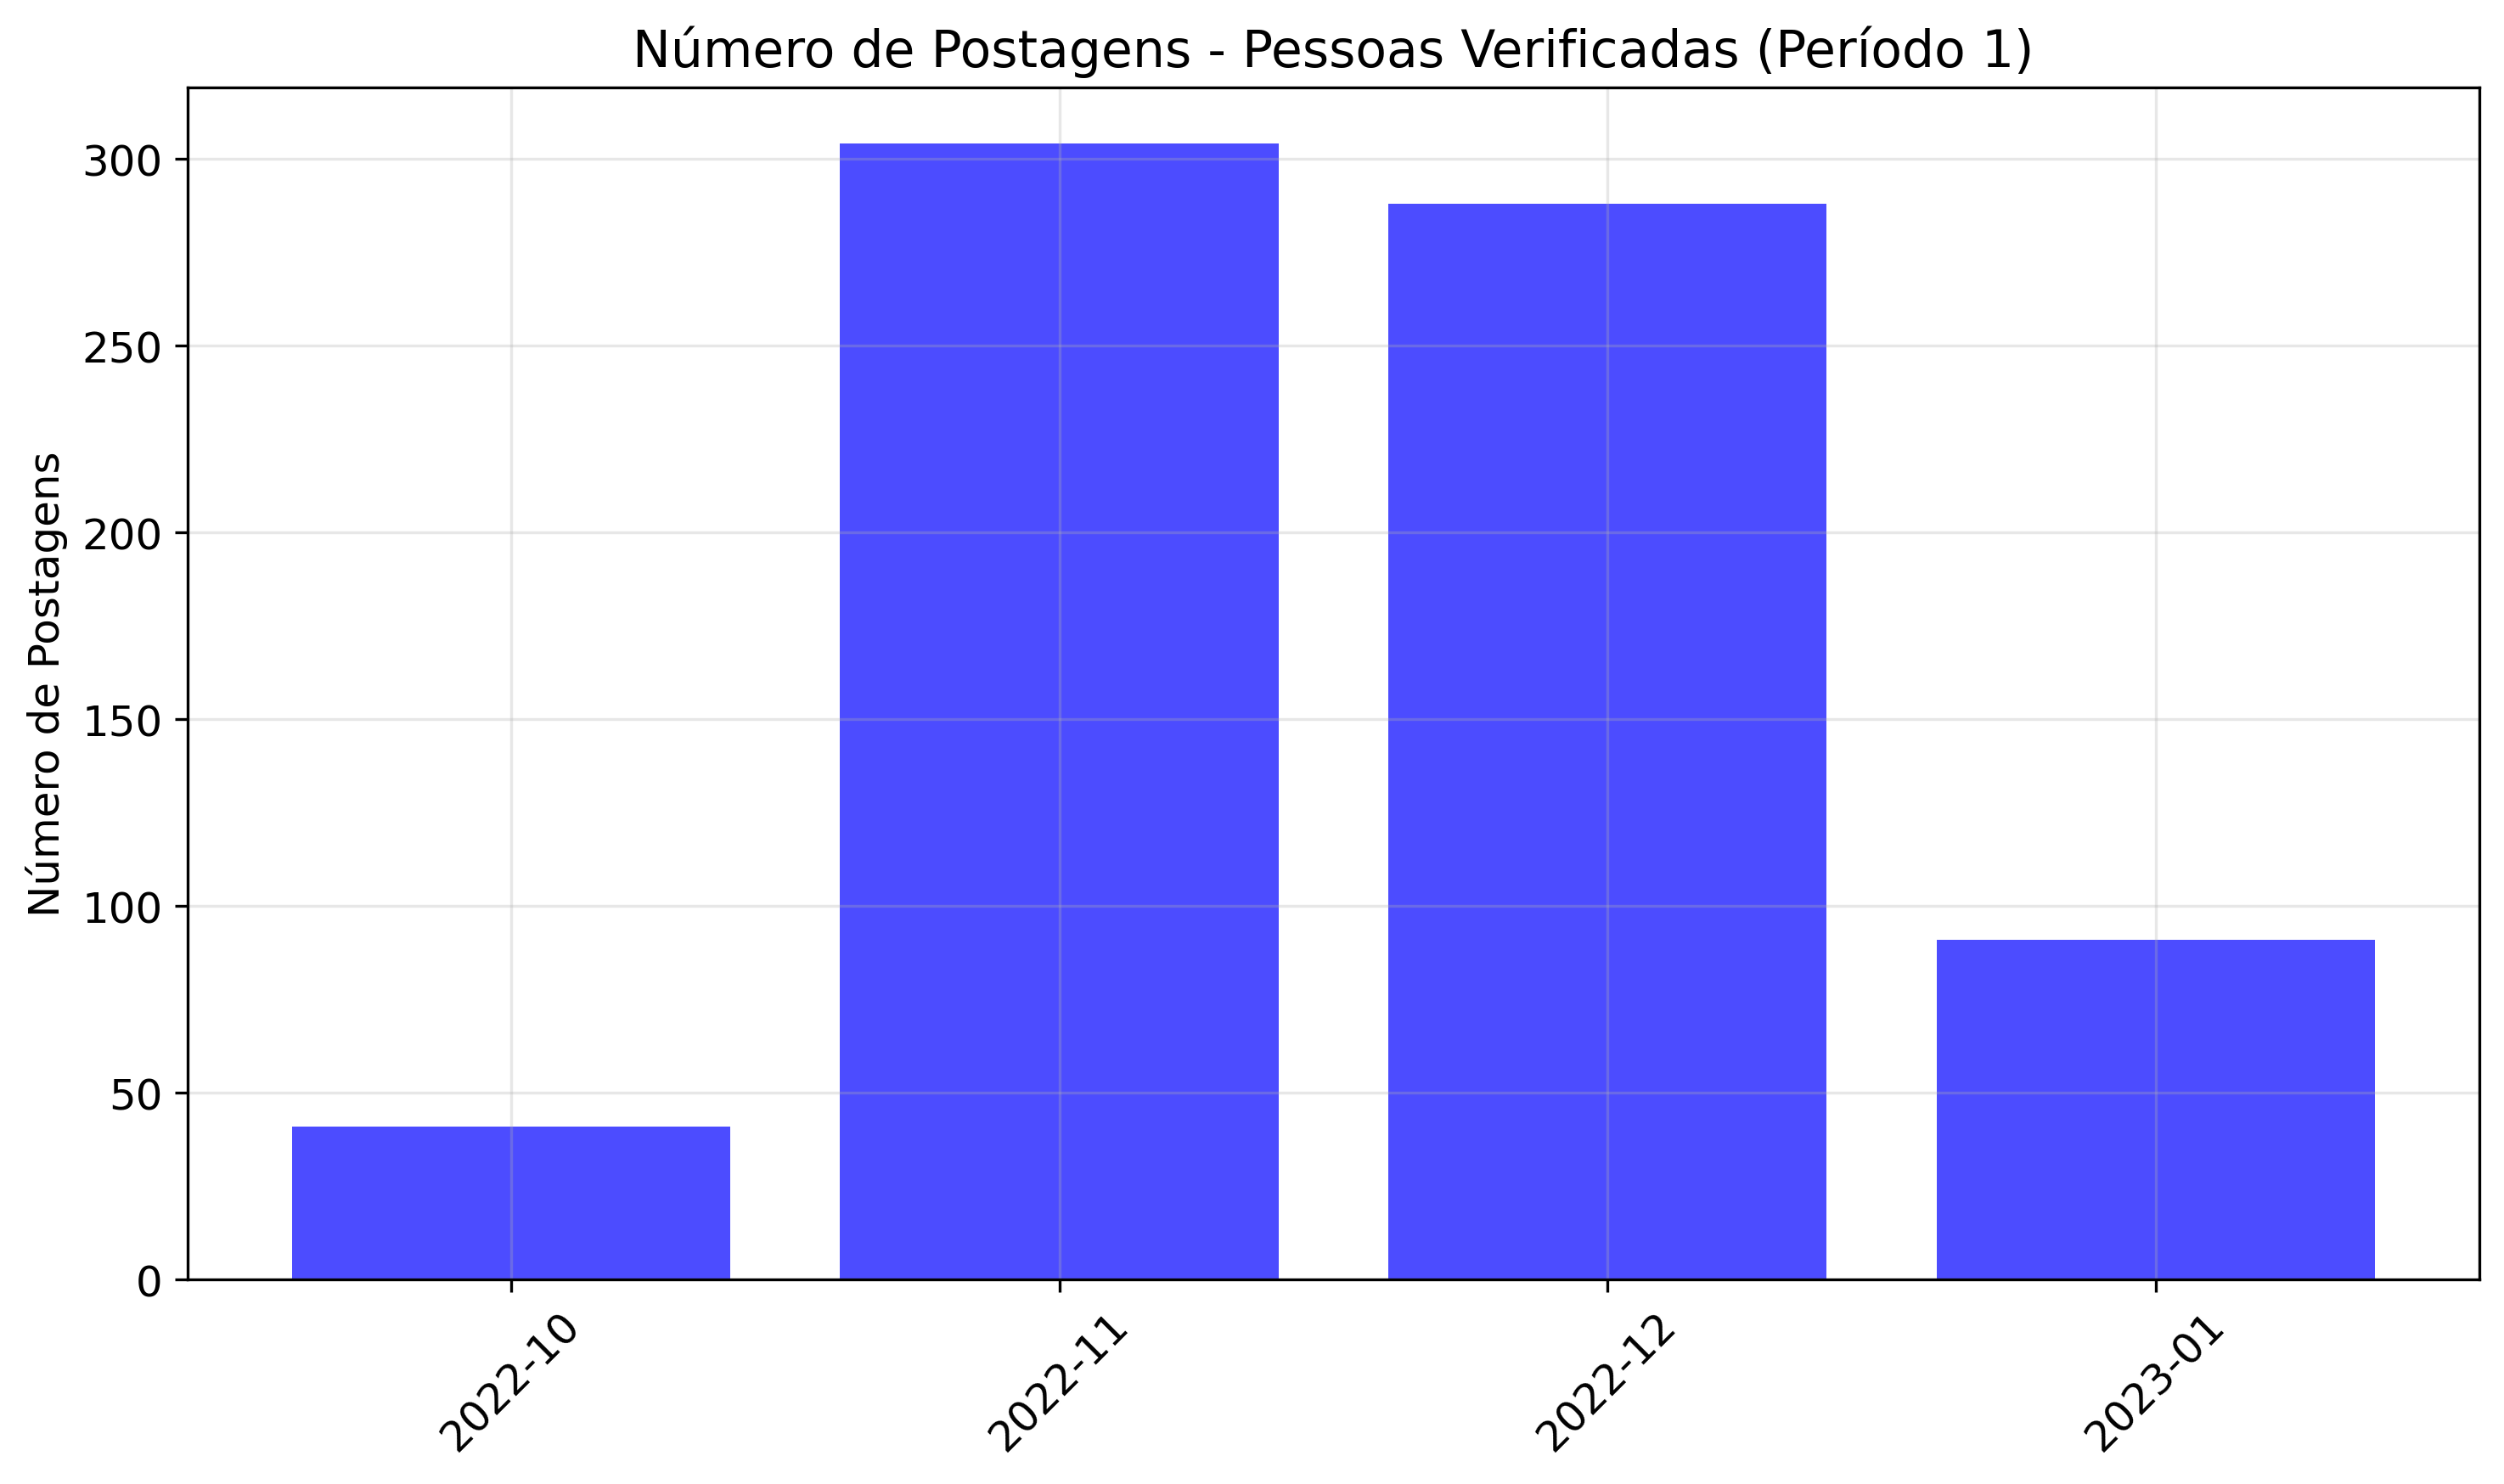
\includegraphics[width=0.8\textwidth]{figura25_postagens_verificadas_periodo1.png}
\caption{Número de postagens das pessoas verificadas no período 1 (30/10/2022 a 08/01/2023).}
\label{fig:figura25}
\end{figure}

\begin{figure}[h]
\centering
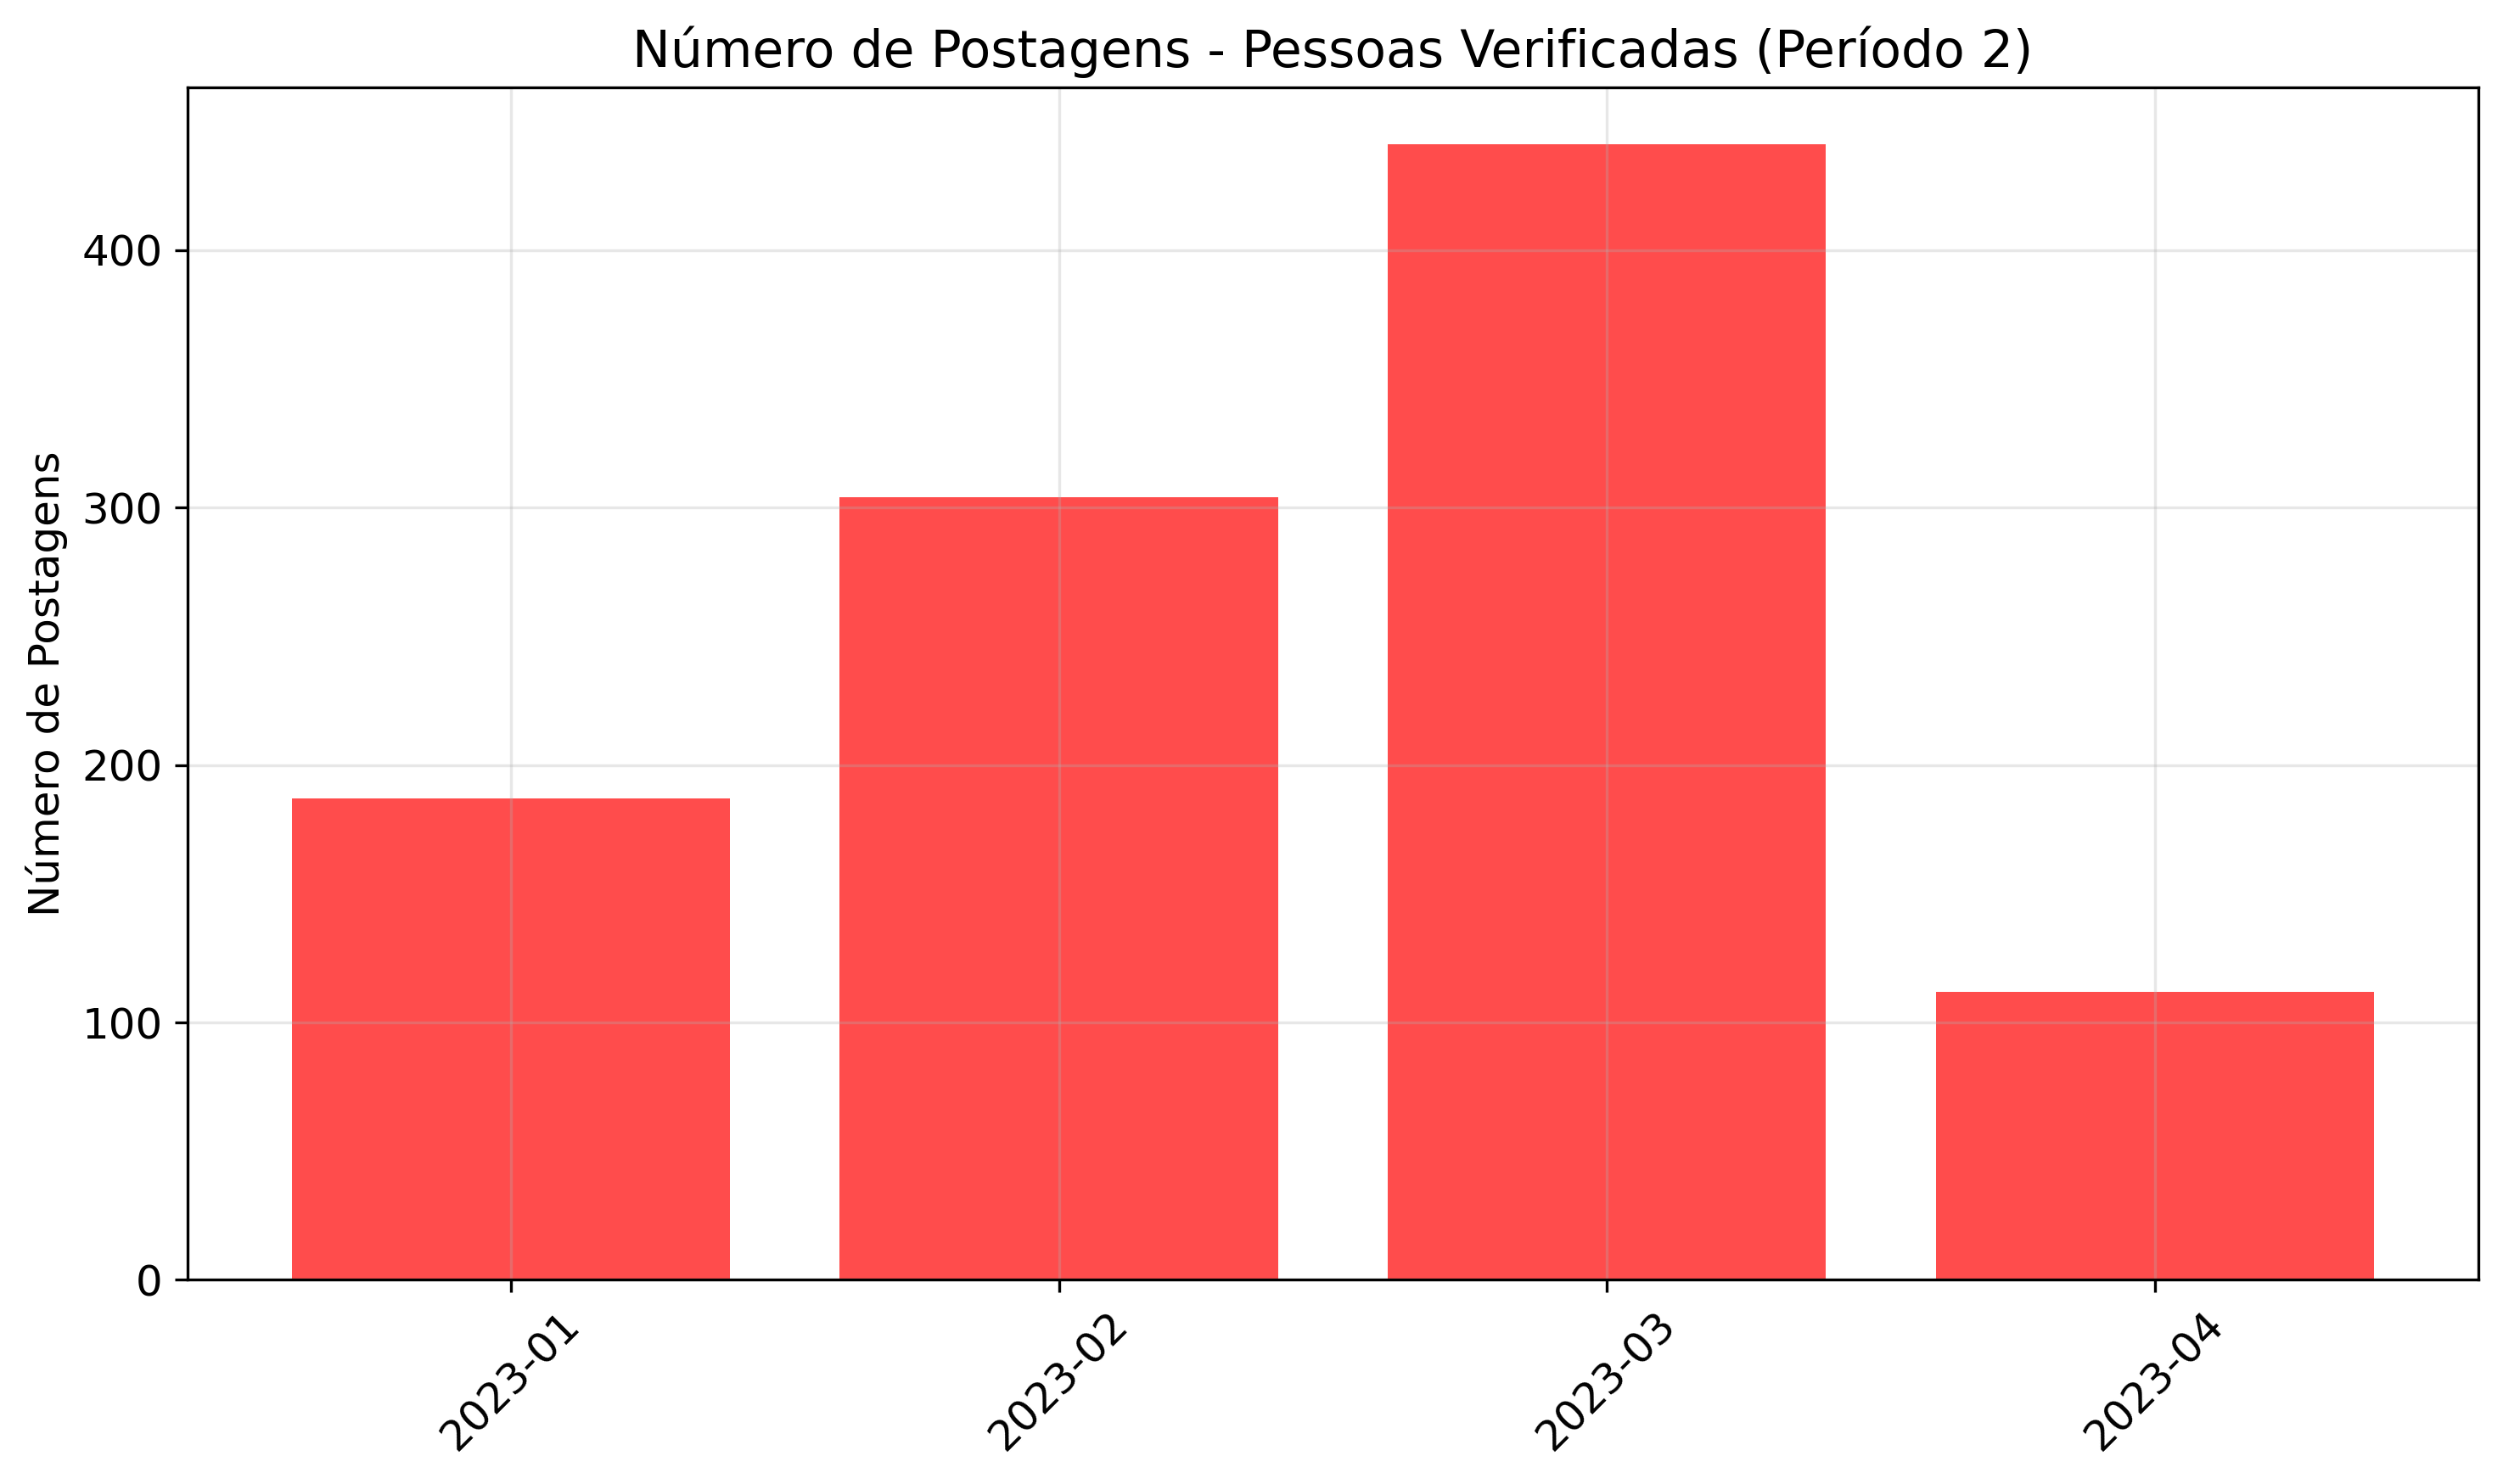
\includegraphics[width=0.8\textwidth]{figura26_postagens_verificadas_periodo2.png}
\caption{Número de postagens das pessoas verificadas no período 2 (09/01/2023 a 10/04/2023).}
\label{fig:figura26}
\end{figure}

\begin{figure}[h]
\centering
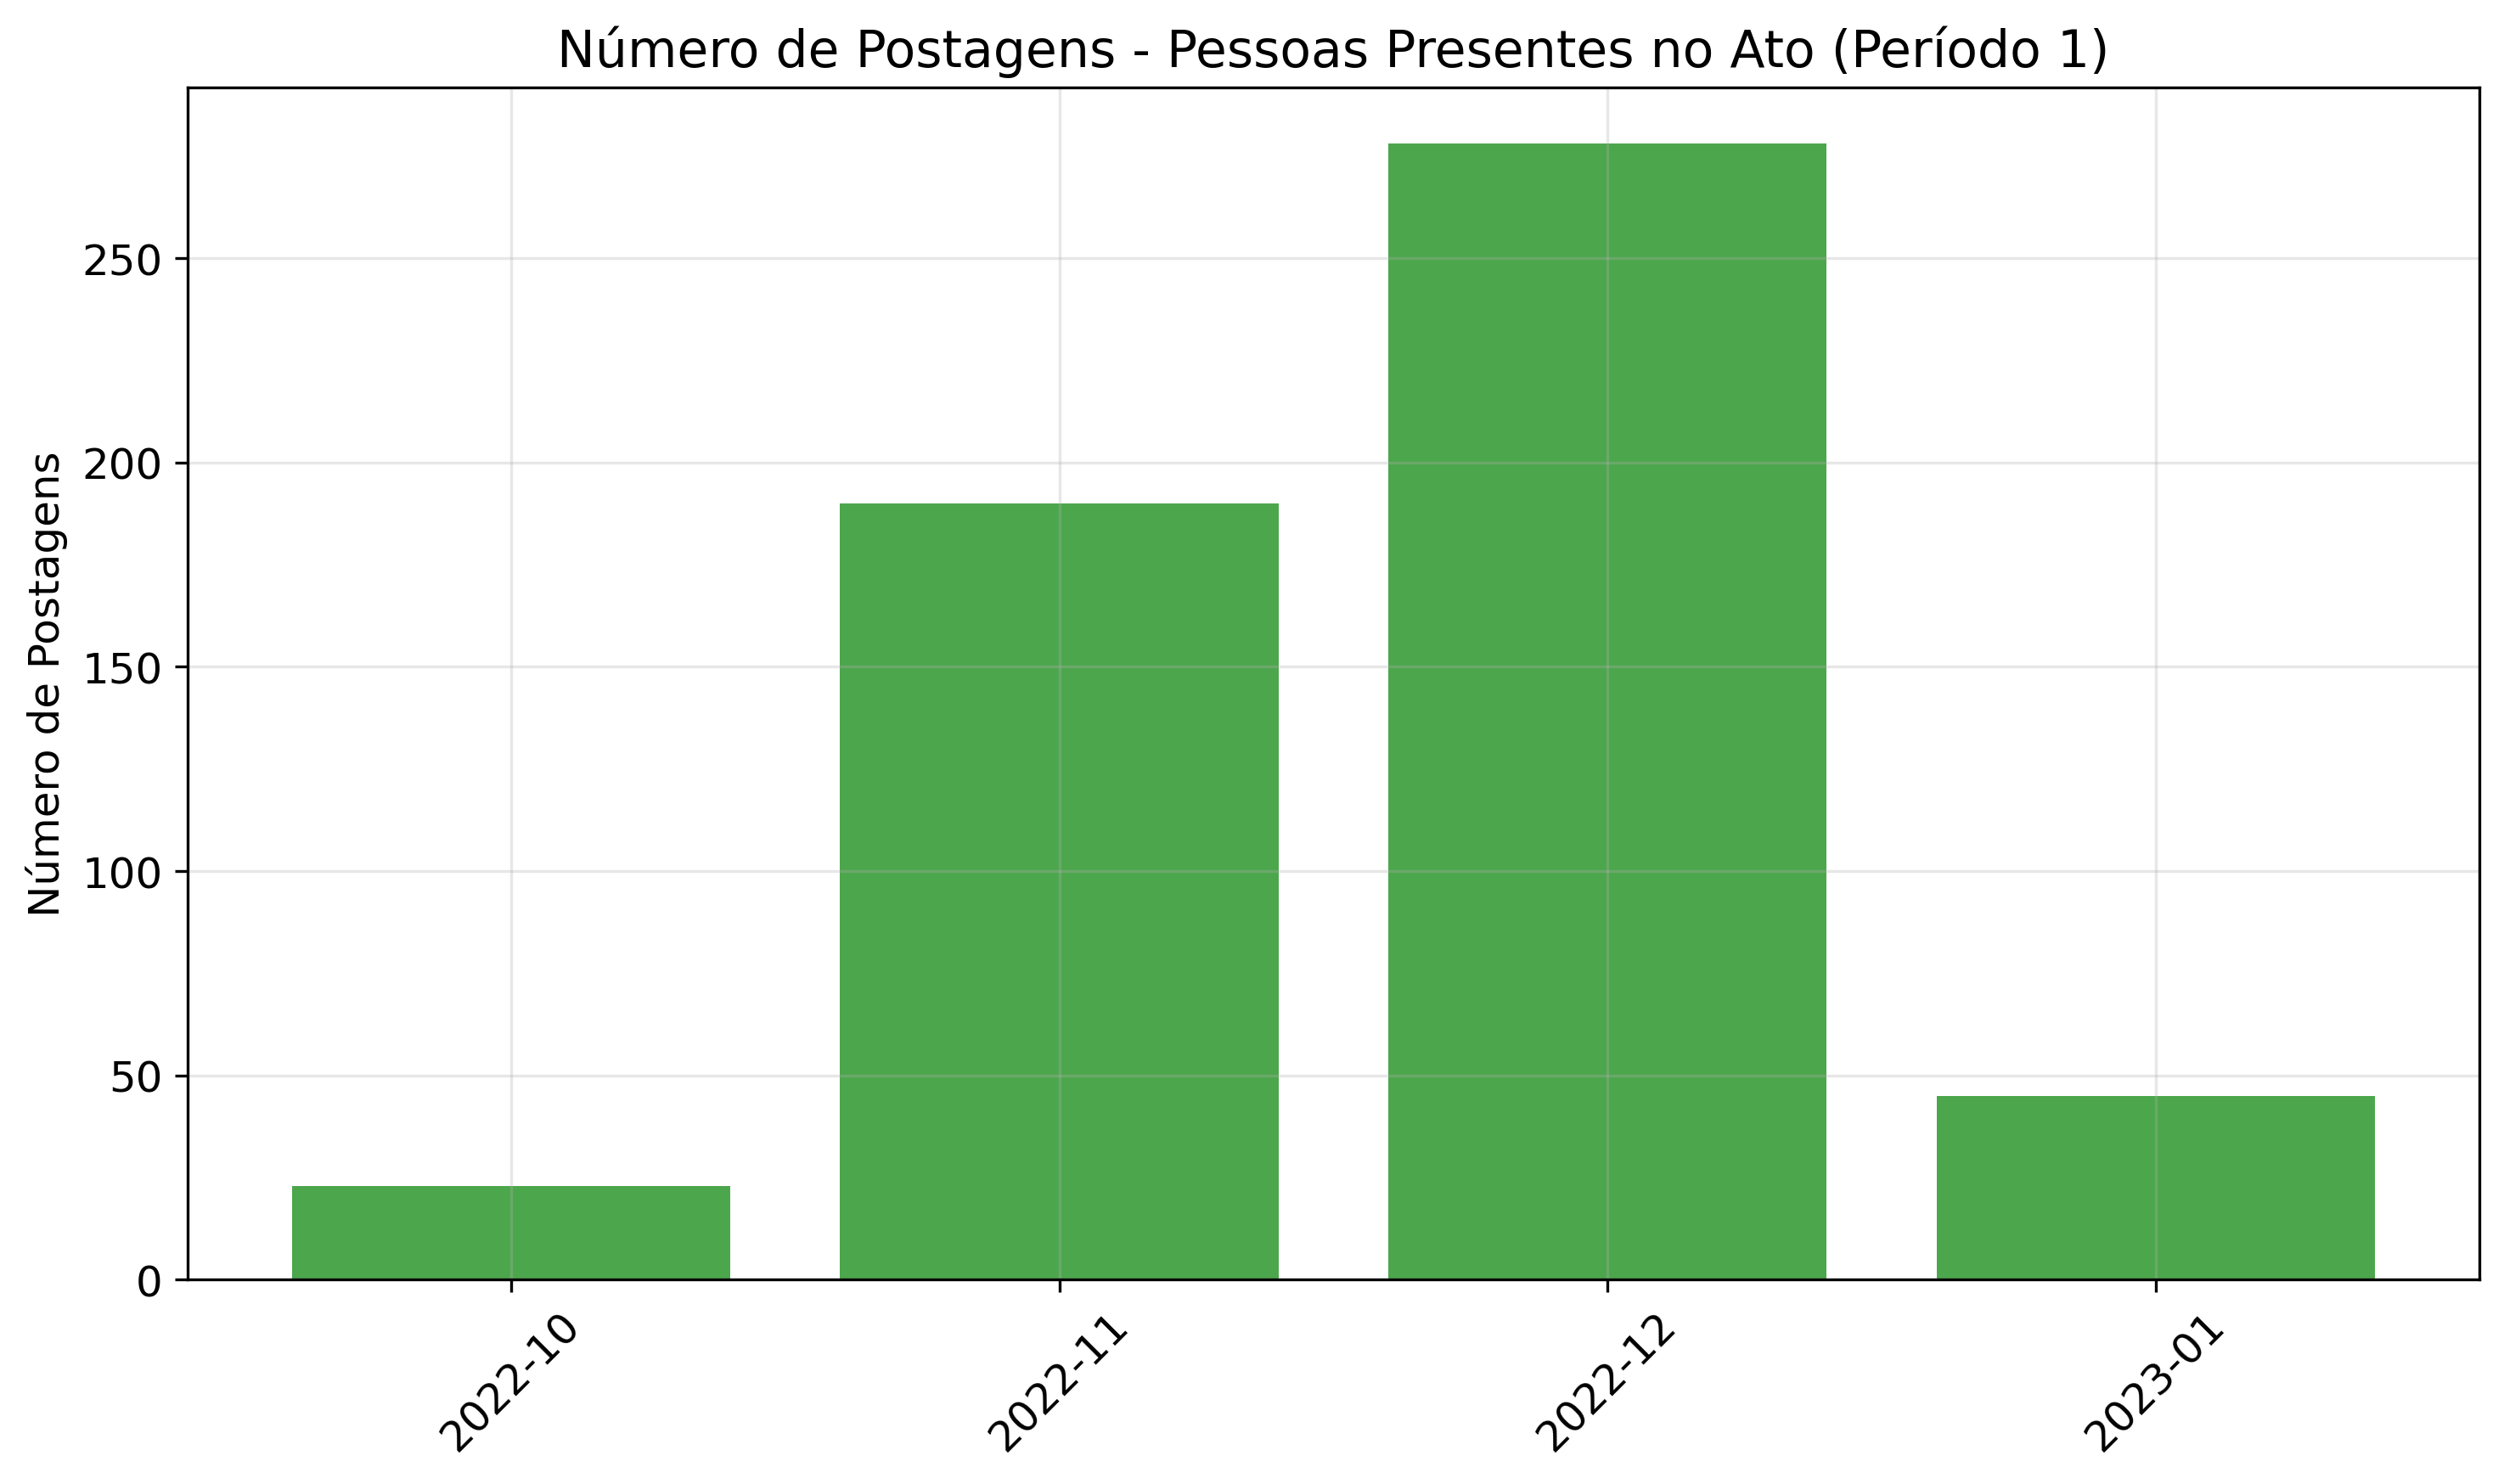
\includegraphics[width=0.8\textwidth]{figura27_postagens_presentes_periodo1.png}
\caption{Número de postagens das pessoas presentes no ato no período 1 (30/10/2022 a 08/01/2023).}
\label{fig:figura27}
\end{figure}

\begin{figure}[h]
\centering
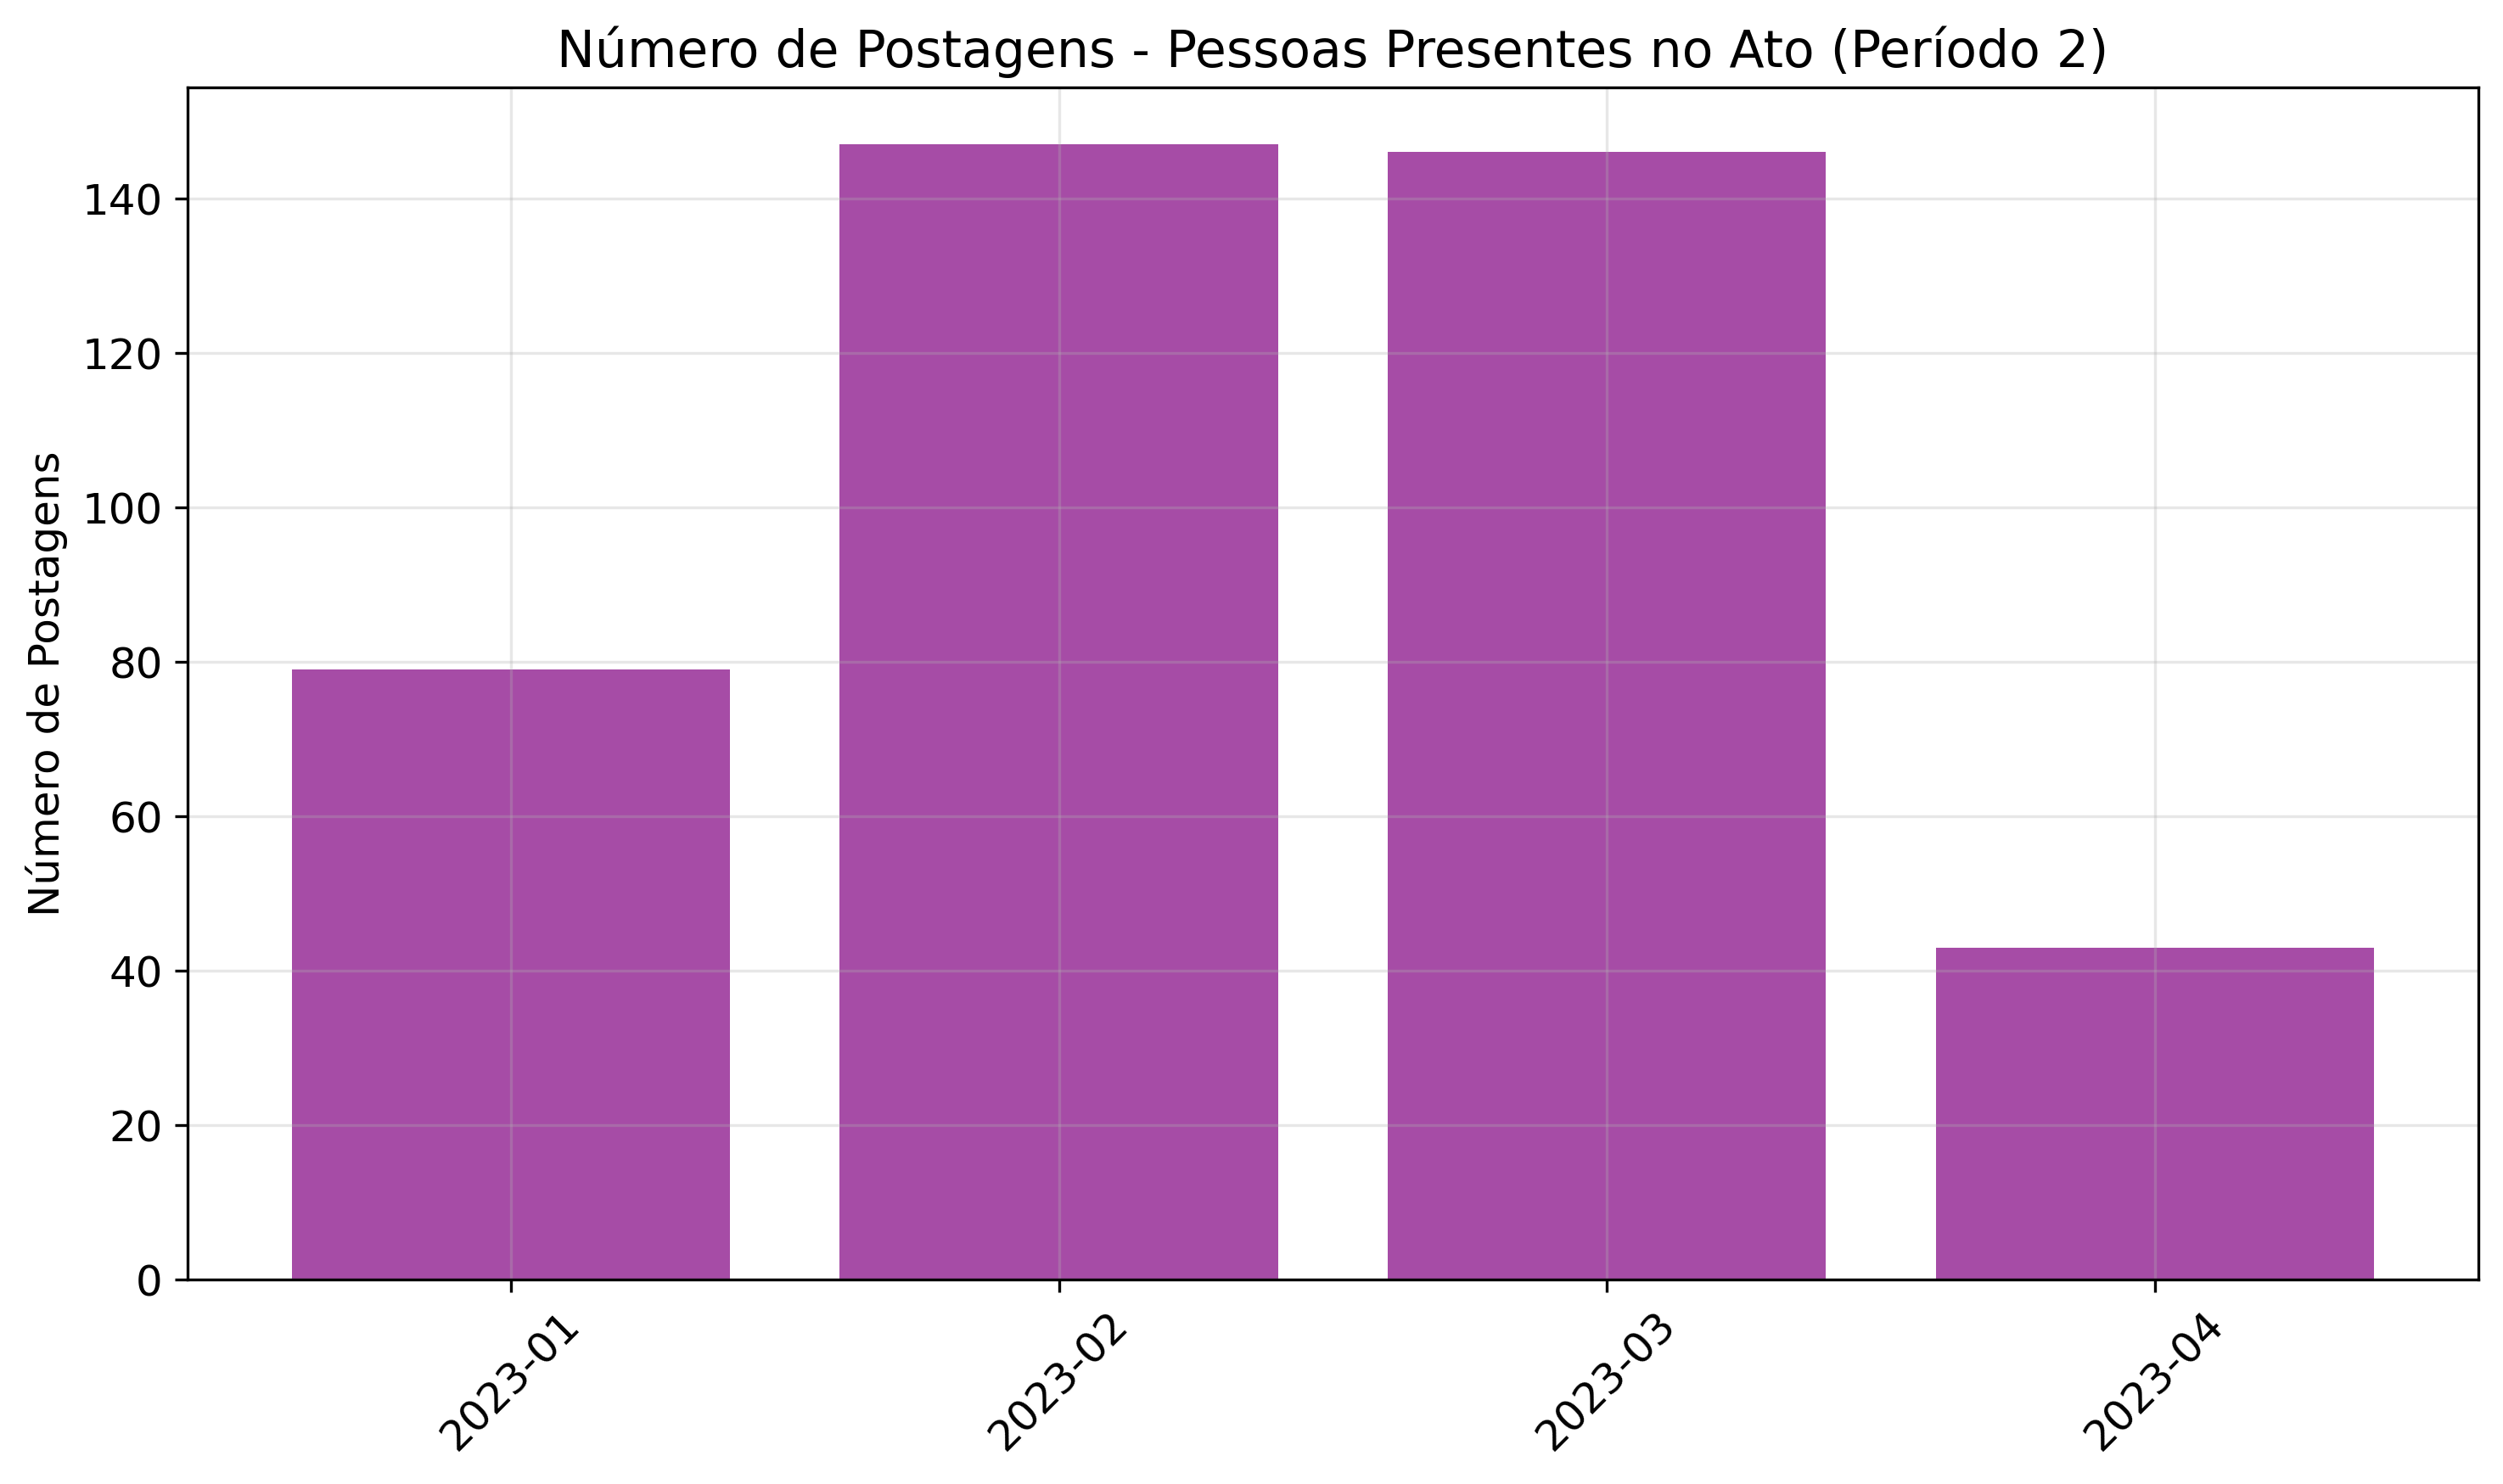
\includegraphics[width=0.8\textwidth]{figura28_postagens_presentes_periodo2.png}
\caption{Número de postagens das pessoas presentes no ato no período 2 (09/01/2023 a 10/04/2023).}
\label{fig:figura28}
\end{figure}

Comparando os diferentes períodos, observa-se que as pessoas verificadas mantiveram uma quantidade de postagens relativamente estável antes do ato, porém nos meses seguintes, após Janeiro, aumentaram significativamente a quantidade de postagens. No caso dos presentes no ato, observa-se que houve uma diminuição drástica de postagens no período imediatamente após o ato, comparado aos meses anteriores. A frequência voltou a valores normais, porém ainda levemente menores que os observados antes do ato.

\section{Avaliação e Discussão}

\subsection{Análise de sentimentos}

\subsubsection{Pessoas verificadas}

A análise diária, presente nas Figuras 1 e 2, é interessante quando o desejo é analisar os sentimentos em dias específicos. Olhando para os resultados obtidos, pode-se obter informações sobre os sentimentos dos autores nos picos do gráfico, representando acontecimentos do dia em questão. Como exemplo, é visto que no dia 18/12/2022, a Figura 1 teve seu pico mais positivo na análise das descrições das postagens, muito provavelmente por conta da final da Copa do Mundo, que ocorreu no mesmo dia. Já no dia 12/12/2022, houve a cerimônia de diplomação do presidente atualmente eleito\footnote{Fonte: https://g1.globo.com/politica/noticia/2022/12/12/lula-e-alckmin-participam-de-cerimonia-de-diplomacao-no-tribunal-superior-eleitoral.ghtml} e como visualizado no gráfico de descrições, esse é um dos dias com os sentimentos mais negativos. Agora, olhando para a Figura 2, é visto que há o pico de sentimentos positivos no texto das imagens no dia 15/01/2023, sendo que dois dias antes foi definido que o ex-presidente Jair Bolsonaro seria investigado pelos ataques do dia 08/01\footnote{Fonte: https://www.bbc.com/portuguese/brasil-64271602}. Esse sentimento positivo pode indicar postagens de apoio ao ex-presidente. Dois dias depois, há uma queda nesses sentimentos, muito provavelmente, pelo mesmo motivo. Em algumas imagens do período após o dia 8, também é observado um pico de sentimento positivo no dia 21/03/2023. Houve dois acontecimentos nesse dia que podem explicar isso: no dia anterior, a deputada do PSOL, Erika Hilton, pediu à Procuradoria-Geral da República (PGR) um pedido de suspensão dos perfis nas redes sociais do também deputado Nikolas Ferreira\footnote{Fonte: https://www.cnnbrasil.com.br/politica/moraes-manda-pgr-se-manifestar-sobre-pedido-de-suspensao-de-perfis-de-nikolas-ferreira/} e nesse mesmo dia, Michelle Bolsonaro lançou sua linha de produtos cosméticos\footnote{Fonte: https://www.estadao.com.br/politica/michelle-bolsonaro-lanca-linha-de-produtos-cosmeticos/}.

Olhando agora para as análises mensais, na Figura 5, é visto que os sentimentos começam com um valor médio menor, o que é explicado pelo período de análise começar logo após o fim das eleições, Apenas em novembro, tem-se uma média maior que 0.20, o que pode indicar que o ímpeto de mobilização e de chamado ocorreu nesse período de maneira intensa e posteriormente, foi visto que o valor médio desse sentimento caiu, o que indica a presença de sentimentos negativos presentes nas postagens desde então.

Já para essa mesma lista de pessoas, porém olhando agora para o período após o dia 8, na Figura 6, é visto que o sentimento médio caiu bastante de janeiro a fevereiro, o que indica as postagens negativas referentes ao ocorrido no ato.

\subsubsection{Presentes no ataque}

Para a lista de presentes no ataque, também é possível analisar alguns dias separadamente. Agora, olhando para a análise de sentimentos na descrição, da Figura 3, percebe-se que o dia 31/12/2022 foi o de maior sentimento positivo, o que faz sentido, visto que essa é uma data comemorativa, onde geralmente as pessoas desejam boas energias. Já quando o foco é o texto das imagens, ainda na Figura 3, há um pico de sentimento negativo no dia 22/11/2022, o que pode ser entendido como muitas mensagens de ódio ao atual presidente, visto que até o dia anterior, ele estava internado para uma retirada de lesão na laringe\footnote{Fonte: https://www.cnnbrasil.com.br/politica/lula-tem-alta-apos-internacao-para-retirada-de-lesao-na-laringe-no-domingo-20/\#:\~:text=Lula\%20recebeu\%20alta\%20nesta\%20segunda,foram\%20detectados\%20sinais\%20de\%20câncer.}. Na análise do texto das imagens na Figura 4, é possível ver um pico negativo no dia 08/04/2023, o que pode ser explicado por uma notícia do dia anterior, que diz que o Governo retirou os Correios e outras empresas estatais do programa de privatização\footnote{Fonte: https://g1.globo.com/politica/noticia/2023/04/07/governo-retira-correios-e-outras-estatais-de-programas-de-privatizacao.ghtml}.

Analisando os sentimentos mensais da Figura 7, em novembro houve uma queda nos sentimentos, provavelmente por conta do resultado das eleições e em janeiro também ocorreu esse fenômeno, o que pode ter sido por estar se aproximando do ato e os discursos estarem alinhados ao ataque. Além disso, na Figura 8, é observado que janeiro foi o pior mês possível quanto aos sentimentos.

Observando a Figura 10 e 11, é fácil perceber que houve uma diferença de discurso positivo para negativo antes e depois do ato, além da redução do número de postagens. Isso acontece porque muitos desses usuários foram detidos e seus perfis foram bloqueados, ou até mesmo apagados. Além disso, muitas postagens referentes ao ato e com mais discursos negativos foram apagadas, restando apenas as positivas.

\subsection{Análise de palavras}

\subsubsection{Pessoas verificadas}

A análise das nuvens de palavras de menções revelou uma interessante tendência após o dia 8, com uma nítida diminuição nas marcações relacionadas ao ex-presidente Jair Bolsonaro e à sua mulher, Michelle Bolsonaro. Essa redução nas menções a ambos os indivíduos sugere uma possível mudança na forma como são percebidos e discutidos. Esses resultados instigam reflexões sobre os fatores que podem estar influenciando essa diminuição e sobre o impacto que isso pode ter no cenário político atual. Já para as nuvens de palavras gerais, não houveram muitas alterações nesses períodos.

\subsubsection{Presentes no ataque}

Sobre a nuvem de menções, houve um aumento nas menções ao ex-presidente, provavelmente como apoio, mas em contrapartida, menções relacionadas ao exército, como 35bi\_exercito, marinhaoficial, exercito\_oficial e menções a grandes canais de comunicação, como cbstv, foxnews, nbcnews, entre outros, eram muito mais utilizados no período pré-ataque. Esse resultado é condizente com a realidade, visto que estavam sendo pedidos tentativas de intervenção militar, além dos protestos contra o resultado das eleições estarem ocorrendo constantemente.

Após o ocorrido, houve uma clara mudança nas descrições relacionadas ao ataque, com um foco maior em temas como Lula, Haddad e Bolsonaro. No entanto, ao analisarmos a nuvem de palavras anterior, observamos uma variedade de termos na descrição, o que indica uma dispersão de ideias. Visto que são pessoas que não estão envolvidas com política constantemente como os verificados, é comum que a nuvem de palavras aqui fique mais dispersa entre diversos assuntos diferentes.

\subsection{Número de postagens}

\subsubsection{Pessoas verificadas}

Analisando o número médio de postagens nas Figuras 25 e 26, é visto que ocorreu um aumento de postagens após o ato do dia 8 de janeiro, provavelmente postagens com o intuito de minimizar ou alterar discursos contra o ataque e demonstrando apoio ao atual presidente, por conta das investigações voltadas a ele.

\subsubsection{Presentes no ataque}

Já para o conjunto de dados de presentes no ataque, há um resultado esperado, o número de postagens diminuiu, principalmente no mês de janeiro. Isso ocorreu porque muitos desses perfis pararam de postar após o fatídico dia ou até mesmo perderam o acesso às suas contas. Analisando as contas do \textit{Instagram} desses usuários, é possível notar que a última postagem de muitos deles foi justamente no dia 8.

\section{Conclusão}

Este artigo teve como objetivo analisar a evolução do discurso no Instagram dos agentes envolvidos na tentativa de golpe ocorrida no dia 8 de janeiro de 2023 em Brasília, quando centenas de apoiadores do ex-presidente Jair Bolsonaro invadiram os prédios do Congresso Nacional, Palácio do Planalto e Supremo Tribunal Federal. Para isso, foram coletados e analisados os dados de postagens de dois grupos de agentes: pessoas verificadas associadas ao ex-presidente e pessoas presentes no ataque. A análise foi realizada por meio de ferramentas de análise de sentimentos e de nuvem de palavras, comparando os períodos antes e depois do ataque.

Os resultados mostraram que houve uma mudança significativa no discurso desses agentes, tanto em termos de frequência quanto de conteúdo, bem como na interação com o público. Os agentes verificados aumentaram o número e a radicalização das postagens nos meses anteriores ao ataque, buscando mobilizar e influenciar seus seguidores. Após o ataque, esses agentes diminuíram as menções ao ex-presidente e à sua mulher, sugerindo uma possível mudança na forma como são percebidos e discutidos. Os agentes presentes no ataque também aumentaram o número e a radicalização das postagens nos meses anteriores ao ataque, expressando ódio ao atual presidente e pedindo intervenção militar. Após o ataque, esses agentes diminuíram ou modificaram suas postagens, em resposta às consequências jurídicas e políticas de seu envolvimento.

Este estudo contribui para o conhecimento sobre o uso do Instagram em contextos políticos, especialmente em situações de conflito ou de crise. Ele revela como as plataformas digitais podem ser usadas para disseminar notícias falsas e teorias conspiratórias, mobilizar e influenciar seguidores, e incitar a violência e a desestabilização democrática. Ele também aponta para os desafios e as limitações da pesquisa nessa área, como a dificuldade de coletar dados de perfis bloqueados ou apagados, ou a possibilidade de viés na seleção dos agentes envolvidos na tentativa de golpe.

Como recomendações para futuras pesquisas, sugere-se ampliar o escopo da análise para incluir outras plataformas digitais, como WhatsApp, Telegram e Facebook, que também foram usadas pelos agentes da tentativa de golpe. Por fim, sugere-se realizar uma análise qualitativa das postagens, buscando compreender as motivações, as crenças e as identidades dos agentes envolvidos na tentativa de golpe.

\section{Agradecimentos}

Agradecemos a todos que colaboraram com este trabalho, em especial, ao Silas por ter nos ajudado tanto na obtenção de dados, quanto no que deveríamos estudar. Também agradecemos à prof.ª Jonice, por ter nos permitido estudar o tema e mostrar as ferramentas necessárias para a obtenção dos resultados.

\bibliographystyle{ACM-Reference-Format}
\bibliography{referencias}

\end{document} 